% TODO L04 FEATURE MODELING

\ifuniversity{recording}{\date{April 26, 2023}\setpicture[50]{ovgu-autumn3}\setcopyright{Photo: Hannah Theile (OVGU)}}
\ifuniversity{ulm}{\date{May 4, 2023}\setpicture[200]{may21-south}}
\ifuniversity{magdeburg}{\setpicture[50]{ovgu-autumn3}\setcopyright{Photo: Hannah Theile (OVGU)}}
\ifuniversity{bern}{\setpicture[50]{unibe_00517_200609_1200}}
\ifuniversity{paderborn}{\date{May 8, 2024}\setpicture[350]{image9}}
\ifuniversity{indonesia}{\date{February 17, 2025}}
\ifuniversity{braunschweig}{\date{November 6, 2024}}

\author{Elias Kuiter, Thomas Thüm, Timo Kehrer}
\lecture{Feature Modeling}{modeling}

\section{Feature Models and Configurations}
\subsection{Recap: Software Product Lines}
\begin{frame}{\myframetitle\ \mytitlesource{\lectureintroduction}}
	\begin{fancycolumns}[t]
		\begin{definition}{Software Product Line \mysource{\seiwhitepaperspl\mypage{5}}}
			\mycitebegin A \emph{software product line} is 
			\begin{itemize}
				\item a set of software-intensive systems
				\item that share a common, managed set of features
				\item satisfying the specific needs of a particular market segment or mission
				\item and that are developed from a common set of core assets in a prescribed way.\myciteend
				\mysource{\href{https://resources.sei.cmu.edu/library/asset-view.cfm?assetID=513819}{Software Engineering Institute, Carnegie Mellon University}}
			\end{itemize}
		\end{definition}
		\begin{definition}{Product \mysource{\fospl\mypage{19}}}
			\mycite{A \emph{product of a product line} is specified by a valid feature selection (a subset of the features of the product line). A feature selection is \emph{valid} if and only if it fulfills all feature dependencies.}
		\end{definition}
	\nextcolumn
		\begin{definition}{Feature \mysource{\fospl\mypage{18}}}
			\mycite{A \emph{feature} is a characteristic or end-user-visible behavior of a software system.}
		\end{definition}
		\centering\xkcd{2369}{width=.9\linewidth,trim=35 35 35 35,clip}
	\end{fancycolumns}
\end{frame}

\subsection{Features Have Dependencies}

\begin{frame}{\myframetitle}
	\begin{fancycolumns}[columns=3,widths={40,20,40}]
		\myexampletight{Ordering a Waffle \ldots}{
			\pic[width=\textwidth]{waffle-feature-model}
		}
		\nextcolumn
		\myexampletight{\ldots with Sugar}{
			\pic[width=\textwidth]{waffle-sugar}
		}
		\myexampletight{\ldots with Cherries}{
			\pic[width=\textwidth]{waffle-cherries}
		}
		\nextcolumn
		\begin{note}{This is Nice, But \ldots}
			\begin{itemize}
				\item plate and sugar seem to always be included, a fork is only included for some orders\\
					$\Rightarrow$ limitations seem \emph{arbitrary}
				\item children get special treatment\\
					$\Rightarrow$ order process is \emph{unfair}
				\item what exactly am I paying for?\\
					$\Rightarrow$ investments are \emph{unclear}
			\end{itemize}
		\end{note}
		\begin{definition}{In This Lecture}
			\begin{enumerate}
				\item how to \emph{model and configure} features and their dependencies?
				\item how to \emph{store and communicate}?
				\item how to \emph{analyze and understand}?
			\end{enumerate}
		\end{definition}
	\end{fancycolumns}
\end{frame}

\subsection{Specifying Valid Configurations}

\newcommand{\feat}[1]{{\emph{#1}}}
\newcommand{\exampleFeatureSetConfigDB}{
	\vspace*{-3ex}
	\begin{align*}
		\text{Feature set } F = \{&\textbf{C}onfigDB, \textbf{G}et, \textbf{P}ut, \textbf{D}elete,\\
		&\textbf{T}ransactions, \textbf{W}indows, \textbf{L}inux\}
	\end{align*}
}

\begin{frame}{\myframetitle}
	\begin{fancycolumns}
		\begin{definition}{Configuration}
			\begin{itemize}
				\item a \emph{configuration} \deutsch{Konfiguration} over a set of features $F$ selects and deselects features in $F$
				\item formally: a pair $(S, D)$ such that $S, D \subseteq F$ and $S, D$ are disjoint ($S \cap D = \varnothing$)
				\item is \emph{complete} \deutsch{vollständig} if all features are covered ($S \cup D = F$) and \emph{partial} \deutsch{partiell} otherwise
				\item a complete configuration is \emph{valid} \deutsch{gültig} if it ``makes sense'' in the domain and \emph{invalid} \deutsch{ungültig} otherwise % TODO why only complete configurations? probably easier to understand here, but validity could also be useful for partial configurations later
				\item we often abbreviate complete configurations with $S \equiv (S, F \setminus S)$
			\end{itemize}
		\end{definition}
	\nextcolumn
		\myexample{}{
			\exampleFeatureSetConfigDB
			Examples for \emph{complete} configurations:
			\begin{itemize}
				\item \emph{valid} (read-only database on Windows):
					$\cfg{C, G, W}{P, D, T, L}$
				\item \emph{valid} (fully functional database on Linux):
					$\cfg{C, G, P, D, T, L}{W}$
				\item \emph{invalid} ($\lightning$ no operating system):
					$\cfg{C, G}{P, D, T, W, L}$
				\item \emph{invalid} (transactions $\lightning$ read-only database):
					$\cfg{C, G, T, L}{P, D, W}$
			\end{itemize}
			Examples for \emph{partial} configurations:
			
			$\cfg{C, G}{P, D}$, $(\varnothing, \varnothing)$
		}
	\end{fancycolumns}
\end{frame}

\subsubsection{Natural Language}

\begin{frame}{\myframetitle}\label{frame:natlang}
	\begin{fancycolumns}
		\begin{note}{Valid Configuration}
			A complete configuration over $F$ is valid if it ``makes sense'' in the domain.
			\emph{\color{lecturered}{$\leadsto$ ``makes sense''?}}
		\end{note}

		\begin{definition}{Natural Language}
			\begin{itemize}
				\item informal description of relationships between features in $F$
				\item a complete configuration $S$ is \emph{valid} if it conforms to the description
				\item[+] succinct
				\item[--] sometimes ambiguous
				\item[--] not machine-readable
			\end{itemize}
		\end{definition}
	\nextcolumn
		\myexample{}{
			``A \feat{configurable database} has an API that allows for at least one of the request types \feat{Get}, \feat{Put}, or \feat{Delete}.
			Optionally, the database can support \feat{transactions}, provided that the API allows for Put or Delete requests.
			Also, the database targets a supported operating system, which is either \feat{Windows} or \feat{Linux}.''
		}
	\end{fancycolumns}
\end{frame}

\subsubsection{Configuration Map}

\begin{frame}{\myframetitle}\label{frame:cfgmap}
	\begin{fancycolumns}
		\begin{note}{Valid Configuration}
			A complete configuration over $F$ is valid if it ``makes sense'' in the domain.
			\emph{\color{lecturered}{$\leadsto$ ``makes sense''?}}
		\end{note}

		\begin{definition}{Configuration Map}
			\begin{itemize}
				\item a \emph{configuration map} over $F$ is a set of complete configurations $M \subseteq \power{F}$
				\item a complete configuration $S$ is \emph{valid} if it occurs in the configuration map ($S \in M$)
				\item also known as product map
				\item[+] precise
				\item[--] not human-readable
				\item[--] redundant, explodes in size ($0 \leq \abs{M} \leq 2^{\abs{F}}$)
			\end{itemize}
		\end{definition}
	\nextcolumn
		\myexample{}{
			\exampleFeatureSetConfigDB
			Configuration map:\\\small
			\begin{fancycolumns}[animation=none]
				{\color{black}$\{C,G,W\}$}\\
				$\{C,P,W\}$\\
				$\{C,G,P,W\}$\\
				$\{C,D,W\}$\\
				$\{C,G,D,W\}$\\
				$\{C,P,D,W\}$\\
				$\{C,G,P,D,W\}$\\
				$\{C,P,T,W\}$\\
				$\{C,G,P,T,W\}$\\
				$\{C,D,T,W\}$\\
				$\{C,G,D,T,W\}$\\
				$\{C,P,D,T,W\}$\\
				$\{C,G,P,D,T,W\}$
			\nextcolumn
				$\{C,G,L\}$\\
				$\{C,P,L\}$\\
				$\{C,G,P,L\}$\\
				$\{C,D,L\}$\\
				$\{C,G,D,L\}$\\
				$\{C,P,D,L\}$\\
				$\{C,G,P,D,L\}$\\
				$\{C,P,T,L\}$\\
				$\{C,G,P,T,L\}$\\
				$\{C,D,T,L\}$\\
				$\{C,G,D,T,L\}$\\
				$\{C,P,D,T,L\}$\\
				{\color{black}$\{C,G,P,D,T,L\}$}
			\end{fancycolumns}
		}
	\end{fancycolumns}
\end{frame}

\subsubsection*{Configuration Map in Excel}

\begin{frame}{\myframetitle}
	\centering
	\picDark[width=0.48\linewidth]{products-in-excel}

	\textbf{Can we do better?}
\end{frame}

\subsection{Feature Models}

\subsubsection*{Syntax}

\begin{frame}{\myframetitle\ \mytitlesource{\fospl; \foda\mypages{63--72}; \batorygrammars}}
	\begin{fancycolumns}
		\centering
		\featureDiagramConfigurableDatabase
		
		\featureDiagramLegend
	\nextcolumn
		\begin{definition}{Feature Model \deutsch{Feature-Modell}}
			\begin{itemize}
				\item hierarchy of features
				\item dependencies between features modeled by tree and cross-tree constraints
				\item \emph{tree constraints}: defined by the hierarchy
				\item \emph{cross-tree constraints}: propositional formulas over features
				\item \emph{abstract features} are used to group other features
				\item \emph{concrete features} have an implementation
				\item also known as feature diagram or feature tree
				\item notation for \emph{optional/mandatory features} and \emph{or/alternative groups}
			\end{itemize}
		\end{definition}
	\end{fancycolumns}
\end{frame}

\subsubsection*{Semantics}

\begin{frame}{\myframetitle\ \mytitlesource{\fospl; \batorygrammars}}
	\begin{fancycolumns}[animation=none]
		\uncover<2-|handout:1>{
			\begin{definition}{Tree Constraints}
				\begin{itemize}
					\item the \emph{root feature} is always required
					\item each feature requires its parent (aka.~\emph{parent-child-relationship})
					\item an \emph{optional feature} can be (de-)selected freely when its parent is selected
					\item a \emph{mandatory feature} is required by its parent
					\item \emph{or group}: at least one child feature must be selected when the parent is selected
					\item \emph{alternative group}: exactly one child feature must be selected when the parent is selected
				\end{itemize}
			\end{definition}
		}
	\nextcolumn
		\centering
		\featureDiagramConfigurableDatabase
		\uncover<3|handout:1>{
			\begin{definition}{Cross-Tree Constraints}
				\begin{itemize}
					\item a list of \emph{propositional formulas} expressing further dependencies between features
					\item each cross-tree constraint must be satisfied
				\end{itemize}
			\end{definition}
		}
	\end{fancycolumns}
\end{frame}

\subsubsection*{Examples}

\begin{frame}{\myframetitle}
	\begin{fancycolumns}[animation=none]
		\centering
		\featureDiagramConfigurableDatabase[_fm]
		\featureDiagramOverlay{
			\only<2|handout:0>{
				\featureSelected{(ConfigDB_fm),(API_fm),(Get_fm),(OS_fm),(Windows_fm)}
				\featureDeselected{(Put_fm)(Delete_fm),(Transactions_fm),(Linux_fm)}
			}
			\only<3|handout:0>{
				\featureSelected{(ConfigDB_fm),(API_fm)(Transactions_fm)(OS_fm),(Get_fm)(Put_fm)(Delete_fm),(Linux_fm)}
				\featureDeselected{(Windows_fm)}
			}
			\only<4|handout:0>{
				\featureSelected{(ConfigDB_fm),(API_fm),(Get_fm)}
				\featureDeselected{(Put_fm)(Delete_fm)(Windows_fm)(Linux_fm),(Transactions_fm)(OS_fm)}
			}
			\only<5|handout:0>{
				\featureSelected{(ConfigDB_fm),(API_fm)(Transactions_fm)(OS_fm),(Get_fm),(Linux_fm)}
				\featureDeselected{(Put_fm)(Delete_fm)(Windows_fm)}
			}
		}
	\nextcolumn
		\myexample{Is This a Valid Configuration?}{
			\begin{itemize}
				\item<2-|handout:1> \emph{valid} (read-only database on Windows):
					$\cfg[2|handout:0]{C, A, G, O, W}{P, D, T, L}$
				\item<3-|handout:1> \emph{valid} (fully functional database on Linux):
					$\cfg[3|handout:0]{C, A, G, P, D, T, O, L}{W}$
				\item<4-|handout:1> \emph{invalid} ($\lightning$ no operating system):
					$\cfg[4|handout:0]{C, A, G}{P, D, T, O, W, L}$
				\item<5-|handout:1> \emph{invalid} (transactions $\lightning$ read-only database):
					$\cfg[5|handout:0]{C, A, G, T, O, L}{P, D, W}$
			\end{itemize}
		}
	\end{fancycolumns}
\end{frame}

\begin{frame}{\myframetitle}
	\begin{fancycolumns}[columns=3,widths={5,90,5},animation=none]
	\nextcolumn
		\centering
		\featureDiagramWaffle
		\begin{note}{}
			\begin{itemize}
				\item every feature (leaf or compound) can be abstract or concrete
				\item groups can be used anywhere
				\item directly below groups, no optional or mandatory markers are allowed
			\end{itemize}
		\end{note}
	\nextcolumn
	\end{fancycolumns}
\end{frame}

\subsection[Discussion]{Discussion of Feature Models}
\begin{frame}{\myframetitle}
	\begin{fancycolumns}[t]
		\begin{note}{Pro: Making Tacit Knowledge Explicit}
			\small\mycite{I think the best [about feature modeling] is you can see relationships, to actually know what configurations are allowed and what are not allowed. That was also not so easy to express in the past [\ldots] This is from the developer's point of view. But it's also [\ldots] important, because before we noticed that \emph{the same functionality was implemented twice} within the same project, basically they haven't realized that. They implemented the same features.} -- {\footnotesize Interview with Practitioners}\mysource{\href{https://link.springer.com/chapter/10.1007/978-3-319-11653-2_19}{Berger~et~al.~2014}}
		\end{note}

		\begin{note}{Pro: Tool Support} % TODO would be great to show more tool logos here from our community, and possibly also for commercial tools (upon request)
			\pic[width=.3\linewidth]{featureide-logo},\hspace{2mm}\href{https://biglever.com/solution/gears/}{Gears},\hspace{2mm}\href{https://www.pure-systems.com/de/purevariants}{pure::variants},\hspace{2mm}\ldots% end goal: the lecture shows how to realize a automated configurator that does not allow invalid configurations
		\end{note}
	\nextcolumn
		\begin{note}{Con: Challenges}
			\begin{itemize}
				\item \emph{domain scoping}: which features?
				\item \emph{feature interactions}: which dependencies?
				\item requires infrastructure, consulting, and training
			\end{itemize}
		\end{note}

		\vspace*{2mm}\centering\picDark[width=.85\linewidth]{wollmilchsau}
	\end{fancycolumns}
\end{frame}
 % this part is required to compile Part b
\lessonslearned{
	\item features, dependencies between features, and configurations
	\item feature models: abstract and concrete features, tree and cross-tree constraints
	\item tree constraints: optional, mandatory, or group, alternative group
}{ % TODO unify literature pointer (see Lecture 1-3)
	\item \fospl\mysection{2.3}\mypages{26--39}\\--- introduction to feature modeling
	\item Thorsten Berger et al. (2013): \href{https://doi.org/10.1145/2430502.2430513}{A Survey of Variability Modeling in Industrial Practice} % TODO is this really a good fit?

	\item Damir Nešić et al. (2019): \href{https://doi.org/10.1145/3338906.3338974}{Principles of Feature Modeling}
	% TODO refer to Kang et al. for introducing feature models? more references to other SPL books?
}{
	\begin{enumerate}
		\item sketch a feature model with features $A, B, C, D, E, F$ that has exactly those 5 valid configurations (pen and paper preferred):\\~

			\begin{fancycolumns}[t,columns=3,animation=none]
				$\{A,B\}$\\
				$\{A,B,D\}$\\~
			\nextcolumn
				$\{A,C,E\}$\\
				$\{A,C,F\}$\\
			\nextcolumn
				$\{A,C,E,F\}$\\
			\end{fancycolumns}

		\item discuss in groups whether your feature models are syntactically correct and specify exactly the above configurations
	\end{enumerate}

	\uploadpractice
}

\section{Transforming Feature Models}
\subsection{Representations and Transformations}

\begin{frame}[label=FeatureModelRepresentations]{\myframetitle}
	\begin{fancycolumns}[b]
		\begin{example}{Natural Language}
			\tiny ``A \feat{configurable database} has an API that allows for at least one of the request types \feat{Get}, \feat{Put}, or \feat{Delete}.
			Optionally, the database can support \feat{transactions}, provided that the API allows for Put or Delete requests.
			Also, the database targets a supported operating system, which is either \feat{Windows} or \feat{Linux}.''
		\end{example}
		\begin{example}{Configuration Map}
			\tiny
			\begin{fancycolumns}[animation=none]
				$\{C,G,W\}$\\
				\hspace{4mm}\vdots\\[1ex]
				$\{C,G,P,D,T,W\}$
			\nextcolumn
				$\{C,G,L\}$\\
				\hspace{4mm}\vdots\\[1ex]
				$\{C,G,P,D,T,L\}$
			\end{fancycolumns}
		\end{example}
		\begin{exampletight}{Feature Diagram (Graphical Feature Model)}
			\centering\tiny
			\featureDiagramConfigurableDatabase
		\end{exampletight}
	\nextcolumn
		\centering
		\sffamily
		\begin{tikzpicture}
			\tikzstyle{every edge}=[font=\tiny,draw,color=blue]
			\node (fd) at (2,0) [align=center] {Feature Model\\[-1ex]{\uncover<3->{\tiny\color{lecturered}Feature Diagram, \textbf{P1}}}};
			\node (nat) at (0,-2) [align=center] {Natural Language\\[-1ex]{\tiny\color{lecturered}Thoughts, Plain Text}};
			\node (cfg) at (4,-2) [align=center] {Configuration Map\\[-1ex]{\tiny\color{lecturered}Excel, Set of Sets}};

			\path [->] (fd) edge[bend left] node[sloped,yshift=1mm] {toString} (nat);
			\uncover<5->{\path [dotted, ->] (nat) edge[bend left] node[sloped,yshift=1mm] {\textbf{P3}} (fd);}
			
			\uncover<4->{\path [->] (fd) edge[bend left] node[sloped,yshift=1mm] {\textbf{P2}} (cfg);}
			\uncover<5->{\path [dotted, ->] (cfg) edge[bend left] node[sloped,yshift=1mm] {\textbf{P3}} (fd);}

			\node (trans) at (-1,-2.8) {};
			\node (trans2) at (2,-2.8) {};
			\node (trans3) at (-1,-3.1) {};
			\node (trans4) at (2,-3.1) {};
			\path [->] (trans) edge node[yshift=1mm] {Automated Transformation} (trans2);
			\path [dotted, ->] (trans3) edge[yshift=5mm] node[yshift=1mm] {Semi-Automated Transformation} (trans4);
		
			\node (bottomleft2) at (-0.2,-3.3) {\tiny\color{lecturered}Concrete Format};
		\end{tikzpicture}

		\begin{note}{Problems}
			\begin{enumerate}
				\item<3->[P1] How to express feature models \emph{textually}?
				\item<4->[P2] How to (a) validate configurations and (b) get all valid configurations \emph{automatically}?
				\item<5->[P3] \color{gray}{(How to reverse engineer feature models?)}
			\end{enumerate}
		\end{note}
	\end{fancycolumns}
\end{frame}

\subsection{UVL, the Universal Variability Language}

\begin{frame}[fragile]{\myframetitle\ \mytitlesource{\uvlwebsite}}
	\begin{fancycolumns}
\begin{uvltight}[basicstyle=\normalsize]{}
features
	ConfigDB
		mandatory
			API {abstract}
				or
					Get
					Put
					Delete

		optional
			Transactions
		mandatory
			OS {abstract}
				alternative
					Windows
					Linux

constraints
	Transactions => Put | Delete
\end{uvltight}
	\nextcolumn
		\begin{exampletight}{A Feature Model ``Sideways''}
			\centering
			\pic[width=\linewidth]{varied-model}
			$Transactions \pimplies Put \por Delete$
		\end{exampletight}
		\begin{note}{Universal Variability Language (UVL)}
			\begin{itemize}
				\item textual language for feature modeling
				\item adds advanced modeling constructs (e.g.,~attributes, cardinalities, submodels, \ldots)
			\end{itemize}
		\end{note}
	\end{fancycolumns}
\end{frame}

\begin{frame}{Representations and Transformations}
	\begin{fancycolumns}
		\centering
		\sffamily
		\begin{tikzpicture}
			\tikzstyle{every edge}=[font=\tiny,draw,color=blue]
			\node (fd) at (2,0) [align=center] {Feature Model\\[-1ex]{\tiny\color{lecturered}Feature Diagram, UVL}};
			\node (nat) at (0,-2) [align=center] {Natural Language\\[-1ex]{\tiny\color{lecturered}Thoughts, Plain Text}};
			\node (cfg) at (4,-2) [align=center] {Configuration Map\\[-1ex]{\tiny\color{lecturered}Excel, Set of Sets}};

			\path [->] (fd) edge[bend left] node[sloped,yshift=1mm] {toString} (nat);
			\path [dotted, ->] (nat) edge[bend left] node[sloped,yshift=1mm] {\textbf{P3}} (fd);
			
			\path [->] (fd) edge[bend left] node[sloped,yshift=1mm] {\textbf{P2}} (cfg);
			\path [dotted, ->] (cfg) edge[bend left] node[sloped,yshift=1mm] {\textbf{P3}} (fd);

			\node (trans) at (-1,-2.8) {};
			\node (trans2) at (2,-2.8) {};
			\node (trans3) at (-1,-3.1) {};
			\node (trans4) at (2,-3.1) {};
			\path [->] (trans) edge node[yshift=1mm] {Automated Transformation} (trans2);
			\path [dotted, ->] (trans3) edge[yshift=5mm] node[yshift=1mm] {Semi-Automated Transformation} (trans4);
		
			\node (bottomleft2) at (-0.2,-3.3) {\tiny\color{lecturered}Concrete Format};
		\end{tikzpicture}
	\nextcolumn
		\begin{note}{Problems}
			\begin{enumerate}
				\item[P1] How to express feature models \emph{textually}?
				\item[P2] How to (a) validate configurations and (b) get all valid configurations \emph{automatically}?
				\item[P3] \color{gray}{(How to reverse engineer feature models?)}
			\end{enumerate}
		\end{note}
		\begin{note}{Solutions}
			\begin{enumerate}
				\item[P1] Universal Variability Language $\Rightarrow$ \emph{Syntax}
				\item[P2] \emph{Semantics}?
				\item[P3] \color{gray}{--}
			\end{enumerate}
		\end{note}
	\end{fancycolumns}
\end{frame}
% TODO first show the simpler version of the tikz picture, then animate towards the above, animate together with text
% TODO do we really need this slide? semantics was already defined in Part 4a for feature models

\subsection{Propositional Formulas}

\subsubsection*{Recap}

\begin{frame}{\myframetitle}
	\begin{fancycolumns}
		\begin{definition}{Syntax of Propositional Formulas}
			Inductive definition of \emph{propositional formulas} \deutsch{aussagenlogische Formeln}
			\begin{itemize}
				\item the \emph{Boolean truth values} $\top$, $\bot$
				\item any \emph{Boolean variable} $X$
    			\item any \emph{negation} $\pnot \phi$ of a formula $\phi$
    			\item any \emph{conjunction} $(\phi \pand \psi)$ of formulas $\phi$ and $\psi$
				\item any \emph{disjunction} $(\phi \por \psi)$, \emph{implication} $(\phi \pimplies \psi)$, or \emph{biimplication} $(\phi \pequals \psi)$
			\end{itemize}
		\end{definition}
	\nextcolumn
		\begin{definition}{Informal Semantics of Propositional Formulas}
			\vspace*{-3ex}
			\begin{equation*}
				\begin{rcases}
					\top                \\
					\bot                \\
					\pnot \phi          \\
					\phi \pand \psi     \\
					\phi \por \psi      \\
					\phi \pimplies \psi \\
					\phi \pequals \psi
				\end{rcases} \text{ means } \begin{cases}
					\text{``true'' (or \emph{tautology})} \\
					\text{``false'' (or \emph{contradiction})} \\
					\text{``not $\phi$''} \\
					\text{``$\phi$ and $\psi$''} \\
					\text{``$\phi$ or $\psi$'' (inclusive or!)} \\
					\text{``if $\phi$, then $\psi$'' (and else?)} \\
					\text{``$\phi$ if and only if $\psi$''}
				\end{cases}
			\end{equation*}
		\end{definition}
		\begin{example}{Operator Precedence: $\pnot$, $\pand$, $\por$, $\pimplies$, $\pequals$}
			\vspace*{-3ex} % TODO Benno: why is this hack needed?
			\begin{align*}
				           &~Transactions \pimplies (Put \por Delete) \\
				\equiv     &~Transactions \pimplies Put \por Delete \\
				\not\equiv &~(Transactions \pimplies Put) \por Delete
			\end{align*}
		\end{example}
	\end{fancycolumns}
\end{frame}

\subsubsection*{Example}

\begin{frame}{\myframetitle}
	\begin{fancycolumns}[animation=none]
		\only<13|handout:2>{\addtocounter{framenumber}{+1}}\only<1-|handout:1-2>{
			\begin{exampletight}{A Feature Model $FM$ \ldots}
				\centering\tiny
				\featureDiagramConfigurableDatabase[_phi]
				\featureDiagramOverlay{
					\only<1|handout:0>{
						\featureDeemph{(API_phi),(Get_phi),(Put_phi),(Delete_phi),(Transactions_phi),(OS_phi),(Windows_phi),(Linux_phi)}
						\featureEmph{(ConfigDB_phi)}
					}
					\only<2|handout:0>{
						\featureDeemph{(Get_phi),(Put_phi),(Delete_phi),(Transactions_phi),(OS_phi),(Windows_phi),(Linux_phi)}
						\featureEmph{(ConfigDB_phi)(API_phi)}
					}
					\only<3|handout:0>{
						\featureDeemph{(Get_phi),(Put_phi),(Delete_phi),(API_phi),(OS_phi),(Windows_phi),(Linux_phi)}
						\featureEmph{(ConfigDB_phi)(Transactions_phi)}
					}
					\only<4|handout:0>{
						\featureDeemph{(Get_phi),(Put_phi),(Delete_phi),(API_phi),(Transactions_phi),(Windows_phi),(Linux_phi)}
						\featureEmph{(ConfigDB_phi)(OS_phi)}
					}
					\only<5|handout:0>{
						\featureDeemph{(ConfigDB_phi),(Transactions_phi),(Windows_phi),(Linux_phi),(OS_phi)}
						\featureEmph{(Get_phi)(Put_phi)(Delete_phi)(API_phi)}
					}
					\only<6-7|handout:0>{
						\featureDeemph{(Get_phi),(Put_phi),(Delete_phi),(API_phi),(Transactions_phi),(ConfigDB_phi)}
						\featureEmph{(Windows_phi)(Linux_phi)(OS_phi)}
					}
					\only<8|handout:0>{
						\featureDeemph{(ConfigDB_phi)(Transactions_phi)(Windows_phi)(Linux_phi)(OS_phi)(Get_phi)(Put_phi)(Delete_phi)(API_phi)}
					}
					\only<9-12|handout:1>{
						\featureSelected{(ConfigDB_phi),(API_phi),(Get_phi),(OS_phi),(Windows_phi)}
						\featureDeselected{(Put_phi)(Delete_phi),(Transactions_phi),(Linux_phi)}
					}
					\only<13-|handout:2>{
						\featureSelected{(ConfigDB_phi),(API_phi),(Get_phi)}
						\featureDeselected{(Put_phi)(Delete_phi)(Windows_phi)(Linux_phi),(Transactions_phi)(OS_phi)}
					}
				}
			\end{exampletight}
			\begin{exampletight}{\ldots as a Propositional Formula $\Phi(FM)$}
				\vspace*{-1.5ex}
				\small
				\begin{align*}
					\Phi(FM) = &~ConfigDB \\
					\uncover<2->{\pand &~(API \pequals ConfigDB) \\}
					\uncover<3->{\pand &~(Transactions \pimplies ConfigDB) \\}
					\uncover<4->{\pand &~(OS \pequals ConfigDB) \\}
					\uncover<5->{\pand &~(Get \por Put \por Delete \pequals API) \\}
					\uncover<6->{\pand &~(Windows \por Linux \pequals OS) \\}
					\uncover<7->{\pand &~\pnot (Windows \pand Linux) \\}
					\uncover<8->{\pand &~(Transactions \pimplies Put \por Delete)}
				\end{align*}
			\end{exampletight}
		}
	\nextcolumn
		\only<9-|handout:1-2>{
			\begin{example}{Is This a Valid Configuration?}
				\vspace*{-3ex}
				\only<9-12|handout:1>{
					\begin{align*}
								&~\Phi(FM)({\{C, A, G, O, W\}}) \\
						\equiv	&~\Phi(FM)(\cfg[2-]{C, A, G, O, W}{P, D, T, L}) \\
						\uncover<10->{\equiv &~\fs{C} \pand (\fs{A} \pequals \fs{C}) \pand (\fd{T} \pimplies \fs{C}) \pand (\fs{O} \pequals \fs{C}) \\
								&~\pand (\fs{G} \por \fd{P} \por \fd{D} \pequals \fs{A}) \pand (\fs{W} \por \fd{L} \pequals \fs{O}) \\
								&~\pand \pnot (\fs{W} \pand \fd{L}) \pand (\fd{T} \pimplies \fd{P} \por \fd{D}) \\}
						\uncover<11->{\equiv &~\fs{\top} \pand (\fs{\top} \pequals \fs{\top}) \pand (\fd{\bot} \pimplies \fs{\top}) \pand (\fs{\top} \pequals \fs{\top}) \\
								&~\pand (\fs{\top} \por \fd{\bot} \por \fd{\bot} \pequals \fs{\top}) \pand (\fs{\top} \por \fd{\bot} \pequals \fs{\top}) \\
								&~\pand \pnot (\fs{\top} \pand \fd{\bot}) \pand (\fd{\bot} \pimplies \fd{\bot} \por \fd{\bot}) \\}
						\uncover<12->{\equiv &~\fs{\top} \pand \fs{\top} \pand \fs{\top} \pand \fs{\top} \pand \fs{\top} \pand \fs{\top} \pand \fs{\top} \pand \fs{\top} \\
						\equiv	&~\fs{\top}}
					\end{align*}
					\uncover<12->{\emph{$\leadsto$ configuration is valid}\\
					\phantom{$\leadsto$ }(read-only database on Windows)}
				}
				\only<13-|handout:2>{
					\begin{align*}
								&~\Phi(FM)({\{C, A, G\}}) \\
						\equiv	&~\Phi(FM)(\cfg[2-]{C, A, G}{P, D, T, O, W, L}) \\
						\uncover<14->{\equiv&~\fs{C} \pand (\fs{A} \pequals \fs{C}) \pand (\fd{T} \pimplies \fs{C}) \pand (\fd{O} \pequals \fs{C}) \\
								&~\pand (\fs{G} \por \fd{P} \por \fd{D} \pequals \fs{A}) \pand (\fd{W} \por \fd{L} \pequals \fd{O}) \\
								&~\pand \pnot (\fd{W} \pand \fd{L}) \pand (\fd{T} \pimplies \fd{P} \por \fd{D}) \\}
						\uncover<15->{\equiv&~\fs{\top} \pand (\fs{\top} \pequals \fs{\top}) \pand (\fd{\bot} \pimplies \fs{\top}) \pand (\fd{\bot} \pequals \fs{\top}) \\
								&~\pand (\fs{\top} \por \fd{\bot} \por \fd{\bot} \pequals \fs{\top}) \pand (\fd{\bot} \por \fd{\bot} \pequals \fd{\bot}) \\
								&~\pand \pnot (\fd{\bot} \pand \fd{\bot}) \pand (\fd{\bot} \pimplies \fd{\bot} \por \fd{\bot}) \\}
						\uncover<16->{\equiv&~\fs{\top} \pand \fs{\top} \pand \fs{\top} \pand \fd{\bot} \pand \fs{\top} \pand \fs{\top} \pand \fs{\top} \pand \fs{\top} \\
						\equiv	&~\fd{\bot}} % TODO: only show \pand and phi(fm) = and parentheses at the end
					\end{align*}
					\uncover<16->{\emph{$\leadsto$ configuration is invalid}\\
					\phantom{$\leadsto$ }($\lightning$ no operating system)}
				}
			\end{example}
		}
	\end{fancycolumns}
\end{frame}

\subsubsection*{Algorithm}

\newcommand{\featureDiagramFn}[4]{#1\left(~\parbox{#2}{\centering\scalebox{0.8}{\featureDiagram{#3}}}~\right) &= #4}
\newcommand{\featureDiagramPhantom}[4]{\vphantom{#1\left(~\parbox{#2}{\centering\scalebox{0.8}{\featureDiagram{#3}}}~\right)}}

\begin{frame}{\myframetitle}
	\begin{fancycolumns}[animation=none]
		\begin{definition}{Algorithm: Translate $FM$ Into $\Phi(FM)$}
			\begin{enumerate}
				\item<2-> translate each tree constraint
				\begin{itemize}
					\item<3-> \emph{Root feature}: $R$ is always required
						\item<4-> \emph{Optional feature}: $C$ requires $P$
						\item<5-> \emph{Mandatory feature}:\\
							Optional + $P$ requires $C$
						\item<6-> \emph{Or group}:\\
							Optional + $P$ requires at least one $C_i$
						\item<7-> \emph{Alternative group}:\\
							Optional + $P$ requires exactly one $C_i$
				\end{itemize}
				\item<8-> conjoin translated tree constraints\\
					$\Phi(TC) \gets \bigwedge_{tc \in TC} \Phi(tc)$
				\item<9-> conjoin \emph{cross-tree constraints}\\
					$\Phi(CTC) \gets \bigwedge_{ctc \in CTC} ctc$
				\item<10-> $\Phi(FM) \gets \Phi(TC) \pand \Phi(CTC)$
			\end{enumerate}
		\end{definition}
	\nextcolumn
		\begin{definition}{}
			\vspace*{-3ex}
			\begin{align*}
				\uncover<3->{\featureDiagramFn{\Phi}{6ex}{Root,concrete}{Root}}\\
				\uncover<4->{\featureDiagramFn{\Phi}{6ex}{P,concrete[C,optional,concrete]}{C \pimplies P}}\\
				\uncover<5->{\featureDiagramFn{\Phi}{6ex}{P,concrete[C,mandatory,concrete]}{P \pequals C}}\\
				\uncover<6->{\featureDiagramFn{\Phi}{15ex}{P,concrete[$C_1$,or,concrete][\ldots,concrete][$C_n$,concrete]}{P \pequals \bigvee_{1 \leq i \leq n} C_i}}\\
				\uncover<7->{\featureDiagramFn{\Phi}{15ex}{P,concrete[$C_1$,alternative,concrete][\ldots,concrete][$C_n$,concrete]}{P \pequals \bigvee_{1 \leq i \leq n} C_i}}\\
				\uncover<7->{& \pand \bigwedge_{1 \leq i < j \leq n} \pnot (C_i \pand C_j)}
			\end{align*}
		\end{definition}
	\end{fancycolumns}
\end{frame}

\subsection{CNF as a Universal Formula Language}

\begin{frame}{\myframetitle} % TODO unmotivated topic switch after prior slide?
	\begin{fancycolumns}[animation=none]
		\begin{definition}{Recap: Conjunctive Normal Form}
			\begin{itemize}
				\item a \emph{literal} $L$ is a variable $X$ or its negation $\pnot X$
				\item a \emph{clause} $\clause{C}$ is a disjunction of literals $\clause{\bigvee_{j} L_j}$
				\item a \emph{conjunctive normal form (CNF)} is a conjunction of clauses $\bigwedge_{i} \clause{C_i} = \bigwedge_{i} \clause{\bigvee_{j} L_j}$
				\item intuitively: a set of ``rules'' to be satisfied
				\item any formula $\phi$ can be transformed into a CNF $\phi'$ that is logically equivalent ($\phi \mequals \phi'$)
			\end{itemize}
		\end{definition}
		\uncover<2->{
			\begin{definition}{Recap: Laws of Propositional Logic}
				\begin{itemize}
					\item<3-> implication: $\phi \pimplies \psi \mequals \pnot \phi \por \psi$
					\item<3-> biimplication: $\phi \pequals \psi \mequals (\pnot \phi \por \psi) \pand (\pnot \psi \por \phi)$
					\item<4-> De Morgan's laws: $\pnot (\phi \pand \psi) \mequals \pnot \phi \por \pnot \psi$
					\item<5-> distributivity:\,$(\phi \pand \psi) \por \chi \mequals (\phi \por \chi) \pand (\psi \por \chi)$
				\end{itemize}
			\end{definition}
		}
	\nextcolumn
		\uncover<2->{
			\begin{example}{Transforming Part of $\Phi(FM)$ into $CNF(\Phi(FM))$}
				\vspace*{-1.5ex}
				\small
				% TODO: use color-blind friendly colors
				\begin{fancycolumns}[animation=none]
					\begin{align*}
						\uncover<2->{&~\clause{C} \\
						\pand &~(T \pimplies C) \\
						\pand &~(O \pequals C) \\
						\pand &~(W \por L \pequals O) \\
						\pand &~\pnot (W \pand L)}
					\end{align*}
				\nextcolumn
					\begin{align*}
						\uncover<3->{&~\clause{C} \\
						\pand &~\clause{(\pnot T \por C)} \\
						\pand &~\clause{(\pnot O \por C)} \pand \clause{(\pnot C \por O)} \\
						\pand &~(\pnot (W \por L) \por O) \\
						\pand &~\clause{(\pnot O \por W \por L)} \\
						\pand &~\pnot (W \pand L)}
					\end{align*}
				\end{fancycolumns}
				\begin{fancycolumns}[animation=none]
					\begin{align*}
						\uncover<4->{&~\clause{C} \\
						\pand &~\clause{(\pnot T \por C)} \\
						\pand &~\clause{(\pnot O \por C)} \pand \clause{(\pnot C \por O)} \\
						\pand &~((\pnot W \pand \pnot L) \por O) \\
						\pand &~\clause{(\pnot O \por W \por L)} \\
						\pand &~\clause{(\pnot W \por \pnot L)}}
					\end{align*}
				\nextcolumn
					\begin{align*}
						\uncover<5->{&~\clause{C} \\
						\pand &~\clause{(\pnot T \por C)} \\
						\pand &~\clause{(\pnot O \por C)} \pand \clause{(\pnot C \por O)} \\
						\pand &~\clause{(\pnot W \por O)} \pand \clause{(\pnot L \por O)} \\
						\pand &~\clause{(\pnot O \por W \por L)} \\
						\pand &~\clause{(\pnot W \por \pnot L)}}
					\end{align*}
				\end{fancycolumns}
			\end{example}
		}
	\end{fancycolumns}
\end{frame} % TODO would be more intuitive to me if clauses are green (as they are good to go)

\subsubsection*{DIMACS}

\begin{frame}[fragile]{\myframetitle}
 	\begin{fancycolumns}[columns=3,widths={25,25,50}]
		\vspace*{14ex}
		\begin{align*}
			&~C \\
			\pand &~(\pnot T \por C) \\
			\pand &~(\pnot O \por C) \pand (\pnot C \por O) \\
			\pand &~(\pnot W \por O) \pand (\pnot L \por O) \\
			\pand &~(\pnot O \por W \por L) \\
			\pand &~(\pnot W \por \pnot L)
		\end{align*}
 	\nextcolumn
\begin{dimacstight}[basicstyle=\large]{}
c 1 C
c 2 T
c 3 O
c 4 W
c 5 L
p cnf 5 8
1 0
-2 1 0
-3 1 0 -1 3 0
-4 3 0 -5 3 0
-3 4 5 0
-4 5 0
\end{dimacstight}
	\nextcolumn
		\begin{definition}{DIMACS Format\mysource{\dimacsformat}}
			\begin{itemize}
				\item de facto industry standard for storing CNF
				\item machine-readable, automated analyses, \ldots
				\item comments start with \texttt{c \ldots}
				\item problem line:\\
					\texttt{p cnf \#variables \#clauses}
				\item clause $\bigvee_{i} L_i$ translates to \texttt{L1 \ldots\ Ln 0}
				\item intuitively:
					\begin{equation*}
						\begin{rcases}
							\texttt{0}\\
							\texttt{\textvisiblespace}\\
							\texttt{-}
						\end{rcases} \text{ means } \begin{cases}
							\pand \\
							\por \\
							\pnot
						\end{cases}
					\end{equation*}
			\end{itemize}
		\end{definition}
 	\end{fancycolumns}
\end{frame}

\subsection*{Representations and Transformations}
\begin{frame}[label=FeatureModelTransformations]{\myframetitle}
	\begin{fancycolumns}[widths={52,48}]
		\centering
		\sffamily
		\begin{tikzpicture}
			\tikzstyle{every edge}=[font=\tiny,draw,color=blue]

			\node (topleft) at (-1.4,0) {};
			\node (bottomleft) at (-1.4,-4) {};
			
			\node (fd) at (2,0) [align=center] {Feature Model\\[-1ex]{\tiny\color{lecturered}Feature Diagram, UVL}};
			\node (nat) at (0,-2) [align=center] {Natural Language\\[-1ex]{\tiny\color{lecturered}Thoughts, Plain Text}};
			\node (phi) at (2,-2) [align=center] {Formula\\[-1ex]{\tiny\color{lecturered}Infix Notation}};
			\node (cfg) at (4,-4) [align=center] {Configuration Map\\[-1ex]{\tiny\color{lecturered}Excel, Set of Sets}};
			\node (cnf) at (2,-4) [align=center] {CNF\\[-1ex]{\tiny\color{lecturered}DIMACS}};

			\path [dashed, thick, ->] (topleft) edge node[left, rotate=90, yshift=2mm, xshift=10mm] {Loss of Structure} (bottomleft);
		
			\path [->] (fd.south west) edge[bend left=15] node[sloped,yshift=1mm] {toString} (nat);
			\path [dotted, ->] (nat) edge[bend left=15] node[sloped,yshift=1mm] {(i)} (fd.south west);
			
			\path [->] (fd.south) edge[bend left=15] node[sloped,yshift=1mm,rotate=90] {$\Phi$} (phi);
			\path [dotted, ->] (phi) edge[bend left=15] node[sloped,yshift=2mm,rotate=270] {(ii)} (fd.south);

			\path [->] (phi) edge[bend left=15] node[sloped,yshift=1mm] {CNF} (cnf);
			\path [dotted, ->] (cnf) edge[bend left=15] node[sloped,yshift=2mm,rotate=270] {(ii)} (phi);
		
			\path [->] (cfg) edge[bend right=15] node[sloped,yshift=1mm] {CNF} (cnf);
			\path [->] (cnf.south) edge[bend right=15] node[sloped,yshift=1mm] {\textbf{P2(b)}} (cfg);

			\node (trans) at (-1,-4.6) {};
			\node (trans2) at (2,-4.6) {};
			\node (trans3) at (-1,-4.9) {};
			\node (trans4) at (2,-4.9) {};
			\path [->] (trans) edge node[yshift=1mm] {Automated Transformation} (trans2);
			\path [dotted, ->] (trans3) edge[yshift=5mm] node[yshift=1mm] {Semi-Automated Transformation} (trans4);
		
			\node (bottomleft2) at (-0.2,-5) {\tiny\color{lecturered}Concrete Format};
		\end{tikzpicture} % TODO would prefer another color for concrete formats, as they have nothing to do with the red boxes on thoses slides. what about green? needs to be changed consistently in all slides of this lecture
	\nextcolumn
		\begin{note}{Problems}
			\begin{enumerate}
				\item[P1] How to express feature models \emph{textually}?
				\item[P2] How to 
				\begin{itemize}
					\item[(a)] validate configurations and
					\item[(b)] get all valid configurations
				\end{itemize}
				\emph{automatically}?
				\item[P3] \color{gray}{(How to reverse engineer feature models?)}
			\end{enumerate}
		\end{note}
		\begin{note}{Solutions}
			\begin{enumerate}
				\item[P1] Universal Variability Language $\Rightarrow$ \emph{Syntax}
				\item[P2] Propositional Formulas $\Rightarrow$ \emph{Semantics}
				\begin{itemize}
					\item[(a)] evaluate feature-model formula
					\item[(b)] \lecturemodeling\partc{}
				\end{itemize}
				\item[P3] \color{gray}{(i) e.g., \bakarnaturallanguage\\(ii) e.g., \czarneckithereandbackagain}
			\end{enumerate}
		\end{note}
	\end{fancycolumns}
\end{frame}

% removed the following slide. could be confusing to use Excel in two different ways.
% \begin{frame}{\myframetitle}
% 	\centering
% 	\picDark[width=.8\linewidth,trim=10 10 0 10,clip]{constraints-in-excel}

% 	\textbf{``It's installed anyway.''}
% \end{frame}

\lessonslearned{
	\item to understand large configuration spaces, we need formal semantics and machine-readable representations
	\item propositional formulas satisfy many (though not all) needs for such a representation
}{ % TODO unify literature pointer (see Lecture 1-3)
	\item Don Batory (2005): \href{https://doi.org/10.1007/11554844_3}{Feature Models, Grammars, and Propositional Formulas}
	\item \uvlwebsite\ --- official website for the Universal Variability Language with examples, grammar, literature pointers
	\item Alexander Knüppel et al. (2017): \href{https://doi.org/10.1145/3106237.3106252}{Is There a Mismatch Between Real-World Feature Models and Product-Line Research?}
}{
	\begin{enumerate}
		\item translate the following feature diagram into a propositional formula:

			\begin{center}
				\featureDiagramABCDE

				$D \pimplies B$
			\end{center}

		\item check formulas of your colleagues
	\end{enumerate}

	\uploadpractice
}

\section{Analyzing Feature Models}
\usetikzlibrary{arrows,positioning}

\subsection{Configurators in the Wild}

\subsubsection*{Cars}

\begin{frame}{\myframetitle}
	\begin{fancycolumns}[t,columns=3,widths={33,22}]
		\begin{exampletight}{Configuring a Car \ldots}
			\pic[width=\linewidth]{toyota-aygo-wheels3}\\\centering
			\href{https://www.youtube.com/watch?v=OpSaA1Nt56w&list=PL4hJhdKDPIxha8So7muX2zfNUU8NBoiu3&index=13}{Demo Video}
		\end{exampletight}
	\nextcolumn
		\begin{exampletight}{with a Weird Price}
			\centering\picDark[width=\linewidth]{toyota-aygo-costs}
		\end{exampletight}
	\nextcolumn
		\begin{exampletight}{with 8 Wheels!}
			\picDark[width=\linewidth]{toyota-aygo-costs3}
		\end{exampletight}
	\end{fancycolumns}
	\begin{fancycolumns}[columns=3,widths={20,60},animation=none]
	\nextcolumn
		\uncover<4->{
			\begin{note}{}
				\begin{itemize}
					\item canceling the dialog was not considered and lead to an invalid state (i.e., configuration)
					\item humans check these configurations, but some errors are only found during production
					\item many constraints: appear arbitrary, not explained
				\end{itemize}
			\end{note}
		}
	\nextcolumn
	\end{fancycolumns}
\end{frame}

\begin{frame}{\myframetitle}
	\begin{fancycolumns}[widths={70,30}]
		\begin{exampletight}{Configuring a German Car\mysource{example from \lectureintroduction}}
			\picDark[width=\linewidth]{bmw-series1-confassistant-bluetooth}
		\end{exampletight}
	\nextcolumn
		\begin{note}{}
			Why does the telephone conflict with Microsoft Office?
		\end{note}
	\end{fancycolumns}
\end{frame}

\subsubsection*{Notebooks}

\begin{frame}{\myframetitle}
	\begin{fancycolumns}[widths={65}]
		\begin{exampletight}{Configuring a Notebook} % it is on purpose that both pictures are shown in handout
			\only<1>{\picDark[width=\linewidth]{thinkpad-x1-yoga-display}}
			\only<2->{\picDark[width=\linewidth]{thinkpad-x1-yoga-display-invalidconf}}
		\end{exampletight}
	\nextcolumn
		\begin{note}{}
			can detect mistakes, but provides no explanations or fixes
		\end{note}
	\end{fancycolumns}
\end{frame}

\begin{frame}{\myframetitle}
	\begin{fancycolumns}[widths={70,30}]
		\begin{exampletight}{Still Configuring a Notebook}
			\picDark[width=\linewidth]{thinkpad-x1-yoga-office}
		\end{exampletight}
	\nextcolumn
		\begin{note}{}
			allows some feature combinations and not others, prices are opaque
		\end{note}
	\end{fancycolumns}
\end{frame}

% TODO further example? unclear why certain options are missing: windows10-sign-in-options

% TODO excurs on selectors? amazon-tshirt, ebay-smartphone-case. pictures available, but probably not enough time for that here.

\subsection{Automated Analysis of Feature Models}

\begin{frame}{\myframetitle}
	\begin{fancycolumns}
		\begin{note}{Open Questions}
			\begin{itemize}
				% TODO these questions are not answered really well in 04c. could put more emphasis on configurators and decision propagation
				\item How do such configurators work?
				\item How to avoid inconsistencies?
				\item How to provide explanations and fixes? % TODO not explained in this part. remove?
    			\item How to get all valid configurations automatically? (\emph{P2(b)})
			\end{itemize}
		\end{note}
		\begin{definition}{Automated Analysis of Feature Models}
			\begin{itemize}
				\item up until now: \emph{creation} and \emph{transformation} of feature models
				\item now: \emph{analysis} of feature models to improve our understanding of a configuration space
				\item for brevity: product = valid configuration
			\end{itemize}
		\end{definition}
	\nextcolumn
		\begin{example}{Asking Questions About Feature Models}
			\begin{itemize}
				\item Is a given configuration valid?
				\item Is there any product at all?\\
					How many/which products are there?\\
				\item Is a given feature (de-)selectable at all?\\
					How many/which products include it?\\
				\item Is a given partial configuration consistent?\\
					How many/which products include it?\\
				\item \color{gray}{(Which features always occur together?)}
				\item \color{gray}{(Is a given constraint redundant?)}
				\item \color{gray}{(How do two feature model versions differ?)}
				\item \color{gray}{(Why is \ldots? How to fix \ldots?)}
			\end{itemize}
		\end{example}
	\end{fancycolumns}
\end{frame}

\subsection{SAT, \ssat{}, and AllSAT}

\begin{frame}{\myframetitle}
	\begin{fancycolumns}
		\begin{definition}{Recap: Boolean Satisfiability Problem (SAT)}
			\begin{itemize}
				\item \emph{decision problem}: is there any assignment $A$ that satisfies a given formula?
				\item formally: $SAT(\phi) \mequals \exists A \colon \phi(A) = \top$
				\item known to be \emph{NP-complete}:\\
					in theory, difficult to solve if $P \neq NP$;\\
					in practice, solvability depends on domain
				\item answered by \emph{SAT solvers}:\\
					highly-optimized, off-the-shelf tools;\\
					competitively developed over several decades;\\
					takes a CNF in DIMACS format as input
			\end{itemize}
		\end{definition}
		\begin{example}{}
			\begin{itemize}
				\item $X \pimplies Y$ is satisfiable
				\item $X \por \pnot X$ is satisfiable (even a tautology)
				\item $X \pand \pnot X$ is not satisfiable (why?)
			\end{itemize}
		\end{example}
	\nextcolumn
		\begin{definition}{Sharp Satisfiability Problem (\ssat{})}
			\begin{itemize}
				\item \emph{counting problem}: how many assignments satisfy a given formula?
				\item $\ssat(\phi) = \abs{\{A \mid \phi(A) = \top\}}$
				\item known to be \emph{\texttt{\#}P-complete}:\\
					at least as hard as SAT (probably harder)
				\item answered by \emph{\ssat{} solvers}
			\end{itemize}
		\end{definition}
		\uncover<3->{
			\begin{definition}{Solution Enumeration Problem (AllSAT)}
				\begin{itemize}
					\item \emph{enumeration problem}: which assignments satisfy a given formula?
					\item $AllSAT(\phi) = \{A \mid \phi(A) = \top\}$
					\item at least as hard as \ssat{} (probably harder)
					\item answered by \emph{AllSAT solvers}
				\end{itemize}
			\end{definition}
		}
	\end{fancycolumns}
\end{frame}

\begin{frame}{Automated Analysis of Feature Models}
	\begin{fancycolumns}[widths={52}]
		\begin{example}{Asking Questions About Feature Models}
			\begin{itemize}
				\item Is a given configuration valid? $\Rightarrow$ \emph{evaluate}
				\item \emph{Is} there any valid configuration at all?\\
					\emph{How many}/\emph{which} valid configurations are there?\\
				\item \emph{Is} a given feature (de-)selectable at all?\\
					\emph{How many}/\emph{which} valid configurations include it?\\
				\item \emph{Is} a given partial configuration consistent?\\
					\emph{How many}/\emph{which} valid configurations include it?\\
			\end{itemize}
		\end{example}
		\begin{note}{Choosing the Right Solver}
			\begin{itemize}
				\item ``is?''~~~~~~~~~~~~$\approx$ SAT solver query
				\item ``how many?''~$\approx$ \ssat{} solver query
				\item ``which?''~~~~~~\,$\approx$ AllSAT solver query
			\end{itemize}
		\end{note}
	\nextcolumn
		\begin{definition}{Typical Feature-Model Analysis Process}
			\centering
			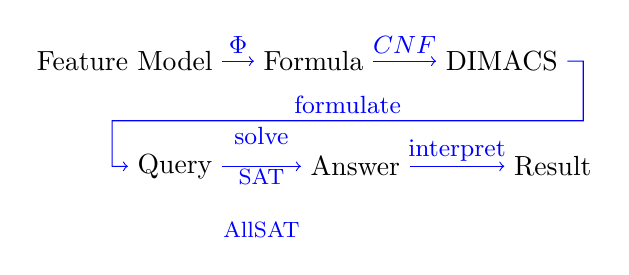
\begin{tikzpicture}
				\tikzset{block/.style={align=center,minimum height=5mm}}
				\node [block] (fm) {Feature Model};
				\node [block, right =4mm of fm] (formula) {Formula};
				\node [block, right =8mm of formula] (cnf) {DIMACS};
				\node [block, below right =8mm and -12mm of fm] (query) {Query};
				\node [block, right =10mm of query] (answer) {Answer};
				\node [block, right =12mm of answer] (result) {Result};
				\node [coordinate, below right =5mm and 2mm of cnf] (right) {};
				\node [coordinate, above left =3mm and 2mm of query] (left) {};
				\path[draw,->,color=blue] (fm) edge node[yshift=2mm] {\small $\Phi$} (formula)
							(formula) edge node[yshift=2mm] {\small $CNF$} (cnf)
							(cnf.east) -| (right) -- node[yshift=2mm] {\small formulate} (left) |- (query)
							(query) edge node[yshift=-2mm,align=center,font={\footnotesize}] {{\small solve}\\[1.5ex]SAT\\\ssat{}\\AllSAT} (answer)
							(answer) edge node [yshift=2mm]{\small interpret} (result);
			\end{tikzpicture}
		\end{definition}
		\begin{note}{}
			for brevity, we assume that $\phi = CNF(\Phi(FM))$ for a given feature model $FM$
		\end{note}
	\end{fancycolumns}
\end{frame}

% TODO I think I need a table here illustrating how the three different solvers can be combined with the three/four queries - to understand what comes next and in which order

\subsection{Consistency, Cardinality, and Enumeration}

\subsubsection{Feature Model}

\begin{frame}{\myframetitle}
	\begin{fancycolumns}[t]
		\emph{Consistency of Feature Models (SAT)}
		\begin{definition}{Void/Consistent Feature Model}
			\begin{itemize}
				\item are there grave modeling errors?
				\item is it possible to configure any product at all?
			\end{itemize}
			\centering
			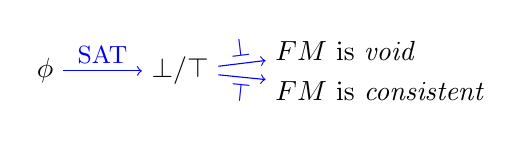
\begin{tikzpicture}
				\tikzset{block/.style={align=center,minimum height=5mm}}
				\node [block] (query) {$\phi$};
				\node [block, right =10mm of query] (answer) {$\bot/\top$};
				\node [block, above right =-3mm and 6mm of answer] (void) {$FM$ is \emph{void}};
				\node [block, below right =-3mm and 6mm of answer] (notvoid) {$FM$ is \emph{consistent}};
				\path[draw,->,color=blue] (query) edge node[yshift=2mm] {\small SAT} (answer)
							(answer) edge node [yshift=2mm,sloped]{\small $\bot$} (void)
							(answer) edge node [yshift=-2mm,sloped]{\small $\top$} (notvoid);
			\end{tikzpicture}
		\end{definition}
		\nextcolumn
		\emph{Cardinality of Feature Models (\ssat{})}
		\begin{definition}{How Many Products Are There?}
			\centering
			\begin{tikzpicture}
				\tikzset{block/.style={align=center,minimum height=5mm}}
				\node [block] (query) {$\phi$};
				\node [block, right =10mm of query] (answer) {$\abs{C}$};
				\path[draw,->,color=blue] (query) edge node[yshift=2mm] {\small \ssat{}} (answer);
			\end{tikzpicture}
		\end{definition}
		\begin{definition}{Variability Factor: Share of Products?}
			\centering
			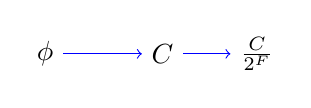
\begin{tikzpicture}
				\tikzset{block/.style={align=center,minimum height=5mm}}
				\node [block] (query) {$\phi$};
				\node [block, right =10mm of query] (answer) {$\abs{C}$};
				\node [block, right =6mm of answer] (num) {$\frac{\abs{C}}{2^{\abs{F}}}$};
				\path[draw,->,color=blue] (query) edge node[yshift=2mm] {\small \ssat{}} (answer)
							(answer) edge node [yshift=2mm,sloped]{} (num);
			\end{tikzpicture}
		\end{definition}
	\end{fancycolumns}
	\begin{fancycolumns}[t]
		\begin{exampletight}{}
			\begin{fancycolumns}[animation=none]
				\centering
				{\small\featureDiagram{Root,concrete[X,concrete,alternative][Y,concrete]}\\$\pnot (X \por Y)$}

				void
			\nextcolumn
				\centering
				{\small\featureDiagram{Root,concrete[X,concrete,alternative][Y,concrete]}\\$X \por Y$}

				consistent
			\end{fancycolumns}
		\end{exampletight}
		\nextcolumn
		\uncover<2->{\begin{exampletight}{}
			\begin{fancycolumns}[animation=none]
				\centering
				{\small\featureDiagram{Root,concrete[X,concrete,alternative][Y,concrete]}\\$\pnot (X \por Y)$}

				$0$ products, VF $0$
			\nextcolumn
				\centering
				{\small\featureDiagram{Root,concrete[X,concrete,alternative][Y,concrete]}\\$X \por Y$}

				$2$ products, VF $\frac{2}{8}$
			\end{fancycolumns}
		\end{exampletight}}
	\end{fancycolumns}
\end{frame}

\begin{frame}{\myframetitle}
	\begin{fancycolumns}[t]
		\emph{Feasibility of SAT-Based Analyses}

		\begin{note}{Is SAT-Based Analysis ``Easy''?}
			\begin{itemize}
				\item provocative claim: \mycite{SAT-based analysis of feature models is easy} \mysource{\href{https://dl.acm.org/doi/10.5555/1753235.1753267}{Mendonca~et~al.~2009}}
				\item easy $=$ performs much better than expected (although NP-complete)
				\item easy $=$ fast?
				\begin{itemize}
					\item what about formulating the query?\\
						(e.g., CNF transformation)
					\item what about many queries?\\
						(e.g., what we discuss next)
				\end{itemize}
			\end{itemize}
		\end{note}
	\nextcolumn
		\emph{Feasibility of \ssat{}-Based Analyses}
	
		\begin{exampletight}{Time to Count Products of Linux}
			\pic[width=\linewidth,page=4]{linux-plots}\\[-3mm]
			\begin{itemize}
				\item the solver from 2023 can solve models from 2003 % TODO which solver?
				\item can we analyze the models from 2023 in 2043?
			\end{itemize}
		\end{exampletight}
	\end{fancycolumns}
\end{frame}


\begin{frame}{\myframetitle}
	\begin{fancycolumns}
		\emph{Enumeration of Feature Models (AllSAT)}
		\begin{definition}{Which Products Are There?}
			\begin{itemize}
				\item \emph{P2(b)}: How to get all products?
			\end{itemize}
			\centering
			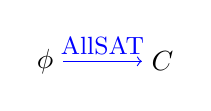
\begin{tikzpicture}
				\tikzset{block/.style={align=center,minimum height=5mm}}
				\node [block] (query) {$\phi$};
				\node [block, right =10mm of query] (answer) {$C$};
				\path[draw,->,color=blue] (query) edge node[yshift=2mm] {\small AllSAT} (answer);
			\end{tikzpicture}
		\end{definition}
		\begin{note}{}
			AllSAT does not scale to realistic feature models!\\
			50 features, configurations \`a 1 Byte $\approx$ 1 Petabyte
		\end{note} % TODO better example? what about the number of features such that it cannot be stored on all servers of the world? or we take a reasonable size of a hard disk in a notebook? 5 terrabyte? I (Thomas) cannot imagine a petabyte.
		\begin{exampletight}{}
			\begin{fancycolumns}[animation=none]
				\centering
				{\small\featureDiagram{Root,concrete[X,concrete,alternative][Y,concrete]}\\$\pnot (X \por Y)$}

				$\varnothing$
			\nextcolumn
				\centering
				{\small\featureDiagram{Root,concrete[X,concrete,alternative][Y,concrete]}\\$X \por Y$}

				$\{\{Root, X\},\{Root, Y\}\}$
			\end{fancycolumns}
		\end{exampletight}
	\nextcolumn
		\centering
		\sffamily
		\begin{tikzpicture}
			\tikzstyle{every edge}=[font=\tiny,draw,color=blue]

			\node (topleft) at (-1.4,0) {};
			\node (bottomleft) at (-1.4,-4) {};
			
			\node (fd) at (2,0) [align=center] {Feature Model\\[-1ex]{\tiny\color{lecturered}Feature Diagram, UVL}};
			\node (nat) at (0,-2) [align=center] {Natural Language\\[-1ex]{\tiny\color{lecturered}Thoughts, Plain Text}};
			\node (phi) at (2,-2) [align=center] {Formula\\[-1ex]{\tiny\color{lecturered}Infix Notation}};
			\node (cfg) at (4,-4) [align=center] {Configuration Map\\[-1ex]{\tiny\color{lecturered}Excel, Set of Sets}};
			\node (cnf) at (2,-4) [align=center] {CNF\\[-1ex]{\tiny\color{lecturered}DIMACS}};

			\path [dashed, thick, ->] (topleft) edge node[left, rotate=90, yshift=2mm, xshift=10mm] {Loss of Structure} (bottomleft);
		
			\path [->] (fd.south west) edge[bend left=15] node[sloped,yshift=1mm] {toString} (nat);
			\path [dotted, ->] (nat) edge[bend left=15] node[sloped,yshift=1mm] {} (fd.south west);
			
			\path [->] (fd.south) edge[bend left=15] node[sloped,yshift=1mm,rotate=90] {$\Phi$} (phi);
			\path [dotted, ->] (phi) edge[bend left=15] node[sloped,yshift=2mm,rotate=270] {} (fd.south);

			\path [->] (phi) edge[bend left=15] node[sloped,yshift=1mm] {CNF} (cnf);
			\path [dotted, ->] (cnf) edge[bend left=15] node[sloped,yshift=2mm,rotate=270] {} (phi);
		
			\path [->] (cfg) edge[bend right=15] node[sloped,yshift=1mm] {CNF} (cnf);
			\path [->] (cnf.south) edge[bend right=15] node[sloped,yshift=1mm] {AllSAT} (cfg);

			\node (trans) at (-1,-4.6) {};
			\node (trans2) at (2,-4.6) {};
			\node (trans3) at (-1,-4.9) {};
			\node (trans4) at (2,-4.9) {};
			\path [->] (trans) edge node[yshift=1mm] {Automated Transformation} (trans2);
			\path [dotted, ->] (trans3) edge[yshift=5mm] node[yshift=1mm] {Semi-Automated Transformation} (trans4);
		
			\node (bottomleft2) at (-0.2,-5) {\tiny\color{lecturered}Concrete Format};
		\end{tikzpicture} % TODO position of "Concrete Format" not optimal. gray out irrelevant parts? not sure what to look at here.
	\end{fancycolumns}
\end{frame}

\subsubsection{Features}

\begin{frame}{\myframetitle}
	\begin{fancycolumns}[t]
		\emph{Consistency of Features (SAT)}
		\begin{definition}{Core/Dead Feature}
			\begin{itemize}
				\item can a feature $F$ be (de-)selected at all?
			\end{itemize}
			\centering
			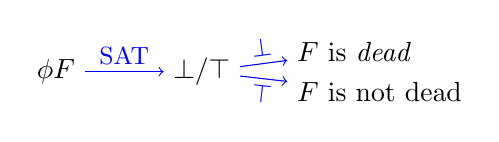
\begin{tikzpicture}
				\tikzset{block/.style={align=center,minimum height=5mm}}
				\node [block] (query) {$\phi \pand F$};
				\node [block, right =10mm of query] (answer) {$\bot/\top$};
				\node [block, above right =-3mm and 6mm of answer] (void) {$F$ is \emph{dead}};
				\node [block, below right =-3mm and 6mm of answer] (notvoid) {$F$ is not dead};
				\path[draw,->,color=blue] (query) edge node[yshift=2mm] {\small SAT} (answer)
							(answer) edge node [yshift=2mm,sloped]{\small $\bot$} (void)
							(answer) edge node [yshift=-2mm,sloped]{\small $\top$} (notvoid);
			\end{tikzpicture}
			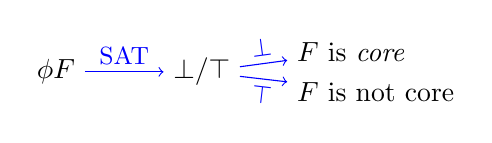
\begin{tikzpicture}
				\tikzset{block/.style={align=center,minimum height=5mm}}
				\node [block] (query) {$\phi \pand \pnot F$};
				\node [block, right =10mm of query] (answer) {$\bot/\top$};
				\node [block, above right =-3mm and 6mm of answer] (void) {$F$ is \emph{core}};
				\node [block, below right =-3mm and 6mm of answer] (notvoid) {$F$ is not core};
				\path[draw,->,color=blue] (query) edge node[yshift=2mm] {\small SAT} (answer)
							(answer) edge node [yshift=2mm,sloped]{\small $\bot$} (void)
							(answer) edge node [yshift=-2mm,sloped]{\small $\top$} (notvoid);
			\end{tikzpicture}
		\end{definition}
		\nextcolumn
		\emph{Cardinality of Features (\ssat{})}
		\begin{definition}{How Many Products Include Feature $F$?}
			\centering
			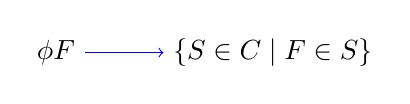
\begin{tikzpicture}
				\tikzset{block/.style={align=center,minimum height=5mm}}
				\node [block] (query) {$\phi \pand F$};
				\node [block, right =10mm of query] (answer) {$\abs{\{S \in C \mid F \in S\}}$};
				\path[draw,->,color=blue] (query) edge node[yshift=2mm] {\small \ssat{}} (answer);
			\end{tikzpicture}
		\end{definition}
		\begin{definition}{Commonality: How Constrained is This Feature?}
			\centering
			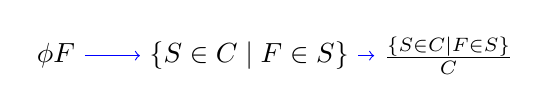
\begin{tikzpicture}
				\tikzset{block/.style={align=center,minimum height=5mm}}
				\node [block] (query) {$\phi \pand F$};
				\node [block, right =7mm of query] (answer) {$\abs{\{S \in C \mid F \in S\}}$};
				\node [block, right =2mm of answer] (num) {$\frac{\abs{\{S \in C \mid F \in S\}}}{\abs{C}}$};
				\path[draw,->,color=blue] (query) edge node[yshift=2mm] {\small \ssat{}} (answer)
							(answer) edge node [yshift=2mm,sloped]{} (num);
			\end{tikzpicture}
		\end{definition}
	\end{fancycolumns}
	\begin{fancycolumns}[t]
		\begin{exampletight}{}
			\centering
			{\small\featureDiagram{Root,concrete[X,concrete,alternative][Y,concrete]}\\$\pnot X$}

			$X$ is dead\hfill$Root$ and $Y$ are core
		\end{exampletight}
		\nextcolumn
		\begin{exampletight}{}
			\centering
			{\small\featureDiagram{Root,concrete[X,concrete,alternative][Y,concrete]}\\$\pnot X$}

			$X$: 0 products\hfill$Root$ and $Y$: 1 products
		\end{exampletight}
	\end{fancycolumns}
\end{frame}

\subsubsection{Partial Configurations}

\begin{frame}{\myframetitle}
	\begin{fancycolumns}[t]
		\emph{Consistency of Partial Configurations (SAT)}
		\begin{definition}{Valid Partial Configuration}
			Is a partial configuration $C = ({\color{lecturegreen}S}, {\color{lecturered}D})$ consistent with the feature model? % TODO would be easier if term valid could be used here

			\centering
			\begin{tikzpicture}
				\tikzset{block/.style={align=center,minimum height=5mm}}
				\node [block] (query) {$\phi \pand \bigwedge_{s \in S} {\color{lecturegreen}s} \pand \bigwedge_{d \in D} {\color{lecturered}\pnot d}$};
				\node [block, right =10mm of query] (answer) {$\bot/\top$};
				\node [block, above right =-3mm and 6mm of answer] (void) {$C$ $\times$};
				\node [block, below right =-3mm and 6mm of answer] (notvoid) {$C$ \checkmark};
				\path[draw,->,color=blue] (query) edge node[yshift=2mm] {\small SAT} (answer)
							(answer) edge node [yshift=2mm,sloped]{\small $\bot$} (void)
							(answer) edge node [yshift=-2mm,sloped]{\small $\top$} (notvoid);
			\end{tikzpicture}
		\end{definition}
		\nextcolumn
		\emph{Cardinality of Partial Configurations (\ssat{})}
		\begin{definition}{How Many Products Are Still Configurable for $C$?}
			\centering
			\begin{tikzpicture}
				\tikzset{block/.style={align=center,minimum height=5mm}}
				\node [block] (query) {$\phi \pand ...$};
				\node [block, right =10mm of query] (answer) {$\abs{\{(S', D') \in C \mid {\color{lecturegreen}S} \subseteq S', {\color{lecturered}D} \in D'\}}$};
				\path[draw,->,color=blue] (query) edge node[yshift=2mm] {\small \ssat{}} (answer);
			\end{tikzpicture}
		\end{definition}
	\end{fancycolumns}
	\begin{fancycolumns}[t]
		\begin{exampletight}{}
			\centering
			{\small\featureDiagram{Root,concrete[X,concrete,optional][Y,concrete,optional]}\\$X \pimplies Y$}

			\cfg{Root}{X} \checkmark
		\end{exampletight}
		\nextcolumn
		\begin{exampletight}{}
			\centering
			{\small\featureDiagram{Root,concrete[X,concrete,optional][Y,concrete,optional]}\\$X \pimplies Y$}

			\cfg{Root}{X}: 2 products
		\end{exampletight}
	\end{fancycolumns}
\end{frame}

\subsection{Automated Analyses in FeatureIDE}

\subsubsection*{Feature-Model Editor}

\begin{frame}{\myframetitle}
	\begin{fancycolumns}[widths={60,40}]
		\begin{exampletight}{} % TODO would be great to show an explanation here
			\picDark[width=\textwidth]{featureide-feature-model-editor-waffle}
		\end{exampletight}
	\nextcolumn
		\begin{exampletight}{}
			\picDark[width=\textwidth]{featureide-feature-model-statistics}
		\end{exampletight}
	\end{fancycolumns}
\end{frame}

\subsubsection*{Configuration Editor}

\begin{frame}{\myframetitle}
	\begin{fancycolumns}[widths={60,40}]
		\begin{exampletight}{}
			\centering
			\picDark[width=.27\textwidth]{featureide-configuration-editor-step1}
			$\Rightarrow$
			\picDark[width=.63\textwidth]{featureide-configuration-editor-step2}
		\end{exampletight}
	\nextcolumn
		\begin{note}{Decision Propagation}
			\begin{itemize}
				\item after each decision (i.e., click) \ldots
				\begin{itemize}
					\item \ldots{} select features that are now \emph{conditionally core}
					\item \ldots{} deselect features that are now \emph{conditionally dead}
				\end{itemize}
				\item this way it is impossible to configure an invalid configuration
				\item explanations for all propagated decisions
			\end{itemize}
		\end{note}
	\end{fancycolumns}
\end{frame}

\begin{frame}{Automated Analysis of Feature Models}
	\begin{fancycolumns}
		\begin{definition}{The Road So Far \ldots}
			\centering
			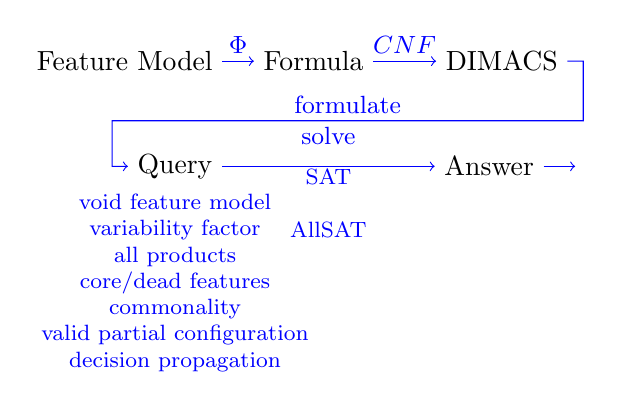
\begin{tikzpicture}
				\tikzset{block/.style={align=center,minimum height=5mm}}
				\node [block] (fm) {Feature Model};
				\node [block, right =4mm of fm] (formula) {Formula};
				\node [block, right =8mm of formula] (cnf) {DIMACS};
				\node [block, below right =8mm and -12mm of fm] (query) {Query};
				\node [block, below =-.5mm of query,align=center,color=blue,font={\footnotesize}] (query2) {void feature model\\variability factor\\all products\\core/dead features\\commonality\\valid partial configuration\\decision propagation};
				\node [block, right =27mm of query] (answer) {Answer};
				\node [block, right =4mm of answer] (result) {};
				\node [coordinate, below right =5mm and 2mm of cnf] (right) {};
				\node [coordinate, above left =3mm and 2mm of query] (left) {};
				\path[draw,->,color=blue] (fm) edge node[yshift=2mm] {\small $\Phi$} (formula)
							(formula) edge node[yshift=2mm,align=center] {\small $CNF$} (cnf)
							(cnf.east) -| (right) -- node[yshift=2mm] {\small formulate} (left) |- (query)
							(query) edge node[yshift=-2mm,align=center,font={\footnotesize}] {{\small solve}\\[1.5ex]SAT\\\ssat{}\\AllSAT} (answer)
							(answer) edge (result);
			\end{tikzpicture}
		\end{definition}
	\nextcolumn
		\begin{definition}{\ldots\ and Beyond}
			\centering
			\begin{tikzpicture}
				\tikzset{block/.style={align=center,minimum height=5mm}}
				\node [block,align=center,color=lecturered,font={\footnotesize}] (fm2) {attributes\\cardinalities\\submodels};
				\node [block, below =.5mm of fm2] (fm) {Feature Model};
				\node [block, right =4mm of fm] (formula) {Formula};
				\node [block, above =.5mm of formula,align=center,color=lecturered,font={\footnotesize}] (formula2) {quantifiers\\predicates\\functions};
				\node [block, right =8mm of formula] (cnf) {DIMACS};
				\node [block, above =.5mm of cnf,align=center,color=lecturered,font={\footnotesize}] (cnf2) {DNF\\d-DNNF\\BDD};
				\node [block, below right =8mm and -12mm of fm] (query) {Query};
				\node [block, below =-.5mm of query,align=center,color=lecturered,font={\footnotesize}] (query2) {false-optional features\\atomic sets\\redundant constraints\\feature-model edits\\explanations\\sampling\\slicing};
				\node [block, right =27mm of query] (answer) {Answer};
				\node [block, right =4mm of answer] (result) {};
				\node [coordinate, below right =5mm and 2mm of cnf] (right) {};
				\node [coordinate, above left =3mm and 2mm of query] (left) {};
				\path[draw,->,color=blue] (fm) edge node[yshift=2mm] {\small $\Phi$} (formula)
							(formula) edge node[yshift=0mm,align=center] {\small $CNF$\\{\footnotesize\color{lecturered}Tseitin}} (cnf)
							(cnf.east) -| (right) -- node[yshift=2mm] {\small formulate} (left) |- (query)
							(query) edge node[yshift=-7mm,align=center,font={\footnotesize}] {{\small solve}\\[1.5ex]SAT, \ssat{}, AllSAT\\{\color{lecturered}MAX-SAT}\\{\color{lecturered}Solution-SAT}\\{\color{lecturered}MUS}\\{\color{lecturered}SMT, CSP}\\{\color{lecturered}QBF}\\{\color{lecturered}WMC, PMC}} (answer)
							(answer) edge (result);
			\end{tikzpicture}
			\vspace*{-3ex}
			\begin{itemize}
				\item develop new analyses
				\item improve efficiency of existing analyses
				\item investigate correctness and compositionality
			\end{itemize}
		\end{definition}
	\end{fancycolumns}
\end{frame}
\lessonslearned{
	\item with solvers, we can build reliable configurators for product lines
	\item SAT-based analyses: void feature model, core/dead features, decision propagation
	\item \ssat{}-based analyses: variability factor, feature commonality
}{ % TODO unify literature pointer (see Lecture 1-3)
	\item \fospl\mysection{10.1}\mypages{244--254}\\--- introduction to feature-model analysis
	\item David Benavides et al. (2010): \href{https://doi.org/10.1016/j.is.2010.01.001}{Automated Analysis of Feature Models 20 Years Later: A Literature Review}\\--- old but extensive literature survey
	\item Chico Sundermann et al. (2021): \href{https://doi.org/10.1145/3442391.3442404}{Applications of \#SAT Solvers on Feature Models}\\--- experiments on the scalability of \ssat{} solvers % TODO replace by EMSE paper?
	% TODO we could add the paper about web configurators here
}{
	\begin{center}
		\featureDiagramABCDE
	\end{center}

	think of a constraint that would make exactly one feature dead
%	How can you \ldots
%	\begin{enumerate}
%		\item make this feature model void
%		\item make exactly one feature dead
%	\end{enumerate}
%	\ldots{} by adding one constraint, respectively?
%
%	Name a partial configuration for which only two products exist.
}

\faq{
	\item What is feature modeling? When is it needed?
	\item How can we specify valid combinations of features?
	\item What is a complete, partial, valid, invalid configuration?
	\item What are (dis-)advantages of natural language, configuration map, and feature models?
	\item What is the graphical syntax and semantics of feature models?
	\item Give an example feature model!
}{
	\item What representations of feature models are available? Are they equivalent?
	\item How to represent feature models textually?
	\item What is UVL (used for)?
	\item How to identify whether a configuration is valid?
	\item How to translate feature model into a propositional formula?
	\item What are DIMACS and KConfig (used for)?
	\item Would you recommend Excel for feature model? Why (not)?
}{
	\item Why can configuration become challenging?
	\item How can we identify problems with feature models and configurations?
	\item How can feature models by analyzed? What analyses are available?
	\item What solvers can be used to analyze feature models?
	\item What is the difference between SAT, \ssat, and ALLSAT?
	\item Why are solvers useful when creating configurations?
}

\mode<beamer>{
	\addtocounter{framenumber}{-1}
	\begin{frame}{\inserttitle}
		\lectureseriesoverview[\insertlecturenumber]
	\end{frame}

	%\addtocounter{framenumber}{-1}
	%\againtitle % TODO does not work as we have redefined maketitle
}


% TODO L05 CONDITIONAL COMPILATION

\ifuniversity{recording}{\date{April 23, 2023}\setpicture[75]{may21-north2}\setcopyright{}}
\ifuniversity{ulm}{\date{May 11, 2023}\setpicture[75]{may21-north2}}
\ifuniversity{magdeburg}{\setpicture[300]{magdeburg-river}\setcopyright{}}
\ifuniversity{bern}{\setpicture[10]{unibe_00213_200601_1200}}
\ifuniversity{paderborn}{\date{May 15, 2024}\setpicture[150]{image10}}
\ifuniversity{braunschweig}{\date{November 13, 2024}}

\author{Thomas Thüm, Elias Kuiter, Timo Kehrer}
\lecture{Conditional Compilation}{conditional}

% TODO we should use conditional compilation with build systems (preprocessors) instead. would require numerous changes in this lecture. problem is that conditional compilation is currently introduced in Part II only, which needs to be somehow moved to Part I then.
\section{Features with Build Systems}
\subsection{How to Implement Features?}
\begin{frame}[label=HowToImplementFeatures]{\myframetitle}
	\begin{fancycolumns}
		\begin{exampletight}{Given a feature model for graphs \ldots}
			\centering\featureDiagramGraphs
		\end{exampletight}
		\begin{example}{\ldots\ we can derive a valid configuration}
			\small
			\begin{fancycolumns}[columns=3,animation=none]
				$\{G\}$\\
				$\{G,C\}$\\
				$\{G,D\}$\\
				$\{G,C,D\}$\\
			\nextcolumn
				$\{G,W\}$\\
				$\{G,C,W\}$\\
				$\{G,D,W\}$\\
				$\{G,C,D,W\}$\\
			\nextcolumn
				$\{G,W,S\}$\\
				$\{G,C,W,S\}$\\
				$\{G,D,W,S\}$\\
				$\{G,C,D,W,S\}$\\
			\end{fancycolumns}
		\end{example}
	\nextcolumn
		\begin{exampletight}{How to Generate Products Automatically?}
			\centering\foreach \page in {2,12,4,14,6,16,8,18,10,20,42,44}{\mbox{~\pic[width=.175\linewidth,page=\page]{graphs}~} }
		\end{exampletight}
		\begin{note}{Goals}
			\begin{itemize}
				\item descriptive specification of a product (i.e., a configuration, a selection of features)
				\item automated generation of a product with compile-time variability
			\end{itemize}
			Focus of \lecturefeatures\ --\ \lecturelanguages
		\end{note}
	\end{fancycolumns}
\end{frame}

\subsection{Problems of Ad-Hoc Approaches for Variability}

\subsubsection{Features with Runtime Variability?}
\againframe<2>{GraphWithGlobalVariables}

\begin{frame}[label=SPLwithPreferenceDialogsCommandLineOptionsConfigurationFiles]{\myframetitle}
	\begin{fancycolumns}[b,widths={36}]
		\picDark[width=\linewidth]{preferences-eclipse}

		\begin{definition}{How to? -- Preference Dialog}
			\begin{itemize}
				\item implement runtime variability
				\item compile the program
				\item run the program
				\item \emph{manually adjust preferences based on configuration}
			\end{itemize}
		\end{definition}
	\nextcolumn
		\begin{fancycolumns}[widths={41},animation=none]
			\pic[width=\linewidth]{runtime-parameters-win10-cmd-dir}
		\nextcolumn
			\picDark[width=\linewidth]{configfile-eclipse-ini}
		\end{fancycolumns}

		\begin{definition}{How to? -- Command-Line Options / Configuration Files}
			\begin{itemize}
				\item implement runtime variability
				\item compile the program
				\item \emph{automatically generate command-line options / configuration files based on configuration}
				\item run the program
			\end{itemize}
		\end{definition}
	\end{fancycolumns}
\end{frame}

\begin{frame}[fragile,label=SPLwithImmutableGlobalVariables]{\myframetitle}
	\begin{fancycolumns}[widths={48}]
\begin{codetight}[basicstyle=\small]{}
public class Config {
	~public final static boolean COLORED = true;~
	@public final static boolean WEIGHTED = false;@
}
\end{codetight}
		\begin{definition}{How to? -- Immutable Global Variables}
			\begin{itemize}
				\item implement runtime variability
				\item \emph{automatically generate class with global variables based on configuration}
				\item compile and run the program
			\end{itemize}
		\end{definition}
	\nextcolumn
		\begin{note}{What is missing?}
			\begin{itemize}
				\item automated generation:\\\hfill for preference dialogs
				\item no compile-time variability / same large binary:\\\hfill for all except immutable global variables
				\item very limited compile-time variability:\\\hfill for immutable global variables
			\end{itemize}
		\end{note}
	\end{fancycolumns}
\end{frame}

\subsubsection{Features with Clone-and-Own?}
\begin{frame}[label=SPLwithCloneAndOwn]{\myframetitle}
	\begin{fancycolumns}[widths={30},animation=none]
		\centering~

		\picDark[scale=0.2]{alice}
		\pic[scale=0.26,page=2]{graphs}

		\picDark[scale=0.2]{bob}
		\pic[scale=0.26,page=12]{graphs}

		\picDark[scale=0.2]{eve}
		\pic[scale=0.26,page=16]{graphs}
	\nextcolumn
		\begin{definition}{How to?}
			\begin{itemize}
				\item implement separate project for each product\\(i.e., branch with version control)
				\item download project / checkout branch based on configuration
				\item run build script, if existent
				\item compile and run the program
			\end{itemize}
		\end{definition}
		\pause
		\begin{note}{What is missing?}
			\begin{itemize}
				\item compile-time variability only for implemented products
				\item no automated generation:\\\hfill for clone-and-own (with version control systems)
				\item automated generation based on build script and extra files:\\\hfill for clone-and-own with build systems
				\item no free feature selection (i.e., configuration)
			\end{itemize}
		\end{note}
	\end{fancycolumns}
\end{frame}

\subsection{Recap: Clone-and-Own with Build Systems}
\begin{frame}{\myframetitle\  \mytitlesource{\href{https://dl.acm.org/doi/10.1145/3461002.3473950}{Kuiter~et~al.~2021}}}
	\begin{fancycolumns}[columns=2,widths={76},animation=none]
		\begin{fancycolumns}[widths={50},animation=none] % TODO widths needed due to bug #56 in slide template
			\begin{example}{Case Study: Anesthesia Device}
				\begin{itemize}
					\item C application
					\item targets embedded devices (ESP32)
					\item configurations are hard-coded as build scripts
				\end{itemize}
			\end{example}
		\nextcolumn
			\uncover<4->{
				\begin{exampletight}{{\color{lecturered}Production Device}: OLED, Clock}
					\centering\pic[height=25mm]{pignap-cfg-production-oled}
				\end{exampletight}
			}
		\end{fancycolumns}
		\begin{fancycolumns}[widths={50},animation=none] % TODO widths needed due to bug #56 in slide template
			\uncover<2->{
				\begin{exampletight}{{\color{lecturegreen}Prototype}: OLED Display}
					\centering\pic[height=25mm]{pignap-cfg-prototype-oled}
				\end{exampletight}
			}
		\nextcolumn
			\uncover<3->{
				\begin{exampletight}{{\color{lectureblue}Prototype}: LCD, Real-Time Clock}
					\centering\pic[height=25mm]{pignap-cfg-prototype-lcd-rtc}
				\end{exampletight}
			}
		\end{fancycolumns}
	\nextcolumn
		\only<1|handout:0>{\pic[width=\linewidth,page=1]{pignap-variants}}%
		\only<2|handout:0>{\pic[width=\linewidth,page=2]{pignap-variants}}%
		\only<3|handout:0>{\pic[width=\linewidth,page=3]{pignap-variants}}%
		\only<4->{\pic[width=\linewidth,page=4]{pignap-variants}}
	\end{fancycolumns}
\end{frame}

\subsection{Introducing Features to Build Systems}
\begin{frame}[label=SPLwithBuildSystems]{\myframetitle\  \mytitlesource{\href{https://dl.acm.org/doi/10.1145/3461002.3473950}{Kuiter~et~al.~2021}}}
	\begin{fancycolumns}[widths={60}]
		\begin{definition}{How to Implement Features with Build Systems?}
			\begin{itemize}
				\item step 1: model variability in a feature model
				\item step 2: in build scripts, in- and exclude files based on feature selection
				\item step 3: pass a feature selection at build time
			\end{itemize}
			$\Rightarrow$ one build script per group of related features
		\end{definition}
		\begin{center}
			\featureDiagram{Anesthesia Device,abstract
			[Monitoring,abstract,mandatory
				[Display,abstract,or[LCD,concrete,alternative][OLED,concrete]]
				[Wi-Fi,abstract
					[HTTP Server,concrete,mandatory]]]
			[History,optional,concrete]
			[Libraries,abstract,mandatory
				[Storage,abstract,optional[NVS,concrete,alternative][FRAM,concrete]]
				[RTC,concrete,optional[Battery,concrete,mandatory]]]}

			$History \pimplies Storage \pand RTC$
		\end{center}
	\nextcolumn
		\centering\pic[height=\textheightwithtitle]{pignap-features}
	\end{fancycolumns}
\end{frame}

\subsection{The Linux Kernel}

\xkcdframe{619} % linux features 20s

\subsubsection*{KConfig for Feature Modeling}

\begin{frame}[fragile]{\myframetitle}
	\begin{fancycolumns}
		\begin{kconfigtight}[basicstyle=\small]{Part of the x86 Architecture \mysource{\href{https://github.com/torvalds/linux/blob/0326074/arch/x86/Kconfig}{linux/arch/x86/Kconfig}}}
config 64BIT
	bool "64-bit kernel" if "$(ARCH)" = "x86"
	default "$(ARCH)" != "i386"
	help
		Say yes to build a 64-bit kernel (x86_64)
		Say no to build a 32-bit kernel (i386)

config X86_32
	def_bool y
	depends on !64BIT
	# Options that are inherently 32-bit kernel only:
	select GENERIC_VDSO_32
	select ARCH_SPLIT_ARG64

config X86_64
	def_bool y
	depends on 64BIT
	# Options that are inherently 64-bit kernel only:
	select ARCH_HAS_GIGANTIC_PAGE
	select ARCH_SUPPORTS_INT128 if CC_HAS_INT128
\end{kconfigtight}
	\nextcolumn
		\begin{definition}{KConfig Language\mysource{\href{https://www.kernel.org/doc/html/latest/kbuild/kconfig-language.html}{kernel.org}}}
			\begin{itemize}
				\item configuration language used in embedded/OS development (e.g., Linux, Zephyr, ESP32)
				\item similar to UVL, but has many quirks (e.g., tristate features, \texttt{select})
				\item transformation into formula or feature model possible, but not trivial \mysource{\href{https://dl.acm.org/doi/abs/10.1145/3468264.3468578}{Oh~et~al.~2021}}
			\end{itemize}
		\end{definition}
		\hspace*{-0.07253886\linewidth}%=2*0.035/(1-0.035)
		\linuxbddlink{\pic[width=1.3\linewidth,trim=220 510 60 180,clip]{2020/2020-SPLC-Thuem}}
	\end{fancycolumns}
\end{frame}

\subsubsection*{MenuConfig for Configuration}

\begin{frame}{\myframetitle}
	\begin{fancycolumns}[widths={60,40}]
		\begin{exampletight}{}
			\pic[width=\textwidth]{linux-menuconfig} % sudo apt install make flex bison libncurses5-dev && make menuconfig
		\end{exampletight}
	\nextcolumn
		\begin{note}{make menuconfig}
			\begin{itemize}
				\item configures KConfig models
				\item generates a \texttt{.config} file
				\item widely used to configure Linux
				\item still: it is possible to create invalid configurations and products % TODO does not fit into the storyline anymore. remove?
			\end{itemize}
		\end{note}
	\end{fancycolumns}
\end{frame}

\subsubsection*{KBuild as Build System}

\begin{frame}[fragile,t]{\myframetitle}
	\vspace*{-2ex}
	\begin{fancycolumns}[t]
		\begin{kconfigtight}[basicstyle=\footnotesize]{Feature Model with KConfig\mysource{\href{https://github.com/torvalds/linux/blob/0326074/arch/x86/Kconfig}{linux/arch/x86/Kconfig}}}
config X86_32 ...
config X86_64 ...

config IA32_EMULATION
	bool "IA32 Emulation"
	depends on X86_64
	help Include code to run legacy 32-bit programs under a 64-bit kernel. You should likely enable this, unless you're 100% sure that you don't have any 32-bit programs left.
\end{kconfigtight}
		\begin{definition}{KBuild\mysource{\href{https://www.kernel.org/doc/html/latest/kbuild/makefiles.html}{kernel.org}}}
			\begin{itemize}
				\item a style for writing Makefiles in Linux
				\item defines goals with Make variables
				\begin{itemize}
					\small
					\item \texttt{obj-y} ($\approx 8\%$): static linkage (= include feature)
					\item \texttt{obj-m} ($< 1\%$): dynamic linkage (= as module)
					\item \texttt{obj-} ($0\%$): no linkage (= exclude feature)
					\item \texttt{obj-\$(\ldots)} ($\approx 91\%$): conditional compilation
				\end{itemize}
				\item full power of Make $\Rightarrow$ hard to comprehend
			\end{itemize}
		\end{definition}
	\nextcolumn
		\begin{onlyenv}<2|handout:0>
			\begin{kbuildtight}[basicstyle=\small]{Feature Mapping with KBuild \mysource{\href{https://github.com/torvalds/linux/blob/0326074/arch/x86/Kbuild}{linux/arch/x86/Kbuild}}}
# link these subdirectories statically:
obj-y += entry/ # entry routines
obj-y += realmode/ # 16-bit support
obj-y += kernel/ # x86 kernel
obj-y += mm/ # memory management

# link these depending on a configuration option:
obj-~$(CONFIG_IA32_EMULATION)~ += ia32/
obj-~$(CONFIG_XEN)~ += xen/ # paravirtualization


obj-~$(CONFIG_HYPERV)~ += hyperv/
			\end{kbuildtight}
		\end{onlyenv}
		\begin{uncoverenv}<3-|handout:1>
			\begin{kbuildtight}[basicstyle=\small]{Feature Mapping with KBuild \mysource{\href{https://github.com/torvalds/linux/blob/0326074/arch/x86/Kbuild}{linux/arch/x86/Kbuild}}}
# link these subdirectories statically:
obj-y += entry/ # entry routines
obj-y += realmode/ # 16-bit support
obj-y += kernel/ # x86 kernel
obj-y += mm/ # memory management

# link these depending on a configuration option:
obj-~$(CONFIG_IA32_EMULATION)~ += ia32/
obj-~$(CONFIG_XEN)~ += xen/ # paravirtualization

# in the real code, kconfig is (unintuitively?) overridden:
obj-~$(subst m,y,$(CONFIG_HYPERV))~ += hyperv/
			\end{kbuildtight}
		\end{uncoverenv}
		\begin{uncoverenv}<4-|handout:1>
			\begin{kbuildtight}[basicstyle=\small]{Recurse into Subsystems\mysource{\href{https://github.com/torvalds/linux/blob/0326074/arch/x86/ia32/Makefile}{linux/arch/x86/ia32/Makefile}}}
# ia32 kernel emulation subsystem
obj-~$(CONFIG_IA32_EMULATION)~ := ia32_signal.o
audit-class-~$(CONFIG_AUDIT)~ := audit.o

# IA32_EMULATION and AUDIT required for audit.o:
obj-~$(CONFIG_IA32_EMULATION)~ += ~$(audit-class-y)~
			\end{kbuildtight}
		\end{uncoverenv}
	\end{fancycolumns}
\end{frame}

\begin{frame}[fragile]{\myframetitle}
	\begin{fancycolumns}
		\begin{example}{Interactive Linux Kernel Configurator}
			\pic[width=\linewidth]{linux-menuconfig-emulation}
		\end{example}

		\begin{kconfigtight}[basicstyle=\footnotesize]{Feature Model and Example Configuration}
			config AUDIT ... # configured as NO
			config IA32_EMULATION ... # configured as YES
			config HYPERV ... # configured as MODULE
			config XEN ... # configured as NO
\end{kconfigtight}
	\nextcolumn
		\begin{kbuildtight}[basicstyle=\small]{Feature Mapping}
obj-y += entry/ realmode/ kernel/ mm/
obj-~$(CONFIG_IA32_EMULATION)~ += ia32/
obj-~$(CONFIG_XEN)~ += xen/
obj-~$(subst m,y,$(CONFIG_HYPERV))~ += hyperv/
obj-~$(CONFIG_IA32_EMULATION)~ := ia32_signal.o
audit-class-~$(CONFIG_AUDIT)~ := audit.o
obj-~$(CONFIG_IA32_EMULATION)~ += ~$(audit-class-y)~
		\end{kbuildtight}

		\begin{kbuildtight}[basicstyle=\small]{Feature Mapping for Example Configuration}
obj-y += entry/ realmode/ kernel/ mm/
obj-?y? += ia32/
obj- += xen/
obj-?y? += hyperv/
obj-?y? := ia32_signal.o
audit-class- := audit.o
obj-?y? +=
		\end{kbuildtight}

		\begin{note}{}
			\small i.e., \texttt{entry, realmode, kernel, mm, ia32, hyperv, ia32\_signal.o} are compiled
		\end{note}
	\end{fancycolumns}
\end{frame}

% TODO add quote? \mycite{As Kbuild relies on a Turing-complete language, complex conditions can be encoded.} \mysource{\fospl\mypage{108}}

\subsection{Discussion}
\newcommand{\MajorChallengesOfBuildSystems}{
	\item build scripts may become complex, there is no limit to what can be done (e.g., you can run arbitrary shell commands on files)\\
		$\Rightarrow$ \emph{hard to understand and analyze}
	\item no simple inclusion and exclusion of individual lines or chunks of code\\
	$\Rightarrow$ high-level use \emph{only}!
}
\begin{frame}<1-2>[label=DiscussionOfBuildSystems]
	\frametitle<1-2>{Discussion of Features with Build Systems}
	\frametitle<3>{\myframetitle}
	\begin{fancycolumns}
		\begin{note}{Advantages}
			\begin{itemize}
				\item compile-time variability\\
					$\Rightarrow$ \emph{fast, small binaries} with smaller attack surface and without disclosing secrets
				\item automated generation of arbitrary products\\
					$\Rightarrow$ \emph{free feature selection}
				\item allows in- and exclusion of individual files or even entire subsystems\\
					$\Rightarrow$ high-level, \emph{modular variability}
			\end{itemize}
		\end{note}
	\nextcolumn
		\begin{note}{Challenges}
			\begin{itemize}
				\item not reconfigurable at run- or load-time % this challenge is not relevant on subsequent slides
				\MajorChallengesOfBuildSystems
			\end{itemize}
		\end{note}
	\end{fancycolumns}
\end{frame}

\lessonslearned{
	\item ad-hoc variability is lacking
	\item features with build systems allow for automated generation of products and free feature selection
	\item build systems include entire files, not lines or chunks
}{
	\item \fospl\mychapter{5.2.1}\mypages{105--106}\\--- brief introduction to variability in build scripts
	% TODO add literature? van der Storm T (2004).Variability and component composition. In: Proc. Int’l Conf. Software Reuse (ICSR) Lecture notes in computer science, vol 3107. Springer, pp 157–166
	\item \fospl\mychapter{5.2.3}\mypages{107--108}\\--- variability in build scripts of the Linux kernel
	% TODO add literature? Berger T, She S, Czarnecki K, Wa ̨sowski A (2010a) Feature-to-code mapping in two large product lines. In: Proc. Int’l Software Product Line Conference (SPLC). Lecture Notes in Computer Science, vol 6287. Springer, pp 498–499
	% TODO add literature? Dietrich C, Tartler R, Schröder-Preikschat W, Lohmann D (2012b) Understanding Linux feature distribution. In: Proc. AOSD Workshop on Modularity In Systems Software (MISS). ACM Press, pp 15–20
	% TODO add work on KernelHaven
}{
% example replaced, as this is probably better for the actual exercise
%	Choose a build system and sketch how it may be used to implement this SPL (file structure and build script):
%
%	\begin{center}
%		\small\featureDiagramConfigurableDatabase
%	\end{center}
	\begin{enumerate}
		\item[] What are differences of the following two implementation techniques for variability?
			\begin{enumerate}
				\item[(a)] clone-and-own with build systems
				\item[(b)] features with build systems
			\end{enumerate}
		% TODO removed the next task, as the term granularity has not been defined yet
		%\item What is the respective granularity?
	\end{enumerate}

	\uploadpractice
}

\section{Features with Preprocessors}
% TODO add this paper? https://www.sciencedirect.com/science/article/pii/S0950584916300921
% TODO add examples for undisciplined ifdefs? https://dl.acm.org/doi/abs/10.1145/1960275.1960299

\subsection{Granularity of Variability}
\begin{frame}{\myframetitle}
	\begin{fancycolumns}[animation=none]
		\begin{definition}{Granularity of Variability}
			\begin{itemize}
				\item Depending on the implementation technique, variability can be introduced at different levels of granularity.
				\item A level of granularity refers to
				\begin{itemize}
					\item the hierarchical organization of implementation artifacts (e.g., through the file system),
					\item the hierarchical structure of an implementation artifact (e.g., given by its syntax)
				\end{itemize}
			\end{itemize}
		\end{definition}
		\begin{example}{Granularity Levels in Java}
			modules $>$ libraries $>$ packages $>$ classes $>$ members $>$ statements $>$ parameters
		\end{example}
		\pause
	\nextcolumn
		\begin{note}{What we have seen so far?}
			\begin{itemize}
				\item Coarse-grained: Clone-and-own with version control (entire variants)
				\item Medium-grained: Clone-and-own with build systems (file level)
				\item Medium-grained: Features with build systems (file level)
				\item Medium-grained: Design patterns for variability (class or member level)
				\item Fine-grained: Runtime parameters (statement level) 
			\end{itemize}
		\end{note}
		\pause
		\begin{note}{What is missing?}
			Yet no approach supporting fine-grained compile-time variability!
		\end{note}		
	\end{fancycolumns}
\end{frame}
% Christian's paper?
% empirical studies?
% essence: file-level variability is not engough

\subsection{What is a Preprocessor?}
\begin{frame}{\myframetitle\ \mytitlesource{\fospl\mypages{110--111}}}
	\begin{fancycolumns}
		\begin{definition}{Preprocessor}
			\begin{itemize}
				\item tool manipulating source code before compilation (i.e., at compile time)
				\item preprocessors are used:
					\begin{itemize}
						\item to inline files\hfill(e.g., header files)
						\item to define and expand macros\\\hfill(cf.\ metaprogramming)
						\item for \textbf{conditional compilation}\\\hfill(e.g., remove debug code for release)
					\end{itemize}
			\end{itemize}
		\end{definition}
	\nextcolumn
		\begin{note}{Preprocessor}
			\begin{itemize}
				\item the C Preprocessor (CPP) is used in almost every C/C++ project
				\item preprocessors are typically oblivious to the target language as they operate on text files (e.g., the C Preprocessor can also used for Fortran or Java)
				\item conditional compilation is a very common technique to implement product lines
			\end{itemize}
		\end{note}
	\end{fancycolumns}
\end{frame}

% in-place vs outa-place preprocessors
% how to select features? parameters passed to the preprocessor, define in source code

\subsection{CPP -- The C Preprocessor}
\begin{frame}[label=SPLwithPreprocessors]{\myframetitle}
	\setlength\leftmargini{4mm}%
	\begin{fancycolumns}[T,columns=3,animation=none]
		\begin{definition}{CPP Directives\mysource{\href{https://en.cppreference.com/w/cpp/preprocessor}{cppreference.com}}}
			file inclusion
			\begin{itemize}
				\item \texttt{\#include}
			\end{itemize}
			\only<2->{text replacement
			\begin{itemize}
				\item \texttt{\#define}
				\item \texttt{\#undef}
			\end{itemize}}
			\only<3->{conditional compilation
			\begin{itemize}
				\item \texttt{\#if}, \texttt{\#endif}
				\only<6->{\item \texttt{\#else}, \texttt{\#elif}
				\item<7-> \texttt{\#ifdef}, \texttt{\#ifndef}
				\item<8-> new: \texttt{\#elifdef}, \texttt{\#elifndef}}
			\end{itemize}}
		\end{definition}
	\nextcolumn
		\begin{exampletight}{Example Input}
			\picDark[scale=.3]{preprocessor-c}
		\end{exampletight}
	\nextcolumn
		\uncover<4->{
			\begin{exampletight}{Example Output (Simplified)}
				\picDark[scale=.15]{preprocessor-c-output}
			\end{exampletight}
		}
		\uncover<5->{\begin{note}{Why simplified?}
			\begin{itemize}
				\item preprocessed file can get very long due to to included header files
				\item preprocessors typically do not remove line breaks to not influence line numbers reported by compilers
			\end{itemize}
		\end{note}}
	\end{fancycolumns}
\end{frame}
% TODO example contains "Beautiful" but should be "beautiful"
% TODO illustrate parameters and the call of the preprocessor

% TODO explain the most important commands: #if #defined or and not ... #elif

% TODO #error
% TODO parameters, #define, even combinations

% TODO single characters
% TODO discipliced, undisciplined

\subsection{Preprocessors for Java}

\begin{frame}{Munge -- A Simple Preprocessor for Java \mytitlesource{\featureide}}
	\begin{fancycolumns}[T,widths={75}]
		\begin{exampletight}{Example Input and Output}
			\centering\picDark[width=\linewidth]{preprocessor-munge}
		\end{exampletight}
	\nextcolumn
		\begin{note}{Munge}
			\begin{itemize}
				\item preprocessor for Java
				\item written in Java
				\item about 300 LOC
			\end{itemize}
		\end{note}
	\end{fancycolumns}

	\begin{exampletight}{Call of Munge on Command Line}
		\centering\picDark[scale=.3]{preprocessor-munge-call}
	\end{exampletight}
\end{frame}

\begin{frame}{Antenna -- An In-Place Preprocessor for Java \mytitlesource{\featureide}}
	\begin{fancycolumns}[T,widths={75}]
		\begin{exampletight}{Example Input and Output}
			\centering\picDark[width=\linewidth]{preprocessor-antenna}
		\end{exampletight}
	\nextcolumn
		\begin{note}{Antenna}
			\begin{itemize}
				\item preprocessor for Java
				\item written in Java
				\item has been used for Java ME (micro edition) projects
			\end{itemize}
		\end{note}
	\end{fancycolumns}

	\begin{exampletight}{Call of Antenna on Command Line}
		\centering\picDark[scale=.3]{preprocessor-antenna-call}
	\end{exampletight}
\end{frame}

\begin{frame}{In-Place and Out-of-Place Preprocessors \mytitlesource{\featureide}}
	\begin{fancycolumns}[T]
		\begin{note}{In-Place Preprocessor}
			\begin{itemize}
				\item input file manipulated
				\item lines commented out where necessary
				\item often: better support in IDEs
			\end{itemize}
		\end{note}
		\begin{exampletight}{Antenna, \ldots}
			\picDark[height=30mm]{preprocessor-antenna-idea}
		\end{exampletight}
	\nextcolumn
		\begin{note}{Out-of-Place Preprocessor}
			\begin{itemize}
				\item separate output file generated
				\item lines deleted where necessary
				\item often: worse support in IDEs
			\end{itemize}
		\end{note}
		\begin{exampletight}{CPP, Munge, \ldots}
			\picDark[height=30mm]{preprocessor-munge-idea}
		\end{exampletight}
	\end{fancycolumns}
\end{frame}

\subsection{Preprocessors in FeatureIDE}
\begin{frame}{\myframetitle\ \mytitlesource{\featureide}}
	\begin{fancycolumns}[animation=none,widths={75}]
		\only<1|handout:0>{\pic[width=\linewidth]{featureide-antenna-featuremodel}}%
		\only<2|handout:1>{\pic[width=\linewidth]{featureide-antenna-configuration}}%
		\only<3|handout:0>{\pic[width=\linewidth]{featureide-antenna-warning}}%
		\only<4|handout:0>{\pic[width=\linewidth]{featureide-antenna-contentassist}}%
	\nextcolumn
		\begin{note}{\href{https://www.youtube.com/watch?v=jVe7f32mLCQ}{Demo Video}}
			\begin{itemize}
				\item preprocessing with Antenna on command line
				\item feature modeling
				\item warnings for unreferenced features
				\item content assist proposing feature names
				\item configuration and automated regeneration
				\item (first 2 min relevant here)
			\end{itemize}
		\end{note}
	\end{fancycolumns}
\end{frame}

\subsection[Discussion]{Discussion of Preprocessors}

\begin{frame}{\myframetitle}
	\begin{fancycolumns}[T,animation=none,widths={26}]
		\begin{note}{Powerful Preprocessors}
			we can annotate
			\setlength\leftmargini{3mm}
			\begin{itemize}
				\item complete files (i.e., Java classes)
				\item members (e.g., fields, methods)
				\item (parts of) statements
				\item parameters
				\item \ldots
				\item single characters
			\end{itemize}
			\uncover<2->{and automatically generate variants}
		\end{note}
		\uncover<3->{\begin{example}{}
			everyone happy?
		\end{example}}
	\nextcolumn
		\only<1|handout:0>{\pic[width=\linewidth,page=1,trim=20 20 20 40,clip]{preprocessor-wilderness}}%
		\only<2->{\pic[width=\linewidth,page=2,trim=20 20 20 40,clip]{preprocessor-wilderness}}
	\end{fancycolumns}
\end{frame}

\begin{frame}{\myframetitle}
	\begin{fancycolumns}[T,animation=none,widths={73}]
		\pic[width=\linewidth,page=3,trim=20 20 20 40,clip]{preprocessor-wilderness}
	\nextcolumn
		\begin{example}{Syntax Error}
			missing ) and semicolon!
		\end{example}

		\pause
		\begin{note}{Powerful Preprocessors}
			\setlength\leftmargini{3mm}
			can produce syntactically ill-formed programs:
			\begin{itemize}
				\item errors may appear only for certain configurations,
				\item are hard to find, and
				\item are more likely than for other techniques
			\end{itemize}

			\mysource{more in \lecturefeatures\partc}
		\end{note}
	\end{fancycolumns}
\end{frame}

\begin{frame}{\myframetitle}
	\begin{fancycolumns}[T,animation=none,widths={73}]
		\pic[width=\linewidth,page=4,trim=20 20 20 40,clip]{preprocessor-wilderness}
	\nextcolumn
		\begin{example}{Type Error}
			\texttt{weight} undefined!
		\end{example}

		\pause
		\begin{note}{Powerful Preprocessors}
			\setlength\leftmargini{3mm}
			can produce ill-typed programs:
			\begin{itemize}
				\item errors may appear only for certain configurations,
				\item are hard to find, and
				\item are more likely than for other techniques
			\end{itemize}
			\mysource{more in \lectureanalyses}
		\end{note}
	\end{fancycolumns}
\end{frame}

\begin{frame}{\myframetitle}
	\begin{fancycolumns}[T,animation=none,widths={73}]
		\pic[width=\linewidth,page=5,trim=20 20 20 40,clip]{preprocessor-wilderness}
	\nextcolumn
		\begin{example}{Runtime Error}
			assertion failed!
		\end{example}

		\pause
		\begin{note}{Powerful Preprocessors}
			\setlength\leftmargini{3mm}
			can produce programs with\,unwanted\,behavior:
			\begin{itemize}
				\item errors may appear only for certain configurations,
				\item are hard to find, and
				\item are more likely than for other techniques
			\end{itemize}
			\mysource{more in \lecturetesting}
		\end{note}
	\end{fancycolumns}
\end{frame}

%\begin{frame}{\myframetitle}
%	\leftorright{
%		\myexampletight{A Slightly More Complex Example}{\pic[width=\linewidth]{preprocessor-antenna-elevator}}
%	}{
%		\todots
%	}
%\end{frame}

% pros: fine granular, language-independent
% cons: IDE support, easy to create mistakes

\begin{frame}[fragile]{Problem: Source-Code ``Obfuscation''}
	\begin{fancycolumns}[reverse]
		\begin{note}{Observations on Readability}
			\begin{itemize}
				\item Mixing \emph{two languages} (C and \#ifdefs, or Java and Munge, ...)
				\item Control flow difficult to understand
				\item Long annotations hard to find
				\item Extra line breaks destroy layout
			\end{itemize}
		\end{note}
		\begin{definition}{Problem: Undisciplined Annotations}
			\begin{itemize}
				\item the preprocessor language (e.g., \#ifdefs) does not care about the preprocessed language (e.g., C)
				\item allows for ``undisciplined'' preprocessor usage (precise definition later)
				\item considerably worsens readability
			\end{itemize}
		\end{definition}
	\nextcolumn
		\begin{cpptight}[basicstyle=\small]{Can you read this source code?\mysource{\href{https://dl.acm.org/doi/abs/10.1145/1960275.1960299}{{Liebig~et~al.~2011; xterm}}}}
#if ~defined(__GLIBC__)~
	// additional lines of code
#elif ~defined(__MVS__)~
	result = pty_search(pty);
#else
#ifdef ~USE_ISPTS_FLAG~
	if (result) {
#endif
		result = ((*pty=open("/dev/ptmx", O_RDWR))<0);
#endif
#if ~defined(SVR4) || defined(__SCO__) || \~
		~defined(USE_ISPTS_FLAG)~
		if (!result)
			strcpy(ttydev, ptsname(*pty));
#ifdef ~USE_ISPTS_FLAG~
		IsPts = !result;
	}
#endif
#endif
		\end{cpptight}
	\end{fancycolumns}
\end{frame}

\newcommand{\MajorChallengesOfPreprocessors}{
	\item \emph{scattering} and \emph{tangling}\\
	$\Rightarrow$ separation of concerns?
	\item mixes multiple languages in the same development artifact
	\item may \emph{obfuscate} source code and severely impact its readability
	\item hard to analyze and process for existing IDEs
	\item often used in an ad-hoc or \emph{undisciplined} fashion
	\item prone to subtle syntax, type, or runtime errors which are hard to detect \mysource{\lectureinteractions--\lecturetesting}
}
\begin{frame}<1-2>[label=DiscussionOfPreprocessors]
	\frametitle<1-2>{Discussion of Preprocessors}
	\frametitle<3>{\myframetitle}
	\begin{fancycolumns}
		\begin{note}{Advantages}
			\begin{itemize}
				\item well-known and mature tools, readily available
				\item easy to use\\
				$\Rightarrow$ just annotate and remove
				\item supports \emph{compile-time variability}
				\item flexible, arbitrary levels of \emph{granularity}
				\item can handle code and non-code artifacts (\emph{uniformity})
				\item little \emph{preplanning} required\\
				$\Rightarrow$ variability can be added to an existing project
			\end{itemize}
		\end{note}
	\nextcolumn
		\begin{note}{Challenges}
			\begin{itemize}
				\MajorChallengesOfPreprocessors
			\end{itemize}
		\end{note}
	\end{fancycolumns}
\end{frame}

\subsection{Preprocessor-Based Product Lines in the Wild}
\begin{frame}{\myframetitle\ \mytitlesource{\fortyproductlines}}
	\begin{fancycolumns}
		\begin{exampletight}{Number of Features}
			\centering\pic[width=.8\linewidth,page=1]{fortyproductlines}\\Lines of Code
		\end{exampletight}
	\nextcolumn
		\begin{exampletight}{Percentage of Variable Code}
			\centering\pic[width=.8\linewidth,page=2]{fortyproductlines}\\Lines of Code
		\end{exampletight}
	\end{fancycolumns}
\end{frame}

\begin{frame}{\myframetitle\ \mytitlesource{\fortyproductlines}}
	\begin{fancycolumns}
		\begin{exampletight}{Lines of Variable Code}
			\centering\pic[width=.8\linewidth,page=3]{fortyproductlines}\\Number of Features
		\end{exampletight}
	\nextcolumn
		\begin{exampletight}{Average Nesting Depth}
			\centering\pic[width=.8\linewidth,page=6]{fortyproductlines}\\Number of Features
		\end{exampletight}
	\end{fancycolumns}
\end{frame}

\begin{frame}{\myframetitle\ \mytitlesource{\fortyproductlines}}
	\begin{fancycolumns}
		\begin{exampletight}{Average Number of Feature References}
			\centering\pic[width=.8\linewidth,page=4]{fortyproductlines}\\Number of Features
		\end{exampletight}
	\nextcolumn
		\begin{exampletight}{Average Number of Features per Annotation}
			\centering\pic[width=.8\linewidth,page=5]{fortyproductlines}\\Number of Features
		\end{exampletight}
	\end{fancycolumns}
\end{frame}
% TODO create own plots for the data?
% TODO add pictures from Rodrigues et al. @ INFSOF’16 (Assessing fine-grained feature dependencies): methods with directives vs product lines


\lessonslearned{
	\item granularity of variability at file level is not sufficient
	\item preprocessors facilitate fine-grained variability within files
	\item a widely applied preprocessor is the C Preprocessor
	\item industrial systems often combine preprocessors and build systems for features (e.g., Linux kernel)
}{
	\item \fospl\mysection{5.3} Preprocessors % TODO add pages?
}{
	\begin{enumerate}
		\item Antenna performs an in-place transformation on implementation artifacts.
		What might be the benefits of using an in-place approach? Do you see any drawbacks?
		\item The preprocessors we have seen so far are also called lexical preprocessors.
		What is emphasized by the notion of lexical and can you think of other preprocessing approaches?
		\item The literature on software product lines has coined the term ``\#ifdef hell''.
		What could be meant with this?
	\end{enumerate}
}

\section{Feature Traceability}
\input{content/05c-traceability}
\lessonslearned{
	\item preprocessor variability suffers from scattering and tangling
	\item feature traceability can be established with tool support (e.g., Feature Commander)
	\item virtual separation of concerns is an alternative to preprocessors (e.g., CIDE)
}{
	\item \fospl\mysection{3.2.2} Feature Traceability % TODO add pages?
	\item \fospl\mychapter{7} Advanced, Tool-Driven Variability Mechanisms % TODO add pages?
}{
	\begin{enumerate}
		\item Why is it beneficial to have feature traceability even for single systems?
		\item Using disciplined annotations, only optional nodes in the abstract syntax tree can be annotated (i.e., assigned to features); if we remove them, no syntax error occurs. What are examples of optional and non-optional (i.e., mandatory) types of nodes in Java?
	\end{enumerate}
}

\faq{
	\item What are problems of ad-hoc approaches for variability?
	%\item What are disadvantages of preference dialogs, command-line options, configuration files, immutable global variables, clone-and-own when implementing features?
	\item How to implement features with build systems?
	\item How is it different from clone-and-own with build systems?
	\item How is the Linux kernel developed in terms of feature model, configuration, and feature mapping?
	\item What are KConfig, MenuConfig, KBuild (used for)?
	\item What are tristate features in Linux?
	\item How to develop new features or variants? Exemplify!
	\item What are (dis)advantages of conditional compilation with build systems?
	\item When (not) to implement features with build systems?
}{
	\item What are different levels of granularity for variability?
	\item Which granularity level supported by each techniques?
	\item What is a preprocessor and how does it work?
	\item What are examples for preprocessors and what are their differences?
	\item What is better in-place or out-of-place preprocessing?
	\item What is the problem with fine-grained variability or undisciplined annotations?
	%\item How do lines of code, number of features, variable code, and nesting depth correlate with each other?
	\item How to develop new features or variants? Exemplify!
	\item What are (dis)advantages of cond.\ comp.\ with preprocessors?
	\item When (not) to implement features with preprocessors?
}{
	\item Which implementation techniques suffer from code scattering, code tangling, missing traceability?
	\item What is feature traceability? What is the feature traceability problem?
	\item What is the difference between problem and solution space?
	\item How can feature traceability be achieved for preprocessor-based product lines?
	\item Can feature traceability be automated for every potential feature of a domain? % TODO not sure how well this is reflected in the slides so far
	\item What is virtual separation of concerns? How is it different from preprocessors or physical separation?
	\item What is the principle of conditional compilation? How can it be implemented? % TODO not sure how well this is reflected in the slides so far
}

\mode<beamer>{
	\addtocounter{framenumber}{-1}
	\begin{frame}{\inserttitle}
		\lectureseriesoverview[\insertlecturenumber]
	\end{frame}

	%\addtocounter{framenumber}{-1}
	%\againtitle % TODO does not work as we have redefined maketitle
}


% TODO L06 MODULAR FEATURES

\ifuniversity{recording}{\date{May 26, 2023}\setpicture[250]{may21-q37}\setcopyright{}}
\ifuniversity{ulm}{\date{May 25, 2023}\setpicture[250]{may21-q37}}
\ifuniversity{magdeburg}{\setpicture[35]{ovgu-autumn4}\setcopyright{Photo: Hannah Theile (OVGU)}}
\ifuniversity{bern}{\setpicture[1]{unibe_00214_200601_1200}}
\ifuniversity{paderborn}{\date{May 22, 2024}\setpicture[175]{image11}}
\ifuniversity{braunschweig}{\date{November 20, 2024}}

\author{Timo Kehrer, Thomas Thüm, Elias Kuiter}
\lecture{Modular Features}{modular}

\section{Components}
\input{content/06a-components}
\lessonslearned{
	\item Modularity = information hiding and data encapsulation
	\item Components foster a modular software architecture and design
	\item Reuse within and beyond product lines
	\item No automated product derivation, glue code is necessary
}{
	\item \szyperski
	\item \fospl, Chapter 4.4
}{
	\begin{itemize}
		%\item Consider the feature traceability problem in a component-based implementation. How would you localize a feature? Does it still suffer from scattering, tangling and replication? % removed this, as this is already covered in the discussion slide now (Thomas)
		%\item We have introduced a simple color component which we reused in our graph implementation. Could we consider the graph library itself as another component? What about its reusability? % I did not get the point here (Thomas)
		\item Why is feature modeling relevant for component-based product lines?
		\item How can product-line engineering help to find the right trade-offs regarding the library scaling problem? % this question is especially helpful, as the LSP is discussed again in the next part
	\end{itemize}
}

\section{Services and Microservices}
\subsection{(Micro-)Services}
\begin{frame}{(Micro-)Services}
	\begin{fancycolumns}[animation=none]
		\begin{definition}{(Micro-)Service}
			\mycite{[A (micro-)service is a module] implemented and operated as a small yet independent system, offering access to its internal logic and data through a well-defined network interface.}
				{Jamshidi et al., 2018}
		\end{definition}
		\begin{definition}{(Micro-)Service Architecture}
			\mycite{A [micro]service is a cohesive, independent process interacting via messages. 
				A microservice architecture [service-oriented architecture] is a distributed application where all its modules are microservices.}
				{Dragoni et al., 2017}
		\end{definition}
	\nextcolumn		
		\pic[width=\linewidth]{peer-to-peer}
	\end{fancycolumns}
\end{frame}
% TODO hard to talk on this slide. we should avoid using all those brackets and rather state the differences between services and microservices explicitly.

\subsection{Services vs. Components}
\begin{frame}{Services vs.\ Components}
	\begin{fancycolumns}[animation=none]
		\begin{definition}{Component}
			Intra-process communication (i.e., method calls)
			\begin{center}
				\pic[width=0.65\linewidth]{component_vs_service_1}
			\end{center}			
		\end{definition}
	\nextcolumn		
		\begin{definition}{Service}
			Inter-process communication (e.g., REST API)
			\begin{center}
				\pic[width=0.65\linewidth]{component_vs_service_2}
			\end{center}	
		\end{definition}
	\end{fancycolumns}
	~
	\pause
	\begin{note}{}
		As a consequence, each (micro-)service can be implemented using different technology stacks, whereas components are bound to the same technology (given by container or middleware).
	\end{note}
\end{frame}

\subsection{Microservice Architectures}
\begin{frame}{Microservice Architecture: Motivation}
	\begin{fancycolumns}[animation=none]
		\begin{note}{Recap: The Library Scaling Problem}
			\centering
			\pic[width=.95\linewidth]{tangram}			
		\end{note}
	\nextcolumn		
		\pause
		\begin{note}{How small is a Microservice?}
			\begin{itemize}
				\item Components are very unspecific of how to deal with the general requirement ``not too small but not too big''.
				\item On the contrary, there is a clear philosophy behind microservice architectures, largely driven by organizational constraints wrt.\ agile teams and continuous delivery.
			\end{itemize}
		\end{note}
		\pause
		\begin{definition}{}
			\mycite{If the codebase is too big to be \emph{managed by a small team}, looking to break it down is very sensible. [...] The smaller the service, the more you \emph{maximize the benefits and downsides} of microservice architecture.}{Sam Newman, 2015}% [...] The golden rule: can you make a change to a service and deploy it by itself without changing anything else?
		\end{definition}
	\end{fancycolumns}
\end{frame}

\begin{frame}{Microservice Architecture: Philosophy and Principles}
	\begin{fancycolumns}[animation=none]
		\begin{definition}{Conway's Law}
			\mycite{Organizations which design systems [...] are constrained to produce designs which are copies of the communication structures of these organizations.}{\href{https://www.melconway.com/Home/pdf/committees.pdf}{Melvin Edward Conway, 1968}}			
		\end{definition}
		\begin{definition}{Single Responsibility Principle}
			\mycite{Gather together the things that change for the same reasons. Separate those things that change for different reasons.}{\href{https://blog.cleancoder.com/uncle-bob/2014/05/08/SingleReponsibilityPrinciple.html}{Robert C. Martin, 2014}}			
		\end{definition}
		\begin{definition}{}
			\mycite{You build it, you run it.}{Amazon CTO Werner Vogel, 2006}			
		\end{definition}
	\nextcolumn		
		\pause
		\begin{note}{Consequences}
			\begin{itemize}
				\item Microservices are supposed to be split along business capabilities (e.g., purchase, sale, ...) instead of technical concerns (e.g., UI, persistence, ...)
				\item Each microservice is built (full stack) {\em and} operated by a small agile team that takes over full responsibility (cf. DevOps) 
			\end{itemize}
		\end{note}
		\pause
		\begin{definition}{}
			\mycite{[A microservice] could be re-written in two weeks.}{\href{https://www.rea-group.com/blog/micro-services-what-even-are-they/}{Jon Eaves, 2014}}
		\end{definition}
		\pause
		\begin{definition}{}
			\mycite{Every team should be small enough that it can be fed with two pizzas.}{\href{https://www.theguardian.com/technology/2018/apr/24/the-two-pizza-rule-and-the-secret-of-amazons-success}{Jeff Bezos, 2018}}
		\end{definition}
	\end{fancycolumns}
\end{frame}

\begin{frame}{Traditional Promises of Microservices}
	\begin{fancycolumns}
		\begin{note}{}
			\begin{itemize}
				\item \emph{Scalability}: Microservices are small enough to be developed by a small, agile team. %(cf. typical size of a Scrum team).
				\item \emph{Continuous integration/deployment}: Microservices can be deployed independently of each other. %(i.e., each microservice has its own CI/CD pipeline).
				\item \emph{Heterogeneity}: Each microservice can be implemented using its own technology stack. %(team preferences, adoption of new technologies, etc.).
				\item \emph{Fault tolerance}: The crash of a single microservice should not lead to a crash of the entire system. %(cf. design for failure).
				\item \emph{Efficiency}: Configuration of execution environment can be optimized per microservice. % TODO [ek] this is hard to understand. what is the difference to heterogeneity above?
				\item \emph{Modernization}: A microservice can be easily replaced by an alternative one (even re-implemented from scratch).
			\end{itemize}
		\end{note}
	\nextcolumn
		\begin{exampletight}{The Microservice ``Hype''}
			\pic[width=\linewidth]{microservices}

			\pic[width=\linewidth]{microservices-comparison}
		\end{exampletight}
	\end{fancycolumns}	
\end{frame}

\subsection{Implementation of Product Lines}
\begin{frame}<1-3>[label=SPLwithServices]
	\frametitle<1-3>{Service-Oriented Implementation of Software Product Lines}
	\frametitle<4>{\myframetitle}
	\begin{fancycolumns}[widths={40},animation=none]
		\begin{example}{Recap: Component-Based Implementation}
				\raisebox{-0.4cm}{\pic[width=.24\linewidth,height=1.0cm]{lego_components}} 
				$+$ 
				\raisebox{-0.4cm}{\pic[width=.24\linewidth,height=1.0cm]{lego_glue}}
				$=$ 
				\raisebox{-0.4cm}{\pic[width=.3\linewidth,height=1.0cm]{lego_product}}
		\end{example}	
		\begin{example}{Plenty of Glue Code}
			\centering
			\pic[width=.65\linewidth,height=2.5cm]{lego_glue}				
		\end{example}
	\nextcolumn
		\pause
		\begin{definition}{Same Idea}
			\begin{itemize}
				\item Features are implemented as services.
				\item Feature selection determines the services to be composed.
			\end{itemize}
		\end{definition}
		\pause
		\begin{note}{However}
			``Standardized'' service composition instead of highly individual glue code.
		\end{note}
		\begin{example}{}
			\raisebox{-0.8cm}{\pic[width=.27\linewidth,height=1.75cm]{lego_components}}
			$+$
			\raisebox{-0.8cm}{\pic[width=.27\linewidth,height=1.75cm]{lego_orchestration}}
			$=$
			\raisebox{-0.8cm}{\pic[width=.31\linewidth,height=1.75cm]{lego_product}}
		\end{example}
	\end{fancycolumns}	
\end{frame}

\subsection{Service Composition}
\begin{frame}{\myframetitle}
	\begin{fancycolumns}[t]
		\begin{definition}{Orchestration \deutsch{Orchestrierung}}
			Description of an executable (business-)process as a combination of services (centralized perspective).
		\end{definition}
		\begin{example}{}
			\href{https://docs.oasis-open.org/wsbpel/2.0/wsbpel-v2.0.html}{Web Services Business Process Execution Language (WS-BPEL)}
		\end{example}

		\centering\pic[height=35mm]{trafficlights}
	\nextcolumn
		\begin{definition}{Choreography \deutsch{Choreographie}}
			Each service describes its own task within a service composition (decentralized perspective).
		\end{definition}
		\begin{example}{}
			\href{https://www.w3.org/TR/ws-cdl-10/}{Web Services Choreography Description Language (WS-CDL)}
		\end{example}

		\centering\pic[height=35mm]{crossroad}
	\end{fancycolumns}	
\end{frame}
\lessonslearned{
	\item Services are another kind of module implemented and operated independently of each other 
	\item Microservices have a clear philosophy regarding their size, driven by organizational constraints
	\item Reuse within and beyond product lines
	\item No automated product derivation, orchestration or choreography is necessary
}{
	\item \fospl, Chapter 4.4
}{
	\begin{itemize}
		\item We have talked a lot about promises of microservices. Do you also see any drawbacks?
		\item In a component-based product-line implementation, practitioners often rely on clone-and-own for glue code. How could we handle variability in service orchestrations?
	\end{itemize}
}

\section{Frameworks with Plug-Ins}
% TODO this whole part is inconsistent with the naming of extension points / hot spots. would recommend to only use extension point and just mention hot spot once.

\subsection{Hot Spots and Plug-Ins}
\begin{frame}{Framework with Plug-Ins}
	\begin{fancycolumns}[b]
		\begin{definition}{Framework and Hot Spot \mysource{\fospl\mypages{80--81}}}
			A \emph{framework} is a set of classes that embodies an abstract design for solutions to a family of related problems, and supports reuse at a larger granularity than classes. A framework is open for \emph{extension} at explicit \emph{hot spots} (aka.\ extension point).
		\end{definition}
		\begin{definition}{Plug-In \mysource{\fospl\mypages{80--81}}}
			A \emph{plug-in} extends hot spots of a [...] framework with custom behavior. A plug-in can be separately compiled and deployed.	
		\end{definition}
		\begin{note}{}
			Frameworks with plug-ins are also called \emph{black-box frameworks}: Developers need to understand interfaces, but not the internal framework implementation.
		\end{note}
	\nextcolumn
		\vspace{-12mm}
		\begin{note}{Inversion of Control}
			Hollywood principle: \mycite{Don't call us, we call you}

			\centering 
			\picDark[width=0.8\linewidth]{library_vs_framework}
		\end{note}
		\begin{note}{}
			\begin{itemize}
				\item Can be understood in terms of the observer and/or strategy pattern: The framework exposes explicit hot spots, at which plug-ins can register observers and strategies.
				\item Requires \emph{preplanning} for possible future extensions
			\end{itemize}
		\end{note}
	\end{fancycolumns}
\end{frame}

\subsection{Preplanned Extensions}
\begin{frame}{Real-World Example: Preplanned Bike Extensions}
	\begin{fancycolumns}[columns=4,T]
		\centering\pic[width=\linewidth]{bike-extensionpoint1}

		bike lock
	\nextcolumn
		\centering\pic[width=\linewidth]{bike-extensionpoint2}

		front wheel brake
	\nextcolumn
		\centering\pic[width=\linewidth]{bike-extensionpoint3}

		rear wheel brake
	\nextcolumn
		\centering\pic[width=\linewidth]{bike-extensionpoint4}

		kickstand
	\end{fancycolumns}
\end{frame}

\begin{frame}{Real-World Example: Preplanned Bike Extensions}
	\begin{fancycolumns}[columns=5,widths={30,5,30,5,30}]
		\centering\pic[width=\linewidth]{bike-extensionpoint1-withoutplugin}

		framework with extension~points
	\nextcolumn
		\centering\Huge +
	\nextcolumn
		\centering\pic[width=\linewidth]{bike-lock}

		plug-ins\\~
	\nextcolumn
		\centering\Huge =
	\nextcolumn
		\centering\pic[width=\linewidth]{bike-extensionpoint1}

		framework with plug-ins\\~
	\end{fancycolumns}
\end{frame}

\subsection{Basic Design Principles}
\begin{frame}{Simple Java Example: A Family of Dialogs \mytitlesource{\fospl}}
	\begin{fancycolumns}
		\begin{exampletight}{}
			\centering \pic[width=0.8\linewidth]{dialog1}
		\end{exampletight}
		\begin{exampletight}{}
			\centering \pic[width=0.8\linewidth]{dialog2}
		\end{exampletight}
		\begin{exampletight}{}
			\centering \pic[width=\linewidth]{dialog3}
		\end{exampletight}
	\nextcolumn		
		\begin{note}{}
			\begin{itemize}
				\item All dialogs have a similar structure (basically textfield + button)
				\item Large parts of the source code are identical:
				\begin{itemize}
					\item Main method,
					\item Initialization of windows, textfield and button
					\item layouting,
					\item window closing and disposal,
					\item etc.
				\end{itemize}
			\end{itemize}
		\end{note}	
	\end{fancycolumns}
\end{frame}
	
\begin{frame}[fragile]{Simple Java Example: A Family of Dialogs}
	\vspace{-2mm}
	\begin{fancycolumns}[b]
\begin{codetight}{}
public class Calc extends JFrame {
	private JTextField textfield;
	public static void main(String[] args) {
		new Calc().setVisible(true);
	}
	public Calc() { init(); }
	protected void init() {
		JPanel p = new JPanel(new BorderLayout());
		p.setBorder(new BevelBorder(/* ... */));
		JButton button = new JButton();
		button.setText(~"calculate"~);
		p.add(button, BorderLayout.EAST);
		textfield = new JTextField("");
		textfield.setText(~"10 / 2 + 6"~);
		textfield.setPreferredSize(new Dimension(350, 40));
		p.add(textfield, BorderLayout.WEST);
		button.addActionListener(new ActionListener() 
			{ ~/* calculate */~ });
		this.setContentPane(p);
		this.setTitle(~"My Great Calculator"~);
		this.pack();
		// ...
	}
}
\end{codetight}
		\nextcolumn
\begin{codetight}{}
public class Ping extends JFrame {
	private JTextField textfield;
	public static void main(String[] args) {
		new Calc().setVisible(true);
	}
	public Calc() { init(); }
	protected void init() {
		JPanel p = new JPanel(new BorderLayout());
		p.setBorder(new BevelBorder(/* ... */));
		JButton button = new JButton();
		button.setText(~"ping"~);
		p.add(button, BorderLayout.EAST);
		textfield = new JTextField("");
		textfield.setText(~"127.0.0.1"~);
		textfield.setPreferredSize(new Dimension(350, 40));
		p.add(textfield, BorderLayout.WEST);
		button.addActionListener(new ActionListener() 
			{ ~/* calculate */~ });
		this.setContentPane(p);
		this.setTitle(~"Ping"~);
		this.pack();	
		// ...
	}
}
\end{codetight}
	\end{fancycolumns}
\end{frame}


\begin{frame}[fragile]{Simple Java Example: A Family of Dialogs}
	\vspace{-2mm}
	\begin{fancycolumns}
		\begin{note}{}
			plug-in implementation hidden from application
		\end{note}
\begin{codetight}[basicstyle=\tiny]{}
public class Application extends JFrame {
	private Plugin plugin;
	// ...
	public Application(~Plugin plugin~) {
		~this.plugin = plugin;
		plugin.setApplication(this);~
		init();
	}
	protected void init() {
		JPanel p = new JPanel(new BorderLayout());
		p.setBorder(new BevelBorder(/*...*/);
		JButton button = new JButton();
		button.setText(~plugin.getButtonText()~);
		p.add(button, BorderLayout.EAST);
		textfield = new JTextField("");
		textfield.setText(~plugin.getInitialText()~);
		textfield.setPreferredSize(new Dimension(200, 20));
		p.add(textfield, BorderLayout.WEST);		
		button.addActionListener(~/*... plugin.buttonClicked(); ...*/~);
		this.setContentPane(p);		
		this.setTitle(~plugin.getApplicationTitle()~);
		// ...
	}
	~public String getInput() {
		return textfield.getText();
	}~
}
\end{codetight}
		\nextcolumn
{
\begin{codetight}[basicstyle=\tiny]{}
public interface Plugin {
	String getApplicationTitle();
	String getButtonText();
	String getInitialText();
	void buttonClicked();
	void setApplication(Application app);
}
\end{codetight}
\begin{codetight}[basicstyle=\tiny]{}
public class CalcPlugin implements Plugin {
	private Application application;

	public String getApplicationTitle() {
		return "My Great Calculator";
	}
	public String getButtonText() {
		return "calculate";
	}
	public String getInitialText() {
		return "10 / 2 + 6";
	}
	public void buttonClicked() {
		calculate(application.getInput());
	}
	public void setApplication(Application app) {
		application = app;
	}
	private void calculate(String expression) {
		/* calculate */
	}
}
\end{codetight}
}
	\end{fancycolumns}
\end{frame}

\begin{frame}[fragile]{Simple Example: A Family of Dialogs}
	\begin{fancycolumns}
		\begin{note}{}
			application implementation hidden from plug-in
		\end{note}
\begin{codetight}[basicstyle=\tiny]{}
public class Application extends JFrame ~implements InputProvider~ {
	private Plugin plugin;
	// ...
	public Application(Plugin plugin) {
		this.plugin = plugin;
		~plugin.setInputProvider(this);~
		init();
	}
	protected void init() {
		JPanel p = new JPanel(new BorderLayout());
		p.setBorder(new BevelBorder(/*...*/);
		JButton button = new JButton();
		button.setText(plugin.getButtonText());
		p.add(button, BorderLayout.EAST);
		textfield = new JTextField("");
		textfield.setText(plugin.getInitialText());
		textfield.setPreferredSize(new Dimension(200, 20));
		p.add(textfield, BorderLayout.WEST);		
		button.addActionListener(/* . . . plugin.buttonClicked(); . . . */);		
		// ...
	}
	public String getInput() {
		return textfield.getText();
	}
}
\end{codetight}
		\nextcolumn
{
\begin{codetight}[basicstyle=\tiny]{}
public interface InputProvider {
	public String getInput();
}
\end{codetight}
\begin{codetight}[basicstyle=\tiny]{}
public interface Plugin {
	String getApplicationTitle();
	String getButtonText();
	String getInitialText();
	void buttonClicked();
	~void setInputProvider(InputProvider p);~
}
\end{codetight}
\begin{codetight}[basicstyle=\tiny]{}
public class CalcPlugin implements Plugin {
	~private InputProvider inputProvider;~

	public String getApplicationTitle() { /*...*/ }
	public String getButtonText() { /*...*/ }
	public String getInitialText() { /*...*/ }
	public void buttonClicked() {
		calculate(~inputProvider.getInput()~);
	}
	~public void setInputProvider(InputProvider p) {
		inputProvider = p;
	}~
	private void calculate(String expression) {
		/* calculate */
	}
}
\end{codetight}
}
	\end{fancycolumns}
\end{frame}

\subsection{Plug-In Loading and Management}
\begin{frame}{Plug-In Loading and Management}
	\begin{fancycolumns}
		\begin{note}{Simple Example vs.\ Reality}
			simplification in our previous example:
			\begin{itemize}
				\item a single extension point supporting the registration of a single plug-in 
				\item plug-in implementation known at compile-time 
			\end{itemize}
			typical requirements in practice:
			\begin{itemize}
				\item an extension point typically supports the registration of arbitrarily many plug-ins
				\item a single plug-in may extend several extension points
				\item a plug-in may add new extension points to the framework (framework of frameworks)
				\item plug-in implementation provided by third parties %(requires load-time variability) % TODO sounds wrong to me (Thomas)
			\end{itemize}
		\end{note}
	\nextcolumn
		\begin{definition}{Plug-In Loader}
			\begin{itemize}
				\item Searches in a dedicated directory for DLL/JAR/XML files
				\item Tests whether file implements a plug-in
				\item Checks dependencies
				\item Initializes plug-ins
			\end{itemize}
		\end{definition}
		\begin{definition}{Plug-In Manager}
			GUI and/or console interface for plug-in administration and configuration
		\end{definition}
	\end{fancycolumns}
\end{frame}

\begin{frame}[fragile]{Example: Plug-In Loading and Management}
	\begin{fancycolumns}[t]
\begin{codetight}{Plug-In Loader using Java Reflection}
public class Starter {
	public static void main(String[] args) {
		if (args.length != 1)
			System.out.println("Plugin name not specified");
		else {
			String pluginName = args[0];
			try {
				Class pluginClass = Class.forName(pluginName);
				new Application((Plugin) 
					pluginClass.newInstance()).setVisible(true);
			} catch (Exception e) {
				System.out.println("Cannot load plugin " + 
					pluginName + ", reason: " + e);
			}
		}
	}
}
\end{codetight}
		\nextcolumn
\begin{codetight}{Handling multiple Plug-Ins}
public class Application {
	private List<Plugin> plugins;

	public Application(List<Plugin> plugins) {
		this.plugins = plugins;
		for (Plugin plugin : plugins) {
			plugin.init();
		}
	}

	public Message processMsg(Message msg) {
		for (Plugin plugin : plugins) {
			msg = plugin.process(msg);
			// ...
		}
		return msg;
	}
}
\end{codetight}
	\end{fancycolumns}
\end{frame}

\subsection{Frameworks in the Wild}
\begin{frame}{Frameworks in the Wild: Eclipse}
	\begin{fancycolumns}[widths={70},animation=none]
		\pic[width=\linewidth]{eclipse_overview}
	\nextcolumn
		\vspace{-0.7cm}
		\begin{example}{Versatile IDE}
			\begin{itemize}
				\item Lots of common functionality required by any IDE
					(e.g., editors, incremental project build, etc.) 
				\item Only language-specific extensions need to be registered
					(e.g., syntax highlighting, compiler, etc.)
			\end{itemize}
		\end{example}
		\pause
		\begin{note}{Specifically in Eclipse}
			\begin{itemize}
				\item Actually a set of (recursively nested) frameworks
				\item Largely declarative description of extension points
			\end{itemize}
		\end{note}
	\end{fancycolumns}
\end{frame}

\begin{frame}{Frameworks in the Wild: Eclipse \mytitlesource{\featureide}}
	\begin{fancycolumns}%[forget]
		\pic[width=\linewidth]{framework-with-plugins}
	\nextcolumn
		\pic[width=\linewidth]{framework-a-plugin}
	\end{fancycolumns}
\end{frame}

\begin{frame}{Frameworks in the Wild: Further Examples}
	\begin{fancycolumns}[columns=3,widths={15,70},animation=none]
	\nextcolumn
		\begin{example}{}
			\begin{itemize}
				\item Other IDEs (e.g., IntelliJ)
				\item Unit test frameworks (e.g., JUnit)
				\item Frontend frameworks (e.g., React, Angular)
				\item Backend frameworks (e.g., Spring Boot, Ruby on Rails, Django) 
				\item Multimedia frameworks (e.g., DirectX)
				\item Raster/vector graphics editors (e.g., Adobe Photoshop, MS Visio)
				\item Instant messenger frameworks (e.g., Miranda, Trillian)
				\item Compiler frameworks (e.g., LLVM, Polyglot, abc, JustAddJ)
				\item Web browsers (e.g., Firefox)
				\item E-Mail clients (e.g., Thunderbird)
				\item etc.
			\end{itemize}
		\end{example}		
	\nextcolumn
	\end{fancycolumns}
\end{frame}

\subsection{Implementation of Product Lines}
\begin{frame}<1-4>[label=SPLwithPlugIns]
	\frametitle<1-4>{Framework-Based Implementation of Software Product Lines}
	\frametitle<5>{\myframetitle}
	\begin{fancycolumns}[widths={40},animation=none]
		\begin{example}{Recap: Service-Based Implementation}
			\raisebox{-0.4cm}{\pic[width=.23\linewidth,height=1.0cm]{lego_components}}
			$+$ 
			\raisebox{-0.4cm}{\pic[width=.23\linewidth,height=1.0cm]{lego_orchestration}}
			$=$
			\raisebox{-0.4cm}{\pic[width=.3\linewidth,height=1.0cm]{lego_product}}
		\end{example}
		\begin{example}{Still needs some specification of ``composition'' (cf.\ orchestration vs.\ choreography)}
			\centering
			\pic[width=.65\linewidth,height=2.5cm]{lego_orchestration}				
		\end{example}
	\nextcolumn		
		\pause
		\begin{definition}{Same Idea}
			\begin{itemize}
				\item Features are implemented by different plug-ins
				\item Feature selection determines the plug-ins to be loaded and registered 
			\end{itemize}
		\end{definition}
		\pause
		\begin{note}{}
				neither glue code nor explicit service composition required
		\end{note}
		\begin{example}{}
			\raisebox{-0.8cm}{\pic[width=.29\linewidth,height=1.75cm]{lego_product_partial}}
			$+$
			\raisebox{-0.8cm}{\pic[width=.27\linewidth,height=1.75cm]{lego_components}}
			$=$
			\raisebox{-0.8cm}{\pic[width=.29\linewidth,height=1.75cm]{lego_product}}
		\end{example}
		\pause
		\begin{note}{}
				full automation comes at a price (cf.\ preplanning problem)
		\end{note}		
	\end{fancycolumns}	
\end{frame}

\begin{frame}[fragile,label=GraphsWithPlugins]{Example: Extending Basic Graphs by Plug-Ins?}
	\begin{fancycolumns}
\begin{codetight}[basicstyle=\tiny]{}
public class Graph {
	~private List<GraphPlugin> plugins = new ArrayList<GraphPlugin>();~
	// ...	
	~public void registerPlugin(GraphPlugin p){
		plugins.add(p);
	}~
	public void addNode(int id, Color c){
		Node n = new Node(id);
		~notifyAdd(n, c);~
		nodes.add(n);
	}
	public void print() {
		for (Node n : nodes) {
			~notifyPrint(n);~
			// ...
		}
		// ...
	}
	~private void notifyAdd(Node n, Color c) {
		for (GraphPlugin p : plugins) {
			p.aboutToAdd(n, c);
		}
	}
	private void notifyPrint(Node n) {
		for (GraphPlugin p : plugins) {
			p.aboutToPrint(n);
		}
	}~
	// ...
}
\end{codetight}
		\nextcolumn
\begin{codetight}[basicstyle=\tiny]{}
public interface GraphPlugin {
	public void aboutToAdd(Node n, Color c);
	public void aboutToAdd(Edge e, Weight w);
	public void aboutToPrint(Node n);
	public void aboutToPrint(Edge e);
}
\end{codetight}
\begin{codetight}[basicstyle=\tiny]{}
public class ColorPlugin implements GraphPlugin {
	private Map<Node, Color> map = new HashMap<Node, Color>();

	public void aboutToAdd(Node n, Color c) {
		map.put(n, c);
	}
	
	public void aboutToAdd(Edge e, Weight w) {
		// do nothing
	}
	
	public void aboutToPrint(Node n) {
		Color c = map.get(n);
		Color.setDisplayColor(c);
	}
	
	public void aboutToPrint(Edge e) {
		// do nothing
	}
}
\end{codetight}
	\end{fancycolumns}
\end{frame}

\subsection{Discussion}
\begin{frame}<1-2>[label=ChallengesOfPlugins]
	\frametitle<1-2>{Challenges and Problems}
	\frametitle<3>{\myframetitle}
	\begin{fancycolumns}
		\begin{example}{}
			In our example, we can observe that:
			\begin{itemize}
				\item There are lots of empty methods in the ColorPlugin 
				\item The Framework consults all registered plug-ins before printing a node or edge
			\end{itemize}
		\end{example}		
		\begin{definition}{General Challenge: Cross-cutting Concerns}
			Implementing cross-cutting concerns as plug-ins 
			\begin{itemize}				
				\item typically leads to huge interfaces, large parts of which are irrelevant for a dedicated plug-in 
				\item causes lots of communication overhead between plug-ins and framework
			\end{itemize}
		\end{definition}
	\nextcolumn
		\begin{example}{}
			If we were not familiar with our graph library, would we anticipate that:
			\begin{itemize}
				\item Colors and weights should be part of the Plugin interface?
				\item Every plug-in needs to be notified that the framework is about to print a node or edge? 
			\end{itemize}
		\end{example}
		\begin{definition}{Generally known as Preplanning Problem}
			\begin{itemize}
				\item Hard to identify and foresee the relevant hot spots and nature of extensions
				\item Developing a framework needs lots of expertise and excellent domain knowledge 
			\end{itemize}
		\end{definition}
	\end{fancycolumns}
\end{frame}

\lessonslearned{
	\item A framework is open to extension by integrating plug-ins at explicit hot spots.
	\item The framework takes full control over all plug-ins (load-time and run-time).
	\item Enables full automation but requires preplanning effort.
}{
	\item \fospl, Chapter 4.3
}{
	\begin{itemize}
%		\item Remember two fundamental principles in object-oriented programming; how do they relate to frameworks with plug-ins?
%		\begin{itemize}
%			\item Interface Segregation Principle: ``Clients should not be forced to depend upon interfaces that they do not use''.
%			\item Open-Closed Principle: ``Classes should be open for extension but closed for modification''.
%		\end{itemize}
%		\item In general: Where are the limitations of a modular approach?
		\item What are possible extensions for a bike?
		\item How are bike extensions affected by the preplanning problem?
	\end{itemize}

	\only<4->{\centering\pic[width=.9\linewidth]{birdy}}
}

\faq{
	\item What are problems of previous implementation techniques?
	\item How to implement product lines with components?
	\item What is modularity, cohesion, coupling, glue code? Why does it matter?
	\item Why is it hard to find the right size for components?
	\item What is the library scaling problem? How can product-line engineering help?
	\item How to develop new features or variants? Exemplify!
	\item What are (dis)advantages of components?
	\item When (not) to implement product lines with components?
}{
	\item What is a (micro-)service, orchestration, choreography?
	\item What are commonalities and differences between components and services?
	\item How to implement product lines with (micro-)services?
	\item How are microservices related to Conway's law, single responsibility principle, agile development, DevOps?
	\item How to compose services?
	\item How to develop new features or variants? Exemplify!
	\item What are (dis)advantages of services?
	\item When (not) to implement product lines with services?
}{
	\item What are (black-box) frameworks, plug-ins, extension points/hot spots, extensions?
	\item What is inversion of control? Why is it useful?
	\item How to hide implementation details from both, framework and plug-ins? Why is it useful?
	\item How to implement product lines with plug-ins?
	\item How to develop new features or variants? Exemplify!
	\item What are (dis)advantages of plug-ins?
	\item When (not) to implement product lines with plug-ins?
}

\mode<beamer>{
	\addtocounter{framenumber}{-1}
	\begin{frame}{\inserttitle}
		\lectureseriesoverview[\insertlecturenumber]
	\end{frame}

	%\addtocounter{framenumber}{-1}
	%\againtitle % TODO does not work as we have redefined maketitle
}


% TODO L07 LANGUAGES FOR FEATURES

% TODO lecture has way too much content for 60 minutes (even too much for 90 minutes)

\ifuniversity{recording}{\date{June 2, 2023}\setpicture[325]{may21-q47}\setcopyright{}}
\ifuniversity{ulm}{\date{June 1, 2023}\setpicture[325]{may21-q47}}
\ifuniversity{magdeburg}{\setpicture[100]{ovgu-winter1}\setcopyright{Photo: Hannah Theile (OVGU)}}
\ifuniversity{bern}{\setpicture[1]{unibe_00068_200601_1200}}
\ifuniversity{paderborn}{\date{May 29, 2024}\setpicture[25]{pressimage1}}
\ifuniversity{braunschweig}{\date{November 27, 2024}}

\author{Timo Kehrer, Thomas Thüm, Elias Kuiter}
\lecture{Languages for Features}{languages}

\section{Limitations of Object Orientation}
%\subsection{Expression Problem? Preplanning? Tyrany}
%\subsection{Multiple Inheritance}
%\subsection{Mixins}
%\subsection{Design Patterns}
%\subsection{Default Methods}
%\subsection{\ldots}

\subsection{Recap on Modularity} % TODO all titles in this subsection have used the prefix recap before with clone-and-own of slides, but not sure how to do this with againframe
\againframe{ObjectOrientation}

\againframe{DesignPatterns}

\begin{frame}{Recap: Modularity - Components, Services, and Frameworks} % TODO such an overview slide could be helpful in Lecture 6 already
	\begin{fancycolumns}[widths={40,60},animation=none]
		\begin{example}{Component-/Service-Based SPLs} % TODO separate visualization for components?
			\raisebox{-0.4cm}{\pic[width=.23\linewidth,height=1.0cm]{lego_components}}
					$+$ 
			\raisebox{-0.4cm}{\pic[width=.23\linewidth,height=1.0cm]{lego_orchestration}}
					$=$ 
			\raisebox{-0.4cm}{\pic[width=.3\linewidth,height=1.0cm]{lego_product}}
		\end{example}	
		\begin{example}{Specification of ``composition'' (glue code, orchestration)}
			\centering
			\pic[width=.45\linewidth,height=1.7cm]{lego_orchestration}				
		\end{example}
	\nextcolumn		
		\begin{example}{Framework-Based SPLs}
			\raisebox{-0.8cm}{\pic[width=.29\linewidth,height=1.75cm]{lego_product_partial}}
					$+$ 
			\raisebox{-0.8cm}{\pic[width=.27\linewidth,height=1.75cm]{lego_components}}
					$=$ 
			\raisebox{-0.8cm}{\pic[width=.29\linewidth,height=1.75cm]{lego_product}}
		\end{example}
		\begin{note}{}
			Neither glue code nor service composition required.
		\end{note}			
	\end{fancycolumns}	
\end{frame}

\againframe<2>{GraphsWithPlugins}

\againframe<2>{ChallengesOfPlugins}

\subsection{Preplanning Problem}

\begin{frame}{Preplanning Problem}
	\begin{fancycolumns}[t,widths={45}]
		\begin{note}{Components, Services, and Frameworks}
			Extensions are not possible ad-hoc, but must be foreseen and planned in advance:
			\begin{itemize}
				\item Frameworks: Hot spots / extension points
				\item Components/services: Provided and required interfaces 
			\end{itemize}
			\emph{$\Rightarrow$ No modular extension without a suitable extension point / interface!}
		\end{note}
	\nextcolumn
		\begin{note}{And classical OO language concepts?}
			Subtyping and polymorphism allow for ad-hoc extensions to some extent, but:
			\begin{itemize}
				\item Often, client code and/or basic implementation need to be adapted, too (non-modular)
				\item Design patterns require preplanning of potential future extensions
				\item Limited flexibility of inheritance hierarchies (no ``mix and match'' supporting arbitrary feature combinations)
			\end{itemize}
			\emph{$\Rightarrow$ No variable extension without loosing modularity!}
		\end{note}
	\end{fancycolumns}
\end{frame}

\subsection{Crosscutting Concerns}

\begin{frame}{Crosscutting Concerns \deutschertitel{Querschneidende Belange}} % TODO 1:1 quotes? use mycite then?
	\begin{fancycolumns}[t]
		\begin{definition}{Concern \mysource{\fospl\mypages{55}}}
			A concern is an area of interest or focus in a system, and features are the concerns of primary interest in product-line engineering.
		\end{definition}
	\nextcolumn
		\begin{definition}{Crosscutting (Concern) \mysource{\fospl\mypages{55}}}
			Crosscutting is a structural relationship between the representations of two concerns. 
			It is an alternative to hierarchical and block structure.
		\end{definition}
	\end{fancycolumns}
\end{frame}

\subsection{Tyranny of the Dominant Decomposition}

\begin{frame}{Tyranny of the Dominant Decomposition \deutschertitel{Tyrannei der dominanten Dekomposition}} % TODO citation to ICSE'99?
	\begin{fancycolumns}
		\begin{definition}{Tyranny of the Dominant Decomposition}
			\begin{itemize}
				\item Many concerns can be modularized, but not always at the same time.
				\item Developers choose a decomposition, but some other concerns cut across.
				\item Simultaneous modularization along different dimensions is not possible.
			\end{itemize}
		\end{definition}
	\nextcolumn
		\begin{note}{} % TODO use example environment instead? split?
			Crosscutting concerns are inherently difficult to separate using traditional mechanisms.
			\begin{itemize}
				\item Logging: Each time a method is called.
				\item Caching/Pooling: Each time an object is created.
				\item Synchronization/Locking: Extension of many methods with lock/unlock calls.
			\end{itemize}
			Features in a software product line are often crosscutting (e.g., color and weight in our graph example).
		\end{note}
	\end{fancycolumns}
\end{frame}

\subsection{Example: Arithmetic Expressions}

\begin{frame}{\myframetitle}
	\begin{fancycolumns}[widths={60}]
		\begin{exampletight}{$(5 + ln(50)) * 1.73$}
			\centering
			\picDark[width=.45\linewidth]{expressions}
		\end{exampletight}
	\nextcolumn
		\begin{example}{}
			\begin{itemize}
				\item Arithmetic expressions are stored in a tree structure.
				\item Terms (i.e., sub-trees) can be evaluated and printed.
			\end{itemize}
		\end{example}
		\begin{note}{Question}
			How to separate data structures and operations such that both can be extended independently of each other?
		\end{note}
	\end{fancycolumns}
\end{frame}

\begin{frame}{Arithmetic Expressions -- Data-Centric Decomposition}
	\begin{fancycolumns}[widths={40},animation=none]
		\begin{definition}{Implementation Variant 1:\\Data-Centric}
			\begin{itemize}
				\item Recursive class structure (composite pattern)
				\item For each operation (eval, print, ...) there is a dedicated method in each class (Number, Plus, ...) 				
			\end{itemize}
		\end{definition}
		\uncover<2->{\begin{note}{Terms are modular, but...}
			\begin{itemize}
				\item New operations, e.g. drawTree or simplify, cannot simply be added
				\item All existing classes must be adjusted!
				\item Operations cut across the expressions.
			\end{itemize}
		\end{note}}
	\nextcolumn
		\begin{exampletight}{}
			\picDark[width=\linewidth]{data_centered}
		\end{exampletight}
	\end{fancycolumns}
\end{frame}

\begin{frame}{Arithmetic Expressions -- Operation-Centric Decomposition}
	\begin{fancycolumns}[widths={40}]
		\begin{definition}{Implementation Variant 2:\\Operation-Centric}
			\begin{itemize}
				\item Just a single accept method per class (visitor pattern).
				\item Each operation is implemented by a dedicated visitor.				
			\end{itemize}
		\end{definition}
		\uncover<2->{\begin{note}{Operations are modular, but...}
			\begin{itemize}
				\item New expressions, e.g. Min or Power, cannot simply be added
				\item For each new class, all visitor classes must be adjusted
				\item Expressions cut across operations
			\end{itemize}
		\end{note}}
	\nextcolumn
		\begin{exampletight}{}
			\picDark[width=\linewidth]{method_centered}
		\end{exampletight}
	\end{fancycolumns}
\end{frame}

\begin{frame}{Lessons Learned from the Simple Example}
	\begin{note}{}
		Hardly possible to modularize expressions and operations at the same time!
	\end{note}
	\pause
	\begin{fancycolumns}
		\begin{note}{Data-Centric Decomposition}
			\begin{itemize}
				\item New expressions can be added directly: modular.
				\item New operations must be added to all classes: not modular.
			\end{itemize}
		\end{note}
	\nextcolumn
		\begin{note}{Operation-Centric Decomposition}
			\begin{itemize}
				\item New operations can be added as another visitor: modular.
				\item For new expressions, all existing visitors must be extended: not modular.
			\end{itemize}
		\end{note}	
	\end{fancycolumns}
\end{frame}
\lessonslearned{
	\item[] Important problems of previous approaches:
	\begin{itemize}
		\item Inflexible inheritance hierarchies (especially with runtime variability, frameworks, components, services)
		\item Feature traceability (especially with runtime variability, branches, build systems, preprocessors)	
		\item Preplanning problem (esp. with frameworks, components, services)
		\item Cross-cutting issues (esp. with frameworks, components, services)
	\end{itemize}
}{
	\item[] s.\ previous lectures % TODO add ICSE'99 paper
}{
	Looking at our graph implementation serving as running example throughout the course: 
	\begin{itemize}
		\item Which concern is the dominant one regarding modular decomposition? %data structures
		\item What are crosscutting concerns? %color, weight, ...
		\item Can we restructure the implementation to come up with a different decomposition?
	\end{itemize}
}

\section{Feature-Oriented Programming}
% TODO too many synonyms used in this lecture
% feature module, collaboration, layer
% feature-oriented programming, collaboration-based design, mixin-based inheritance
% ...

\subsection{Motivation}

\begin{frame}[label=MotivationFOPandAOP]{Motivation}
	\begin{fancycolumns}
		\begin{exampletight}{Modularization of Cross-Cutting Concerns}
			\centering
			\picDark[width=1.0\linewidth]{aop-motivation-1} % todo: replace with picture from public domain
		\end{exampletight}
		\begin{example}{Feature Traceability}
			find feature \includegraphics[width=.15\linewidth]{pants-blue} in product \includegraphics[width=.15\linewidth]{230}
		\end{example}
	\nextcolumn
		\begin{exampletight}{Flexible Extension / Minimal Preplanning}
			\centering
			\picDark[width=1.0\linewidth]{aop-motivation-2}
		\end{exampletight}
		
		~
		
		\begin{note}{}
			Achieving all this requires novel implementation techniques that overcome the limitations of classical object-oriented paradigms.
		\end{note}
	\end{fancycolumns}
\end{frame}

\subsection{Feature Modules}

% TODO: For our course, there is no difference between a collaboration and a feature module. In the literature, the difference is that of optionality. Feature modules (aka. layers in AHEAD) are optional whereas collaborations just describe the different parts of a class. We should replace AHEAD (by FeatureHouse) completely and get rid of all those words: collaboration, layer, Jampack, Mixin. Same is true for "crosscutting concern" which should be replaced by "crosscutting feature".
\begin{frame}{Background: Collaboration-Based Design} % TODO: is this original source ? \mytitlesource{Reenskaug et al.\ 1992}
	\begin{fancycolumns}
		\begin{definition}{Inspiration: Collaborations in the Real World}
			\begin{itemize}
				\item People collaborate to achieve a common goal.
				\item A collaboration typically comprises several persons playing different roles.
				\item Persons may play multiple roles by participating in different collaborations.
			\end{itemize}
		\end{definition}
		\begin{example}{Mentor-Student Collaboration}
			\begin{itemize}
				\item A person in the role of a mentor has responsibilities to instruct students on certain topics.
				\item A person in the role of a student has responsibilities to study the offered material.
			\end{itemize}
		\end{example}
	\nextcolumn
		\pause
		\begin{definition}{Collaborations in Java \mysource{\fospl\mypages{131}}}
			\begin{itemize}
				\item A \emph{collaboration} is a set of interacting classes, each class playing a distinct role, to achieve a certain function or capability. 
				\item A \emph{role} defines the responsibilities a class takes in a collaboration.
			\end{itemize}
		\end{definition}
		\begin{note}{}
			\begin{itemize}
				\item Different classes play different roles within a collaboration.
				\item A class plays different roles in different collaborations.
				\item A role encapsulates the behavior/functionality of a class relevant to a collaboration.
			\end{itemize}
		\end{note}
	\end{fancycolumns}
\end{frame}

\begin{frame}{Example: Collaborations, Classes and Roles}
	\begin{exampletight}{}
		\centering
		\pic[width=1.0\linewidth]{collaborations} % TODO check why picDark does not work here
	\end{exampletight}
\end{frame}

\subsection{Feature Composition}

\begin{frame}<1-2>[label=SPLwithFeatureModules]
	\frametitle<1-2>{Feature Modules and Feature Module Composition}
	\frametitle<3>{\myframetitle}
	\begin{fancycolumns}[widths={65,35}]
		\begin{definition}{Feature Modules}
			\begin{itemize}
				\item Each collaboration mapped to a feature and is called a feature module (or layer).
				\item Feature modules may refine a base implementation by adding new elements or by modifying and extending existing ones.
			\end{itemize}
		\end{definition}
	\nextcolumn
		\begin{definition}{Feature Module Composition}
			Selected feature modules may be superimposed by lining-up classes according to the roles they play.
		\end{definition}
	\end{fancycolumns}
	\begin{exampletight}{}
		\centering
		\picDark[width=0.9\linewidth]{feature-modules}
	\end{exampletight}
\end{frame}

\begin{frame}{Feature Modules and Feature Module Composition}
	\begin{note}{Open Questions}
		\begin{itemize}
			\item How to bundle classes to feature modules and specify their refinements?
			\item How to handle refinements during composition of feature modules?
		\end{itemize}
	\end{note}
	\begin{exampletight}{}
		\centering
		\picDark[width=1.0\linewidth]{feature-modules}
	\end{exampletight}
\end{frame}

\subsection{Feature Modules in Java}

\begin{frame}{Jak: A Java Extension for Feature-Oriented Programming \mytitlesource{Batory et al.\ 2004}} % TODO I would prefer introducting FOP with FeatureHouse only as this is also used in practical exercises
	\begin{fancycolumns}[animation=none]
		\begin{definition}{Layers}
			\begin{itemize}
				\item keyword \emph{layer} denotes the feature a class belongs to
				\item layer = feature module = collaboration % TODO can we avoid this new term then? the keyword is not critical for the concept
			\end{itemize}
		\end{definition}
		\begin{definition}{Class Refinement}
			A class refinement (keyword \emph{refines}) can add new members to a class and extend existing methods. 
		\end{definition}
		\begin{definition}{Composer}
			\begin{itemize}
				\item AHEAD (Algebraic Hierarchical Equations for Application Design) + jampack/mixin
				\item Application constructed by composing layers
				\item Internally, the composer invokes a variety of tools to perform its task
			\end{itemize}
		\end{definition}
	\nextcolumn
		\begin{exampletight}{Composer (High-Level View)}
			\centering
			\picDark[width=1.0\linewidth]{AHEAD-composer}
		\end{exampletight}
		
		~
		
		\begin{exampletight}{Composer (Jak File Composition)}
			\centering
			\picDark[width=1.0\linewidth]{AHEAD-jampack-mixin}
		\end{exampletight}
	\end{fancycolumns}
\end{frame}

\begin{frame}[fragile]{Jak: Layers}
	\myframeicon{\picDark[width=25mm]{fop-horizontal}}
	\begin{fancycolumns}[widths={60},animation=none]
		\begin{example}{}
			\begin{itemize}
				\item Layer (i.e., feature module) Base consists of the classes Graph, Node, and Edge 
				\item The three classes collaborate to provide the functionality to construct and display graph structures.
			\end{itemize}
		\end{example}
	\nextcolumn
	\end{fancycolumns}
	\begin{fancycolumns}[t,columns=3,widths={43,27},animation=none]
\begin{codetight}{Graph.jak}
class Graph {
	private List nodes = new ArrayList();
	private List edges = new ArrayList();
	
	Edge add(Node n, Node m) {
		Edge e = new Edge(n, m);
		nodes.add(n); nodes.add(m); edges.add(e);
		return e;
	}
	void print() { ... }
}
\end{codetight}		
	\nextcolumn
\begin{codetight}{Node.jak}
class Node {
	private int id = 0;

	void print() {
		System.out.print(id);
	}
}
\end{codetight}
	\nextcolumn
\begin{codetight}{Edge.jak}
class Edge {
	private Node a, b;
	
	Edge(Node a, Node b) {
		this.a = a; this.b = b;
	}
	void print() {
		a.print(); b.print();
	}
}
\end{codetight}			
	\end{fancycolumns}
\end{frame}

\begin{frame}[fragile]{Jak: Class Refinement -- New Members} % TODO copied slide content on next slide
	\myframeicon{\picDark[width=25mm]{fop-vertical}}
	\begin{fancycolumns}[animation=none]
		\begin{definition}{Mixin-Based Inheritance} % TODO confusing term. it is neither a mixin, nor inheritance.
			Subclasses are abstract in the sense that they can be applied to \emph{different} concrete superclasses.
		\end{definition}
		\begin{definition}{Refinement Chain}
			A refinement chain is a linear inheritance chain where the bottom-most class of the chain is the only class that is meant to be instantiated.
		\end{definition}
		\begin{definition}{New Members}
			A stepwise refinement can add new members (i.e., fields and methods) to a class.
		\end{definition}
	\nextcolumn
\begin{codetight}{Edge.jak}
class Edge {
	...
}
\end{codetight}
\begin{codetight}{Edge.jak}
refines class Edge {
	~private Node start;~
	...
}
\end{codetight}
\begin{codetight}{Edge.jak}
refines class Edge {
	?private Weight weight;?
	...
}
\end{codetight}
	\end{fancycolumns}
\end{frame}

\begin{frame}[fragile]{Jak: Class Refinement -- Method Extensions}
	\myframeicon{\picDark[width=25mm]{fop-vertical}}
	\begin{fancycolumns}[animation=none]
		\begin{definition}{Mixin-Based Inheritance}
			Subclasses are abstract in the sense that they can be applied to \emph{different} concrete superclasses.
		\end{definition}
		\begin{definition}{Refinement Chain}
			A refinement chain is a linear inheritance chain where the bottom-most class of the chain is the only class that is meant to be instantiated.
		\end{definition}
		\begin{definition}{Method Extension}
			A method extension is implemented by method overriding and calling the overridden method via the keyword Super.
		\end{definition}
	\nextcolumn
	\footnotesize
\begin{codetight}[basicstyle=\tiny]{Edge.jak in Layer Base}
class Edge {
	void print() {
		System.out.print("Edge between " + a + " and " + b);
	}
}
\end{codetight}
\begin{codetight}[basicstyle=\tiny]{Edge.jak in Layer Directed}
refines class Edge {
	...
	void print() {
		~Super().print();~
		~System.out.print(" directed from " + start);~
	}
}
\end{codetight}
\begin{codetight}[basicstyle=\tiny]{Edge.jak in Layer Weighted}
refines class Edge {
	...
	void print() {
		?Super().print();?
		?System.out.print(" weighted with " + weight);?
	}
}
\end{codetight}
	\end{fancycolumns}
\end{frame}

\begin{frame}[fragile]{AHEAD: Composition Using Jampack}
	\begin{fancycolumns}[widths={35,65},animation=none]
		\begin{definition}{Jampack}
			\begin{itemize}
				\item Jampack superimposes the refinement chain into a single class.
				\item Super calls are integrated by method inlining (cf.\ optimization in compiler construction).
			\end{itemize}
		\end{definition}
	\nextcolumn
\begin{codetight}{Composition Result}
class Edge {
	private Node start;
	private Weight weight;
	void print() {
		System.out.print("Edge between " + a + " and " + b);
		System.out.print(" directed from " + start);
		System.out.print(" weighted with " + weight);
	}
}
\end{codetight}
	\end{fancycolumns}
\end{frame}

\begin{frame}[fragile]{AHEAD: Composition Using Mixin}
	\begin{fancycolumns}[animation=none]
		\begin{definition}{Mixin}
			\begin{itemize}
				\item Mixin retains layer relationships as an inheritance chain.  
				\item Produces a single file that contains a (linear) inheritance hierarchy where only the bottom-most class is ``public''.
				\item Super calls are integrated by method inlining (cf.\ optimization in compiler construction).
			\end{itemize}
		\end{definition}
		\begin{note}{Do Not Confuse with Mixins} % TODO provide reference
			mixins are a language concept to decompose classes into parts without inheritance and rather similar to Jampack
		\end{note}
	\nextcolumn
{\small
\begin{codetight}{Composition Result}
class Edge$$Base {
	void print() { ... }
}
class Edge$$Directed extends Edge$$Base {
	private Node start;
	void print() {
		super.print();
		System.out.print(" directed from " + start);
	}
}
class Edge extends Edge$$Directed {
	private Weight weight;
	void print() {
		super.print();
		System.out.print(" weighted with " + weight);
	}
}
\end{codetight}
}
	\end{fancycolumns}
\end{frame}

\begin{frame}{Jampack vs. Mixin} % TODO I would recommend to remove this whole distinction from the lecture. in the exercise we are only using FeatureHouse anyway
	\begin{fancycolumns}
		\begin{note}{Jampack}
			\begin{itemize}
				\item Assignment of generated code to roles disappears after generation 
				\item Local variables can be accessed from within refined methods
			\end{itemize}
		\end{note}
	\nextcolumn
		\begin{note}{Mixin}
			\begin{itemize}
				\item Code overhead and method call indirections negatively impact runtime performance
				\item Feature modularity preserved even after composition
			\end{itemize}
		\end{note}
	\end{fancycolumns}
\end{frame}

\begin{frame}{Jampack and Mixin in Practice}
	\begin{fancycolumns}
		\begin{note}{Recommended Usage}
			\begin{itemize}
				\item Use Mixin during development and iterative refinement (debugging)
				\item Use Jampack when a production version of a class is to be produced (performance)
			\end{itemize}
		\end{note}
		\begin{definition}{Unmixin}
			Automatically propagates changes from the composed .jak file back to its original layer files
		\end{definition}
	\nextcolumn
		\begin{note}{Unmixin and Debugging}
			\begin{itemize}
				\item Make changes to a mixin-composed .jak file during debugging 
				\item Then automatically back-propagate changes to the layer files
			\end{itemize}
		\end{note}
		\begin{exampletight}{}
			\centering
			\picDark[width=1.0\linewidth]{AHEAD-unmixin}
		\end{exampletight}
	\end{fancycolumns}
\end{frame}

\begin{frame}[fragile]{Composition: Order Matters!}
	\small
	\begin{fancycolumns}[animation=none]
\begin{codetight}[style=footnotesize]{(a) Edge.jak}
class Edge {
	void print() {
		System.out.print("Edge between " + a + " and " + b);
	}
}
\end{codetight}
\begin{codetight}[style=footnotesize]{(b) Edge.jak}
refines class Edge { ...
	void print() {
		Super().print();
		~System.out.print(" directed from " + start);~
	}
}
\end{codetight}
\begin{codetight}[style=footnotesize]{(c) Edge.jak}
refines class Edge { ...
	void print() {
		Super().print();
		?System.out.print(" weighted with " + weight);?
	}
}
\end{codetight}
	\nextcolumn
		\begin{note}{}
			Class refinements themselves are (largely) independent of the order in which they are eventually composed.
		\end{note}
\begin{codetight}[style=footnotesize]{Composition Order (a), (b), (c)}
class Edge {
	private Node start;
	private Weight weight;
	void print() {
		System.out.print("Edge between " + a + " and " + b);
		~System.out.print(" directed from " + start);~
		?System.out.print(" weighted with " + weight);?
	}
}
\end{codetight}
		\begin{note}{}
			However, the order in which features are applied is important 
			(e.g., earlier features in the sequence may add elements that are refined by later features). 
		\end{note}
	\end{fancycolumns}
\end{frame}

\begin{frame}[fragile]{Composition: Order Matters!}
	\small
	\begin{fancycolumns}[animation=none]
\begin{codetight}[style=footnotesize]{(a) Edge.jak}
class Edge {
	void print() {
		System.out.print("Edge between " + a + " and " + b);
	}
}
\end{codetight}
\begin{codetight}[style=footnotesize]{(b) Edge.jak}
refines class Edge { ...
	void print() {
		Super().print();
		~System.out.print(" directed from " + start);~
	}
}
\end{codetight}
\begin{codetight}[style=footnotesize]{(c) Edge.jak}
refines class Edge { ...
	void print() {
		Super().print();
		?System.out.print(" weighted with " + weight);?
	}
}
\end{codetight}
	\nextcolumn
		\begin{note}{}
			Class refinements themselves are (largely) independent of the order in which they are eventually composed.
		\end{note}
\begin{codetight}[style=footnotesize]{Composition Order (a), (c), (b)}
class Edge {
	private Node start;
	private Weight weight;
	void print() {
		System.out.print("Edge between " + a + " and " + b);
		?System.out.print(" weighted with " + weight);?
		~System.out.print(" directed from " + start);~
	}
}
\end{codetight}
		\begin{note}{}
			However, the order in which features are applied is important 
			(e.g., earlier features in the sequence may add elements that are refined by later features). 
		\end{note}
	\end{fancycolumns}
\end{frame}

\begin{frame}{Composition: Order Matters!}
	\begin{fancycolumns}[b]
		\begin{note}{}
			The order in which compositions are to be applied is an input parameter of the composition tool.
		\end{note}
		\begin{note}{Composition Order in FeatureIDE}
			\begin{itemize}
				\item In FeatureIDE, a total order can be defined based on the feature model
				\item Default: depth-first traversal of the feature model (only concrete features)
			\end{itemize}
		\end{note}
	\nextcolumn
		\centering\featureDiagramGraphs
		\begin{example}{Default Order for Example}
			Graph, Colored, Directed, Weighted, ShortestPath
		\end{example}
	\end{fancycolumns}
\end{frame}

\begin{frame}{Big Picture: Product-Line Implementation and Product Generation}
	\centering% TODO pictures moving in animation
	\only<1|handout:0>{\picDark[height=0.8\textheight]{feature_komposition1}}%
	\only<2|handout:0>{\picDark[height=0.8\textheight]{feature_komposition2}}%
	\only<3|handout:0>{\picDark[height=0.8\textheight]{feature_komposition3}}%
	\only<4>{\picDark[height=0.8\textheight]{feature_komposition4}}%
\end{frame}

\begin{frame}{Practical Organization of Feature Modules}
	\begin{fancycolumns}[widths={70,30},animation=none]
		\picDark[width=1.0\linewidth]{fop-directories-fide}
	\nextcolumn
		\begin{note}{}
			\begin{itemize}
				\item In most FOP tools, feature modules are represented by (nested) file-system directories
				\item Classes and their refinements are stored in files inside the corresponding containment hierarchies
			\end{itemize}
		\end{note}
	\end{fancycolumns}
\end{frame}

\subsection{Principle of Uniformity}

\begin{frame}{Beyond Jak: Uniformity}
	\begin{fancycolumns}[widths={35,65},animation=none]
		\begin{note}{Motivation}
			\begin{itemize}
				\item Software does not only consist of Java source code, but also other programming languages, build scripts, documentation, models, etc.
				\item All software artifacts must be refined 
				\item Integration of different artifacts in collaborations
			\end{itemize}
		\end{note}
	\nextcolumn
		\begin{definition}{Idea}
			\begin{itemize}
				\item Each feature is represented by a containment hierarchy: 
				\begin{itemize}
					\item Directory structure organizes the feature's artifacts.
					\item At the file level, there may be heterogeneous artifacts.
				\end{itemize}
				\item Composing features means composing containment hierarchies and, to this end, composing corresponding artifacts recursively by name and type
				\item For each artifact type, a different implementation of the composition operator ``$\bullet$'' has to be provided in AHEAD (just like the Jak-composition tool)
			\end{itemize}
		\end{definition}
	\end{fancycolumns}
\end{frame}

\begin{frame}{Beyond Jak: Uniformity}
	\begin{exampletight}{}
		\centering
		\picDark[width=1.0\linewidth]{composition_dir}
	\end{exampletight}
\end{frame}

\begin{frame}{FeatureHouse: A Model and Framework for FOP} % TODO references to FeatureHouse missing on this and the next slides
	\begin{fancycolumns}
		\begin{definition}{Goal} % TODO it seems that \emph produces some extra space here
			\emph{Language-independent model and tool chain} to enhance given languages rapidly with support for feature-oriented programming
		\end{definition}
		\begin{definition}{Assumption}
			\begin{itemize}
				\item A feature may be represented as tree, known as \emph{Feature Structure Tree (FST)}
				\item Example; Java: Packages, Classes, Methods and Fields 
			\end{itemize}
		\end{definition}
	\nextcolumn
		\begin{definition}{Idea}
			\begin{itemize}
				\item Composition = Superimposition of FSTs (i.e., recursively superimpose nodes of FST, starting with the root node)
				\item Inner nodes: Can be safely superimposed if they are identical (superimposed parents and same name), or added if non-identical
				\item Leaf nodes: Type-specific resolution of conflicts
			\end{itemize}
		\end{definition}
	\end{fancycolumns}
\end{frame}

\begin{frame}{FeatureHouse: Overview}
	\begin{exampletight}{}
		\centering
		\picDark[width=0.85\linewidth]{featurehouse}
	\end{exampletight}
\end{frame}

\begin{frame}{FeatureHouse: Composition}
	\begin{exampletight}{}
		\centering
		\picDark[width=0.77\linewidth]{featurehouse_composition}
	\end{exampletight}
\end{frame}

\begin{frame}[fragile]{Example: Java Support in FeatureHouse}
	\begin{fancycolumns}[widths={60,40},animation=none]
\begin{codetight}{}
class Edge {
	private Node a, b;
	void print() {
		System.out.print("Edge between " + a + " and " + b);
	}
}
\end{codetight}
\begin{codetight}{}
class Edge {
	private Node start;
	void print() {
		original();
		System.out.print(" directed from " + start);
	}
}
\end{codetight}
\begin{codetight}{}
class Edge {
	private Weight weight;
	void print() {
		original();
		System.out.print(" weighted with " + weight);
	}
}
\end{codetight}
	\nextcolumn
		\begin{note}{Differences Compared to Jak}
			\begin{itemize}
				\item No explicit keyword refines 
				\item Calling the method from previous refinement using keyword original
			\end{itemize}
		\end{note}
	\end{fancycolumns}
\end{frame}

\subsection{Discussion}

\begin{frame}[label=DiscussionOfFeatureModules]{\myframetitle}
	\begin{fancycolumns}
		\begin{note}{Advantages}
			\begin{itemize}
				\item Easy to use language-based mechanism, requires only minimal language extensions.
				\item Conceptually uniformly applicable to code and noncode artifacts.
				\item Separation of (possibly crosscutting) feature code into distinct feature modules.
				\item Little preplanning required due to mixin-based extension mechanism.
				\item Direct feature traceability from a feature to its implementation in a feature module.
			\end{itemize}
		\end{note}
	\nextcolumn
		\begin{note}{Disadvantages}
			\begin{itemize}
				\item Requires adoption of a language extension and composition tools.
				\item Tools need to be constructed for every language (although with the help of a framework).
				\item Only academic tools so far, little experience in practice.
				\item Granularity restricted to method-level (or other named structural entities).
			\end{itemize}
		\end{note}
	\end{fancycolumns}
\end{frame}

% TODO mention deltas?
% see spl07b.tex in old Latex slides (slides created by Thomas Thuem)

\lessonslearned{
	\item Idea: Mixin-based inheritance getting rid of the traditional limitations of inflexible inheritance hierarchies.
	\item Supports encapsulation of (cross-cutting) concerns and feature traceability by design.
	\item Academic approach not widely adopted in industry.
}{
	\item Batory et al.: Scaling Step-Wise Refinement. IEEE Transactions on Software Engineering, 30(6), 2004.
	\item Apel et al.: Language-Independent and Automated Software Composition: The FeatureHouse Experience. IEEE TSE, 39(1), 2013.
	\item \fospl, Chapter 6.1
	\item \featureide, Part 4
}{
	\begin{itemize}
		\item How is class refinement in FOP different from inheritance in OOP?
		\item To some extent, FOP can be considered as static counterpart to the Decorator design pattern in OOP. Why?
		%\item Consider the composition operator in FOP and the merge operator of traditional version control systems. Which are the major differences?
		\item In which sense does FOP violate the classical principles of information hiding and encapsulation of OOP? What are the consequences? % TODO this is actually something that should be rather discussed in the lecture already
		%\item What might be the reasons that FOP has not yet been widely adopted in practice?
	\end{itemize}
}

\section{Aspect-Oriented Programming}
\subsection{Recap and Motivation}

\againframe<2>{MotivationFOPandAOP}

\subsection{Aspects and Aspect Weaving}

\begin{frame}{\myframetitle\ \deutschertitel{Aspekte und Aspektweben}}
	\begin{fancycolumns}[animation=none]
		\begin{definition}{Aspect \mysource{\fospl\mypages{143--145}}}
			An aspect encapsulates the implementation of a crosscutting concern.
		\end{definition}
		\begin{definition}{Aspect Weaving \mysource{\fospl\mypages{143--145}}}
			An aspect weaver merges the separate aspects of a program and the base program at user-selected program locations.
		\end{definition}
		\begin{note}{}
			\begin{itemize}
				\item Localizing a crosscutting concern within one code unit eliminates code scattering and tangling.
				\item An aspect can affect multiple other concerns with one piece of code, thereby avoiding code replication.
			\end{itemize}
		\end{note}
	\nextcolumn
		\begin{exampletight}{}
			\centering
			\pic[width=\linewidth]{aspect-weaving} % TODO picDark does not work
		\end{exampletight}
	\end{fancycolumns}
\end{frame}

\begin{frame}{Aspects and Aspect Weaving in Java: AspectJ}
	\begin{fancycolumns}[animation=none]
		\begin{definition}{}
			AspectJ is an aspect-oriented language extension of Java.
			\begin{itemize}
				\item Base program is written in Java (i.e., components = classes)
				\item Aspects are written in Java but typically include a multitute of new language constructs introduced by AspectJ
				\item Aspect weaver (aka.\ AspectJ Compiler) follows a compile-time binding approach (though certain decisions are made at runtime, s.\ later).
			\end{itemize}
		\end{definition}
		\begin{note}{}
			AspectJ is the most popular and widely used aspect-oriented language, all examples in this lecture will be given in AspectJ.
		\end{note}
	\nextcolumn
		\begin{exampletight}{}
			\centering
			\pic[width=\linewidth]{aspect-weaving} % TODO picDark does not work
		\end{exampletight}
	\end{fancycolumns}
\end{frame}

\subsection{Static vs. Dynamic Extensions}

\begin{frame}[fragile]{Static Extensions through Inter-Type Declarations}
	\begin{fancycolumns}[animation=none]
		\begin{definition}{Inter-Type Declaration \mysource{\fospl\mypages{143--145}}}
			An inter-type declaration \deutsch{Intertypdeklaration} injects a method, field, or interface from inside an aspect into an existing class or interface.
		\end{definition}
		\begin{note}{Typical Usage}
			Add field X / method Y to class Z
		\end{note}
	\nextcolumn
\begin{codetight}{}
aspect Weighted {
	private int Edge.weight = 0;
	public void Edge.setWeight(int w) {
		weight = w;
	}
}
\end{codetight}
	\end{fancycolumns}
\end{frame}

\begin{frame}{Dynamic Extensions through Join Points}
	\begin{fancycolumns}[animation=none]
		\begin{definition}{Joint Point \mysource{\fospl\mypages{143--145}}}
			A join point is an event in the execution of a program at which aspects can be woven into the program.
		\end{definition}
		\begin{definition}{Advice}
			Code which is being executed when a join point matches. 
		\end{definition}
		\begin{definition}{Join-Points in AspectJ:}
			\begin{itemize}
				\item Calling/executing a method/constructor
				\item Access to a field (read or write)
				\item Catching an Exception
				\item Execution of a Advice
				\item \ldots
			\end{itemize}
		\end{definition}
	\nextcolumn
		\begin{exampletight}{}
			\centering
			\picDark[width=1.0\linewidth]{join_point_example}
		\end{exampletight}
		\pause
		\begin{note}{Open Question}		
			How to specify the join points an aspect (i.e., an advice) affects?
		\end{note}
	\end{fancycolumns}
\end{frame}

\subsection{Quantification}

\begin{frame}[fragile]{Quantification through Pointcuts}
	\begin{fancycolumns}[animation=none]
		\begin{definition}{Pointcut \mysource{\fospl\mypages{143--145}}}
			A pointcut is a declarative specification of the join points that an aspect affects. It is a predicate that determines whether a given join point matches.
		\end{definition}
		\begin{definition}{Quantification \mysource{\fospl\mypages{143--145}}}
			Quantification \deutsch{Quantifizierung} is the process of selecting multiple join points based on a declarative specification (that is, based on a pointcut).
		\end{definition}
		\begin{example}{}
			\small
			\begin{itemize}
				\item Execute Advice X whenever the method setWeight of class Edge is called
				\item Execute Advice Y whenever any field in class Edge is accessed
				\item Execute Advice Z whenever a public method is called anywhere in the system and the method initialize has been called beforehand
			\end{itemize}
		\end{example}
	\nextcolumn
{\small
\begin{codetight}{Anonymous Pointcut}
aspect A1 {
	after() : ~execution(int MathUtil.twice(int))~ {
		System.out.println("MathUtil.twice executed");
	}
}
\end{codetight}			
\begin{codetight}{Explicit Pointcut}
aspect A2 {
	~pointcut executeTwice() : 
			execution(int MathUtil.twice(int));~
	after() : ~executeTwice()~ {
		System.out.println("MathUtil.twice executed");
	}
}
\end{codetight}	
}
	\end{fancycolumns}
\end{frame}

\begin{frame}[fragile]{Quantification over other Join Points}
	\begin{fancycolumns}[animation=none]
\begin{codetight}{Call of a method}
aspect A1 {
	after() : ~call(int MathUtil.twice(int))~ {
		System.out.println("MathUtil.twice called");
	}
}
\end{codetight}
	\nextcolumn
\begin{codetight}{Base Program}
class Test {
	public static void main(String[] args) {
		MathUtil u = new MathUtil();
		int i = 2;
		~i = u.twice(i);~
		~i = u.twice(i);~
		System.out.println(i);
	}
}

class MathUtil {
	public int twice(int i) {
		return i * 2;
	}
}
\end{codetight}	
	\end{fancycolumns}
\end{frame}

\begin{frame}[fragile]{Quantification over other Join Points}
	\begin{fancycolumns}[animation=none]
\begin{codetight}{Call of a method}
aspect A1 {
	after() : call(int MathUtil.twice(int)) {
		System.out.println("MathUtil.twice called");
	}
}
\end{codetight}
\begin{codetight}{Constructor call}
aspect A1 {
	after() : ~call(MathUtil.new())~ {
		System.out.println("MathUtil created");
	}
}
\end{codetight}
	\nextcolumn
\begin{codetight}{Base Program}
class Test {
	public static void main(String[] args) {
		MathUtil u = ~new MathUtil()~;
		int i = 2;
		i = u.twice(i);
		i = u.twice(i);
		System.out.println(i);
	}
}

class MathUtil {
	public int twice(int i) {
		return i * 2;
	}
}
\end{codetight}	
	\end{fancycolumns}
\end{frame}

\begin{frame}[fragile]{Quantification over other Join Points}
	\begin{fancycolumns}[animation=none]
\begin{codetight}{Call of a method}
aspect A1 {
	after() : call(int MathUtil.twice(int)) {
		System.out.println("MathUtil.twice called");
	}
}
\end{codetight}
\begin{codetight}{Constructor call}
aspect A1 {
	after() : call(MathUtil.new()) {
		System.out.println("MathUtil created");
	}
}
\end{codetight}
		\begin{note}{And many more}
			\begin{itemize}
				\item get/set: field access (read/write)
				\item etc.
			\end{itemize}
		\end{note}
	\nextcolumn
\begin{codetight}{Base Program}
class Test {
	public static void main(String[] args) {
		MathUtil u = new MathUtil();
		int i = 2;
		i = u.twice(i);
		i = u.twice(i);
		System.out.println(i);
	}
}

class MathUtil {
	public int twice(int i) {
		return i * 2;
	}
}
\end{codetight}	
	\end{fancycolumns}
\end{frame}

\begin{frame}[fragile]{Further Quantification Options}
	\begin{fancycolumns}[widths={70},animation=none]
\begin{codetight}{Pointcuts with \mycite{Wildcards}}
aspect A1 {
	pointcut P1() : execution(int MathUtil.twice(int));
	pointcut P2() : execution(* MathUtil.twice(int));
	pointcut P3() : execution(int MathUtil.twice(*));
	pointcut P4() : execution(int *.twice(int));
	pointcut P5() : execution(int MathUtil.twice(..));
	pointcut P6() : execution(int *Util.tw*(int));
	pointcut P7() : execution(int *.twice(int));
	pointcut P8() : execution(int MathUtil+.twice(int));
}
\end{codetight}
\begin{codetight}{Logical Connections of Pointcuts}
aspect A1 {
	pointcut P2(): call(* MathUtil.*(..)) && !call(* MathUtil.twice(*));
	pointcut P3(): execution(* MathUtil.twice(..)) && args(int);
}
\end{codetight}
	\nextcolumn
		\begin{note}{Wildcard Symbols}
			\begin{itemize}
				\item [*] Exactly one value
				\item [..] Arbitrary many values
				\item [+] Class or any subclass
			\end{itemize}
		\end{note}
		\begin{note}{Logical Connectors}
			Pointcuts can be connected by usual logical operators \&\&, $\mid\mid$, and !
		\end{note}
	\end{fancycolumns}
\end{frame}

\subsection{Executing Additional Code}

\begin{frame}[b,fragile]{Advice (Pieces of Advice)}
	\vspace{-12mm}
	\begin{fancycolumns}[widths={38}]
		\begin{note}{}
			\begin{itemize}
				\item Additional code before, after or instead of the join point: \emph{before}, \emph{after}, \emph{around}
				\item Around-Advice allows to continue the original join point using the keyword proceed
				\item Keyword \emph{proceed} corresponds to \emph{original/Super} in FOP and \emph{super} in OOP
			\end{itemize}
		\end{note}
	\nextcolumn
\begin{codetight}{}
public class Test2 {
	void foo() {
		System.out.println("foo() executed");
	}
}
aspect AdviceTest {
	~before()~: execution(void Test2.foo()) {
		System.out.println("before foo()");
	}
	~after()~: execution(void Test2.foo()) {
		System.out.println("after foo()");
	}
	~void around()~: execution(void Test2.foo()) {
		System.out.println("around begin");
		~proceed();~
		System.out.println("around end");
	}
	~after() returning ()~: execution(void Test2.foo()) {
		System.out.println("after returning from foo()");
	}
	~after() throwing (RuntimeException e)~: execution(void Test2.foo()) {
		System.out.println("after foo() throwing "+e);
	}
}
\end{codetight} % TODO add keywords to listings: aspect, original, Super, proceed, execution, before, after, around, ...
	\end{fancycolumns}
\end{frame}

\begin{frame}[fragile]{thisJoinPoint}
	\begin{fancycolumns}[widths={30},animation=none]
		\begin{note}{}
			In an advice, \emph{thisJoinPoint} can be used to get more information about the current join point.
		\end{note}
	\nextcolumn
\begin{codetight}{}
aspect A1 {
	after() : call(int MathUtil.twice(int)) {
		System.out.println(~thisJoinPoint~);
		System.out.println(~thisJoinPoint.getSignature()~);
		System.out.println(~thisJoinPoint.getKind()~);
		System.out.println(~thisJoinPoint.getSourceLocation()~);
	}
}
\end{codetight}
\begin{codetight}{Output}
call(int MathUtil.twice(int))
int MathUtil.twice(int)
method-call
Test.java:5
\end{codetight}
	\end{fancycolumns}
\end{frame}

\begin{frame}[fragile]{Parameterized Pointcuts}
	\begin{fancycolumns}[widths={58},animation=none]
\begin{codetight}{}
aspect A1 {
	pointcut execTwice(~int value~) :
			execution(int MathUtil.twice(int)) && args(~value~);
	after(~int value~) : execTwice(~value~) {
		System.out.println("MathUtil.twice executed with parameter " + ~value~);
	}
}
\end{codetight}
%\begin{codetight}{}
%aspect A1 {
	%after(int value) : execution(int MathUtil.twice(int)) && args(value) {
		%System.out.println("MathUtil.twice executed with parameter " + value);
	%}
%}
%\end{codetight}
	\nextcolumn
\begin{codetight}{Base Program}
class Test {
	public static void main(String[] args) {
		MathUtil u = new MathUtil();
		int i = 2;
		i = u.twice(i);
		i = u.twice(i);
		System.out.println(i);
	}
}

class MathUtil {
	public int twice(int i) {
		return i * 2;
	}
}
\end{codetight}	
	\end{fancycolumns}
\end{frame}

\begin{frame}[fragile]{Pointcuts this and target}
	\begin{fancycolumns}[animation=none]
		\begin{note}{}
			\begin{itemize}
				\item \emph{execution}: this and target capture the object on which the method is called
				\item \emph{call, set, and get}: this captures the object that calls the method or accesses the field; 
																	target captures the object on which the method is called or the field is accessed.
			\end{itemize}
		\end{note}
	\nextcolumn
\begin{codetight}{}
aspect A1 {
	pointcut P1(Main ~s~, MathUtil ~t~): 
		call(* MathUtil.twice(*)) 
		&& ~this(s)~ 
		&& ~target(t)~;
}
\end{codetight}	
	\end{fancycolumns}
\end{frame}

\begin{frame}[fragile]{Order Matters: Aspect Precedence}
	\begin{fancycolumns}[animation=none]
		\begin{note}{}
			Order in which aspect weaver process the aspects may be relevant when multiple aspects extend the same join point.
		\end{note}
		\begin{example}{Example}
			\begin{itemize}
				\item 1st aspect implements synchronization with around advice
				\item 2nd aspect implements logging with after-advice on the same join point
				\item Depending on the order of weaving, the logging code will be synchronized or not
			\end{itemize}
		\end{example}
	\nextcolumn
\begin{codetight}{Explicit definition using declare precedence}
aspect DoubleWeight {
	declare precedence : *, Weight, DoubleWeight;
	[...]
}
\end{codetight}	
	\end{fancycolumns}
\end{frame}

\begin{frame}{Aspect Weaving: Behind the Scenes}
	\begin{fancycolumns}[animation=none]
		\begin{definition}{Weaving in AspectJ (Conceptually)}
			\begin{itemize}
				\item Inter-type declarations are added to respective classes
				\item Each advice is converted into a method
				\item Pointcuts: Add method call from the join points to the advice
				\item Dynamic extensions: Insert source code at all potential join points that checks dynamic conditions and, if conditions hold, calls the advice method.
			\end{itemize}
		\end{definition}
	\nextcolumn
		\begin{note}{Weaving in AspectJ (Technically)}
			AspectJ Compiler; conceptual effect is only visible in Bytecode
		\end{note}
		\begin{note}{Other Options}
			\begin{itemize}
				\item Source transformation: Base Program + Aspects $\rightarrow$ Java (s. FOP/Jak).
				\item Evaluation at runtime: Meta-Object Protocol, interpreted languages, ...
			\end{itemize}
		\end{note}
	\end{fancycolumns}
\end{frame}

\subsection{Aspects for Product Lines}

\begin{frame}[fragile]{Typical (Traditional) Aspects}
	\begin{itemize}
		\item Logging, Tracing, Profiling
		\item Adding identical code to a large number of methods
	\end{itemize}
\begin{codetight}{Record time to execute my public methods}
aspect Profiler {   
    Object around() : execution(public * com.company..*.* (..)) {
        long start = System.currentTimeMillis();
        try {
            return proceed();
        } finally {
            long end = System.currentTimeMillis();
            printDuration(start, end, 
                thisJoinPoint.getSignature());
        }
    }
    // implement recordTime...
}
\end{codetight}	
\end{frame}

\begin{frame}<1>[fragile,label=SPLwithAspects]
	\frametitle<1>{Aspects for Product Lines}
	\frametitle<2>{\myframetitle}
	\begin{fancycolumns}[widths={45},animation=none]
		\begin{definition}{Basic Idea}
			\begin{itemize}
				\item Implement one aspect per feature.
				\item Feature selection determines the aspects which are included in the weaving process.
			\end{itemize}
		\end{definition}
		\begin{note}{}
			\begin{itemize}
				\item Aspects encapsulate changes to be made to existing classes. 
				\item However, aspects do not encapsulate new classes introduced by a feature (only nested classes within an aspect)%\\ 					\emph{$\Rightarrow$ Gives rise to a combination of FOP and AOP.} % TODO too much for this lecture
			\end{itemize}
		\end{note}
	\nextcolumn
\begin{codetight}{A Color Feature for Graphs}
aspect ColorFeature {
	Color Node.color = new Color();
	
	before(Node n): execution(void print()) && this(n) {
		Color.setDisplayColor(n.color);
	}
	
	static class Color {
		...
	}
}
\end{codetight}	
	\end{fancycolumns}
\end{frame}

\subsection{Discussion}

\begin{frame}[fragile]{Controversial: Obliviousness and Fragile-Pointcut Problem}
	\begin{fancycolumns}[widths={45}]
		\begin{definition}{Principle of Obliviousness}
			Base program is (deliberately) supposed to be oblivious wrt.\ the aspects that ``hook into'' the system:
			\begin{itemize}
				\item Base program developers implement their concerns as if there were no aspects.
				\item Aspect programmers extend the base program.
			\end{itemize}
		\end{definition}
		\uncover<3->{
			\begin{note}{Obliviousness worsens the fragile-pointcut problem}
				Because the base programmer does not know about aspects, 
				it is more likely that changes may break aspect bindings and can remain unnoticed for a long time.
			\end{note}
		}
	\nextcolumn
		\begin{definition}{Fragile-Pointcut Problem}
			Base program may be modified such that the set of join points changes in an undesired way:
			\begin{itemize}
				\item Join points may be removed accidentally 
				\item Join points may be captured by aspects accidentally
			\end{itemize}
		\end{definition}
		\begin{codetight}{}
class Chess {
	void drawKing() {...}
	void drawQueen() {...}
	void drawKnight() {...}
	~void draw() {...}~ // new method matches pointcut!
}
aspect UpdateDisplay {
	pointcut drawn : execution(* draw*(..));
}
		\end{codetight}
	\end{fancycolumns}
\end{frame}

\begin{frame}<1-2>[label=DiscussionOfAspects]
	\frametitle<1-2>{Discussion of Aspect-Oriented Programming}
	\frametitle<3>{\myframetitle}
	\begin{fancycolumns}
		\begin{note}{Advantages}
			\begin{itemize}
				\item Separation of (possibly crosscutting) feature code into distinct aspects.
				\item Direct feature traceability from feature to its implementation in an aspect.
				\item Little or no preplanning effort required.
				\item Fine-grained variability driven by the join-point model of the aspect-oriented language.
			\end{itemize}
		\end{note}
	\nextcolumn
		\begin{note}{Disadvantages}
			\begin{itemize}
				\item Requires adoption of a rather complex extension mechanism (new language and paradigm).
				\item No unifying theory like no language-independent framework.
				\item Program evolution and maintenance affected by fragile-pointcut problem.
			\end{itemize}
		\end{note}
	\end{fancycolumns}
\end{frame} % requires 07b-fop
\lessonslearned{
	\small
	\item Idea: \mycite{In programs P, whenever condition C arises, perform action A} % TODO source missing
	\item AspectJ: Sophisticated joint-point model and powerful language to quantify over join points (through pointcuts).
	\item Supports encapsulation of (cross-cutting) concerns and feature traceability by design.
	\item Practical acceptance limited due to fragile-pointcut problem.	
}{
	\item Kiczales et al: Aspect-oriented programming. Proc. Europ. Conf. Object-Oriented Programming. 1997
	\item Filman et al.: Aspect-oriented software development. Addison-Wesley. 2005
	\item \fospl, Chapter 6.2
}{
	\begin{itemize}
		\item Which features particularly benefit from the concept of quantification?
		\item What similarities and differences do you see between FOP and AOP?
		%\item To what extent can FOP and AOP be combined profitably?
	\end{itemize}
}
% TODO I am missing the terms homogeneous and heterogeneous extensions. these terms are useful to distinguish what feature modules and aspects are better at

\faq{
	\item What are problems of previous implementation techniques?
	\item What is the preplanning problem?
	\item What are (crosscutting) concerns?
	\item What is the tyranny of the dominant decomposition?
	\item What are crosscutting concerns when implementing arithmetic expressions?
	\item Why cannot all concerns be modularized with object orientation and design patterns?
}{
	\item What is feature-oriented programming and collaboration-based design? What are collaborations, roles, feature modules, class refinements?
	\item How to compose feature modules?
	\item What is the difference between Mixin and Jampack? What is better?
	\item Why does the order matter when composing feature modules? Where does it come from?
	\item What is the principle of uniformity?
	%\item What are AHEAD/FeatureHouse? How are they different?
	\item How to implement product lines with feature modules?
	\item How to develop new features or variants? Exemplify!
	\item What are (dis)advantages of feature modules?
	%\item When (not) to implement product lines with feature modules?
}{
	\item What is aspect-oriented programming? What are aspects, aspect weaving, join points, pointcuts, pieces of advice, AspectJ?
	\item What are static/dynamic extensions, quantification, before/after/around advice, inter-type declarations?
	\item What is aspect precedence (good for)? How is it different from feature modules?
	\item What are obliviousness and fragile-pointcut problem?
	\item What are commonalities and differences between feature modules and aspects?
	\item How to implement product lines with aspects?
	%\item How to develop new features or variants? Exemplify!
	\item What are (dis)advantages of aspects?
	%\item When (not) to implement product lines with aspects?
}

\mode<beamer>{
	\addtocounter{framenumber}{-1}
	\begin{frame}{\inserttitle}
		\lectureseriesoverview[\insertlecturenumber]
	\end{frame}

	%\addtocounter{framenumber}{-1}
	%\againtitle % TODO does not work as we have redefined maketitle
}


% TODO L08 DEVELOPMENT PROCESS

\ifuniversity{recording}{\date{June 14, 2023}\setpicture[250]{may21-west1}\setcopyright{}}
\ifuniversity{ulm}{\date{June 15, 2023}\setpicture[250]{may21-west1}}
\ifuniversity{magdeburg}{\setpicture[15]{ovgu-winter2}\setcopyright{Photo: Hannah Theile (OVGU)}}
\ifuniversity{bern}{\setpicture[1]{unibe_201109_00026_1200}}
\ifuniversity{paderborn}{\date{June 5, 2024}\setpicture[200]{pressimage2}}
\ifuniversity{indonesia}{\date{March 3, 2025}}
\ifuniversity{braunschweig}{\date{December 4, 2024}}

\author{Thomas Thüm, Elias Kuiter, Timo Kehrer}
\lecture{Development Process}{process}

\section{Process Model for Product Lines}
\subsection{Recap: Process Models}
\begin{frame}{\myframetitle\ \deutschertitel{Vorgehensmodelle}}
	\begin{definition}{Recap: The Software Life Cycle\ \deutschertitel{Der Softwarelebenszyklus}}
		\renewcommand{\projectcartoonwidth}{.17}
		\waterfallcartoon
	\end{definition}
	\begin{fancycolumns}[animation=none]
		\uncover<2->{\begin{example}{Process Models for Single-System Engineering}
			waterfall model, V model, scrum, \ldots
		\end{example}}
	\nextcolumn
		\uncover<3->{\begin{note}{Process Models for Product-Line Engineering}
			???
		\end{note}}
	\end{fancycolumns}
\end{frame}

\begin{frame}{Recap: Domain}
	\begin{fancycolumns}[animation=none]
		\begin{definition}{Recap: Domain \deutsch{Domäne} \hfill\mysource{\lectureintroduction}}
			\mycitebegin A \emph{domain} is an area of knowledge that:
			\begin{itemize}
				\item is scoped to maximize the satisfaction of the requirements of its stakeholders,
				\item includes a set of concepts and terminology understood by practitioners in that area,
				\item and includes the knowledge of how to build software systems (or parts of
				software systems) in that area.\myciteend
			\end{itemize}
		\end{definition}
	\nextcolumn
	\end{fancycolumns}
\end{frame}
% TODO introduce domain and application artifacts here? see \sple
% would also apply to domain/application requirements, but domain requirement is a confusing term (as it would refer to requirements of a product line and not all of a domain)

\subsection{Domain and Application Engineering}
\begin{frame}{\myframetitle}
	\begin{note}{A Process Model for Product-Line Engineering}
		idea: split development into two phases, one for product line and one for products
	\end{note}
	\begin{fancycolumns}[animation=none,T]
		\uncover<2->{\begin{definition}{Domain Engineering\mysource{\fospl\mypages{21--22}}}
			\mycite{\emph{Domain engineering} is the process of analyzing the domain of a product line and developing reusable artifacts.}
		\end{definition}
		\begin{note}{Domain Engineering\mysource{\fospl\mypage{21}}}
			\begin{itemize}
				\item development for reuse
				\item prepares artifacts to be used in products (or during application engineering)
				\item goal: reduce effort per product (i.e., effort during application engineering)
			\end{itemize}
		\end{note}}
	\nextcolumn
		\uncover<3->{\begin{definition}{Application Engineering\mysource{\fospl\mypage{21}}}
			\mycite{\emph{Application engineering} has the goal of developing a specific product for the needs of a particular customer (or other stakeholder).}
		\end{definition}
		\begin{note}{Application Engineering\mysource{\fospl\mypage{21}}}
			\begin{itemize}
				\item development with reuse
				\item build products using artifacts from domain engineering
				\item repeated for every product
				\item \mycite{application} of the product line (i.e., suitable for application and system software)
			\end{itemize}
		\end{note}}
	\end{fancycolumns}
\end{frame}

% terms used in the remainder are mostly taken from \sple and some from \fospl
\begin{frame}[label=DomainAndApplicationEngineeringDiagram]
	\footnotesize%
	\begin{fancycolumns}[columns=3,widths={10,70,10},animation=none]
		\renewcommand{\projectcartoonwidth}{1}\projectcartoon{01}{Product-Line Requirements}
	\nextcolumn
		\begin{note}{Domain Engineering}
			\renewcommand{\projectcartoonwidth}{.15}%
			\projectcartoon{02}{Domain Analysis}%
			\projectcartoon{03}{Domain Design}%
			\projectcartoon{04}{Domain Implementation}%
			\projectcartoon{05}{Domain Testing}
		\end{note}
	\nextcolumn
	\end{fancycolumns}
	\pause
	\begin{fancycolumns}[columns=3,widths={10,70,10},animation=none]
		\renewcommand{\projectcartoonwidth}{1}\hprojectcartoon{01}{Product Requirements}
	\nextcolumn
		\begin{note}{Application Engineering}
			\renewcommand{\projectcartoonwidth}{.15}%
			\hprojectcartoon{02}{Application Analysis}%
			\hprojectcartoon{03}{Application Design}%
			\hprojectcartoon{04}{Application Implementation}%
			\hprojectcartoon{05}{Application Testing}
		\end{note}
	\nextcolumn
		\renewcommand{\projectcartoonwidth}{1}\hprojectcartoon{13}{Product}
	\end{fancycolumns}
\end{frame}

\subsection{Analysis and Design}
\begin{frame}{Domain and Application Analysis}\small
	\begin{fancycolumns}[T,columns=3,widths={10,49}]
		\renewcommand{\projectcartoonwidth}{1}\hprojectcartoon{02}{}
	\nextcolumn
		\begin{definition}{Domain Analysis\mysource{\fospl\mypage{21}, \sple\mypage{25}}}
			\begin{itemize}
				\item requirements analysis for a product line
				\item define scope of the product line
				\item which features are in scope?
				\item which combinations of features are in scope?
				\item typically results in a feature model and features mapped to requirements
			\end{itemize}
		\end{definition}
		\begin{definition}{Domain Scoping\mysource{\fospl\mypage{22}}}
			which requirements of a domain are in scope for the product line?
			\begin{itemize}
				\item domain experts collect requirements (e.g., from existing systems, interviews, potential customers)
				\item often economical decision by managers
			\end{itemize}
		\end{definition}
		% TODO introduce term Domain Modeling?
	\nextcolumn
		\begin{definition}{Application Analysis\mysource{\fospl\mypages{21--25}}}
			\begin{itemize}
				\item requirements analysis for a product
				\item based on the output of domain analysis
				\item ideally: customer requirements mapped to a feature selection
				\item alternative strategies for new and unsupported requirements:
					\begin{enumerate}\small % TODO Benno: why is the font size changed here?
						\item requirement is out of scope (i.e., no product made available)
						\item document for custom development (i.e., development in application engineering)
						\item integrate into domain analysis (i.e., development in domain engineering)
					\end{enumerate}
				\item best strategy depends on the situation
			\end{itemize}
		\end{definition}
		% TODO pointer to staged configuration? or even introduce it here?
	\end{fancycolumns}
\end{frame}
% TODO running example

\begin{frame}{Domain Scoping in Practice}
	\begin{fancycolumns}[widths={70},animation=none]
		\centering\pic[width=\linewidth]{toyota-aygo-mirrorcovers}
	\nextcolumn
		\begin{example}{Aygo Mirror Covers}
			Can customers choose \ldots
			\begin{itemize}
				\item mirror covers? Yes!
				\item different covers for left and right side? Yes!
				\item multiple covers for the same side? Yes!
				\item between 2, 3, 4, \ldots\ colors and which ones?
			\end{itemize}
		\end{example}
	\end{fancycolumns}
\end{frame}

\begin{frame}{Domain Scoping in Practice}
	\begin{fancycolumns}[widths={70},animation=none]
		\centering\picDark[width=\linewidth]{linux-architectures}
	\nextcolumn
		\begin{example}{Linux Kernel Architectures}
			\begin{itemize}
				\item in Linux, $\approx 20$ CPU architectures are carefully maintained in 2023
				\item to keep it manageable, obsolete architectures are regularly removed
				\item requires an answer to ``is this architecture still used by a relevant number of people?''
			\end{itemize}
		\end{example}
	\end{fancycolumns}
\end{frame}

\begin{frame}{Domain and Application Design}
	\begin{fancycolumns}[T,columns=3,widths={10,50}]
		\renewcommand{\projectcartoonwidth}{1}\hprojectcartoon{03}{}
	\nextcolumn
		\begin{definition}{Domain Design\mysource{\sple\mypage{26}}} % TODO see \sple Chapter 6+11
			\begin{itemize}
				\item development of a reference architecture (e.g., client-server or pipe-and-filter)
				\item common, high-level structure for all products
				\item decision on implementation technique
					\begin{itemize}
						\item runtime variability: (immutable) global variables, method parameters
						\item clone-and-own: ad-hoc, with version control, with build systems
						\item conditional compilation: build systems, preprocessors
						\item modular features: components, services, frameworks with plug-ins
						\item modularization of crosscutting concerns: feature-oriented, aspect-oriented programming
						\item combinations thereof
					\end{itemize}
			\end{itemize}
		\end{definition}
	\nextcolumn
		\begin{definition}{Application Design\\\mysource{\sple\mypages{32--33}}}
			\begin{itemize}
				\item create application architecture
				\item derived from reference architecture
				\item based on feature selection
				\item design decisions for application-specific requirements
			\end{itemize}
		\end{definition}
	\end{fancycolumns}
\end{frame}

\subsection{Implementation and Testing}
\begin{frame}{Domain and Application Implementation}
	\begin{fancycolumns}[T,columns=3,widths={10}]
		\renewcommand{\projectcartoonwidth}{1}\hprojectcartoon{04}{}
	\nextcolumn
		\begin{definition}{Domain Implementation\mysource{\fospl\mypage{21}}} % TODO see \sple Chapter 7+12
			\begin{itemize}
				\item development of reusable artifacts
				\item implementation of features identified during domain analysis
				\item implementation largely depends on the implementation technique chosen in domain design
			\end{itemize}
		\end{definition}
	\nextcolumn
		\begin{definition}{Application Implementation\mysource{\fospl\mypage{21}}}
			\begin{itemize}
				\item development of products based on reusable artifacts
				\item ideally: fully automated generation (aka.\ \emph{product derivation})
				\item full automation not feasible \ldots
					\begin{enumerate}
						\item when custom development is needed (i.e., for application-specific requirements)
						\item for clone-and-own, components, services
					\end{enumerate}
			\end{itemize}
		\end{definition}
	\end{fancycolumns}
\end{frame}
% reusable parts indespensible, reusable architecture optional
% fully automatic or semi-automatic with custom design and implementation

\begin{frame}{Domain and Application Testing}
	\begin{fancycolumns}[T,columns=3,widths={10}]
		\renewcommand{\projectcartoonwidth}{1}\hprojectcartoon{05}{}
	\nextcolumn
		\begin{definition}{Domain Testing\mysource{\sple\mypage{27}}} % TODO see \sple Chapter 8+13
			\begin{itemize}
				\item validation and verification of reusable artifacts
				\item development of reusable tests
				\item testing of features in isolation, if possible\mysource{more in \lectureanalyses}
				\item testing of sample products\\\mysource{more in \lecturetesting}
			\end{itemize}
		\end{definition}
	\nextcolumn
		\begin{definition}{Application Testing\mysource{\sple\mypages{33--34}}}
			\begin{itemize}
				\item testing of the application
				\item reuse of test artifacts from domain testing
				\item new test artifacts for custom development
			\end{itemize}
		\end{definition}
	\end{fancycolumns}
\end{frame}
% systematic testing, sometimes skipped (e.g., if product derivation not automatic)
% testing of a single product, sometimes optional

\subsection{Overview on Domain and Application Engineering}
\againframe{DomainAndApplicationEngineeringDiagram}

\subsection{Problem and Solution Space}
\begin{frame}[label=ProblemAndSolutionSpace]{\myframetitle}
	\begin{fancycolumns}[widths={35},T]
		\begin{definition}{Problem Space\mysource{\fospl\mypage{21}}}
			\mycite{The \emph{problem space} takes the perspective of stakeholders and their problems, requirements, and views of the entire domain and individual products. Features are, in fact, domain abstractions that characterize the problem space.}\\\mysource{\lecturemodeling}
		\end{definition}
		{\small\featureDiagram{Graph,abstract[Directed,optional,concrete][Weighted,optional,concrete][OptimalConnection,optional,concrete]}}
		
		\centering
		\pic[width=.4\linewidth]{preprocessor-wilderness-problem-space}
	\nextcolumn
		\begin{definition}{Solution Space\mysource{\fospl\mypage{21}}}
			\mycite{The \emph{solution space} represents the developer’s and vendor’s perspectives. It is characterized by the terminology of the developer, which includes names of functions, classes, and program parameters. The solution space covers the design, implementation, and validation and verification of features and their combinations in suitable ways to facilitate systematic reuse.}\\\mysource{\lectureruntime, \lecturecloneandown, \lecturefeatures, \lecturemodules, \lecturelanguages}
		\end{definition}
		\centering
		\pic[width=.6\linewidth,trim=20 20 20 40,clip]{preprocessor-wilderness-solution-space}
	\end{fancycolumns}
\end{frame}

% TODO we could repeat the slide on the up-front investment here (diagram with two lines indicating when a product line is better than single-system development)

% TODO lecture 8: show how linux in lecture 4+5 relates to problem space (kconfig)/mapping (kbuild)/solution space (cpp) - put this into the four-quadrant model

% TODO visual summary, including pictures from earlier lectures and references to lectures - not sure whether more content fits into this part
\lessonslearned{
	\item domain engineering: domain analysis, domain design, domain implementation, domain testing
	\item application engineering: application analysis, application design, application implementation, application testing
	\item domain scoping, product-line requirements, product requirements
	\item problem space and solution space
}{
	\item \fospl % TODO which chapters?
	\item \sple % TODO which chapters?
}{
	\begin{enumerate}
		\item Where to spend more resources in domain engineering or in application engineering?
		\item What should not be done in domain engineering?
	\end{enumerate}
}

\section{Implementation of Product Lines}
\input{content/08b-techniques}
\lessonslearned{
	\item nine implementation techniques
	\item + three implementation strategies for runtime variability / clone-and-own
	\item + three configuration strategies for runtime variability
	\item choice based on four criteria, but there are more
}{
	\item[] \fospl % TODO which chapters?
}{
	\begin{enumerate}
		\item Which techniques enable interfaces between features?
		\item Which techniques require most code clones?
		\item Which techniques can modularize cross-cutting concerns?
	\end{enumerate}
}

% TODO would be great to repeat the previous slide here again for the exercise and then introduce a new slide with a similar table containing the solution to the task

\section{Adoption of Product Lines}
\subsection{Product-Line Adoption}
\begin{frame}{\myframetitle}
	\Huge\centering How to introduce a product line in practice?
\end{frame}

\subsection{Proactive Adoption Strategy}
\begin{frame}{\myframetitle\ \mytitlesource{\fospl\mypage{40}}}
	\begin{fancycolumns}[animation=none]
		\begin{definition}{Proactive Adoption}
			\begin{itemize}
				\item development of a product line from scratch
				\item process model as presented in Part~1
				\item often seen as idealistic, academic
				\item comparable to the waterfall model
			\end{itemize}
		\end{definition}
	\nextcolumn
		\begin{note}{Advantages}
			\begin{itemize}
				\item desired variability planned first
				\item potentially higher code quality
			\end{itemize}
		\end{note}
		\begin{note}{Disadvantages}
			\begin{itemize}
				\item high up-front investment and risks
				\item late time-to-market
				\item production stop: developers develop product line rather products
				\item no reuse of existing products
			\end{itemize}
		\end{note}
	\end{fancycolumns}
\end{frame}

\subsection{Extractive Adoption Strategy}
\begin{frame}{\myframetitle\ \mytitlesource{\fospl\mypages{40--41}}}
	\begin{fancycolumns}[animation=none]
		\begin{definition}{Extractive Adoption}
			\begin{itemize}
				\item migrate one existing product into a product line (with or without runtime variability)
				\item or: migrate several cloned products into a product line (cf.\ clone-and-own)
				\item often motivated by maintenance problems after inconsistent evolution
				\item requires identification of commonalities and variabilities
				\item extraction of reusable artifacts
				\item very common in practice
			\end{itemize}
		\end{definition}
	\nextcolumn
		\begin{note}{Advantages}
			\begin{itemize}
				\item lower risks and up-front investment
				\item all products remain in production
			\end{itemize}
		\end{note}
		\begin{note}{Disadvantages}
			\begin{itemize}
				\item code quality depends on tools for extraction
				\item limited choice of implementation techniques
			\end{itemize}
		\end{note}
	\end{fancycolumns}
\end{frame}

\subsection{Reactive Adoption Strategy}
\begin{frame}{\myframetitle\ \mytitlesource{\fospl\mypages{41--42}}}
	\begin{fancycolumns}[animation=none]
		\begin{definition}{Reactive Adoption}
			\begin{itemize}
				\item start with one or a few products
				\item incrementally develop more features resulting in more products
				\item gradually reach the ideal product line
				\item requires to identify order among features (products)
				\item comparable to agile methods
			\end{itemize}
		\end{definition}
	\nextcolumn
		\begin{note}{Advantages}
			\begin{itemize}
				\item less up-front investment than the proactive strategy
				\item also applicable for evolution of a product line (not only adoption)
			\end{itemize}
		\end{note}
		\begin{note}{Disadvantages}
			\begin{itemize}
				\item more changes to architecture and design necessary as not all features planned up-front
				\item no reuse of existing products
			\end{itemize}
		\end{note}
	\end{fancycolumns}
\end{frame}

\subsection{A Modern Process Model for Adopting and Evolving Product Lines}
\begin{frame}{\myframetitle}
	\begin{fancycolumns}[animation=none,widths={57,43}]
		\picDark[width=\linewidth]{promote-pl}
	\nextcolumn
		\mydefinition{promote-pl\ \mysource{\href{https://dl.acm.org/doi/10.1145/3382025.3414970}{Krüger~et~al.~2020}}}{
			\begin{itemize}
				\item domain and application engineering only reflect the proactive adoption strategy accurately
				\item promote-pl is a modern process model that also integrates the reactive and extractive adoption strategy
				\item more complex, but aligns better with modern development practices
			\end{itemize}
		}
	\end{fancycolumns}
\end{frame}
% TODO not sure how this helps. the process looks much too complicated to be discussed in detail. either can simplify this process or we could rather replace it with other content.

% TODO \subsection{Strategies in Practice}
% typically combinations of the above strategies
% reports on the use of those strategies

% TODO \subsection{Virtual Platform?}
% continuum between clone-and-own and product lines
% classification between ad-hoc clone-and-own and product line with fully automatic generation


\lessonslearned{
	\item adoption strategies to introduce a product line
	\item proactive, extractive, reactive
	\item all applied in practice
}{
	\item[] \fospl\mypages{39--42}
}{
	Are combinations of the adoption strategies feasible?
}

\faq{
	\item How do process models for single-system engineering differ to those for product-line engineering?
	\item What are the two main phases when developing product lines?
	\item What are (the phases in) domain and application engineering?
	\item What is happening in which phase?
	\item How do phases interplay with each other?
	\item What is domain scoping? Why is it relevant?
	\item What is the difference between problem and solution space?
}{
	\item How to implement product lines?
	\item Which implementation techniques exist? What are further variations of those techniques?
	\item How to develop new features or variants? Exemplify!
	\item What are (dis)advantages of each technique?
	\item When to prefer one implementation technique over another?
	\item Which techniques support compile-time variability, features, product generation, feature traceability, interfaces between features, reduction of code duplication, modularization of crosscutting concerns?
}{
	\item How to introduce a product line?
	\item What are strategies for product-line adoption?
	\item What are (dis)advantages of product-line adoption strategies?
	\item When to prefer one adoption strategy over another?
	\item Are combinations of adoption strategies feasible?
	\item What is the connection between process models and adoption strategies for product lines?
}

\mode<beamer>{
	\addtocounter{framenumber}{-1}
	\begin{frame}{\inserttitle}
		\lectureseriesoverview[\insertlecturenumber]
	\end{frame}

	%\addtocounter{framenumber}{-1}
	%\againtitle % TODO does not work as we have redefined maketitle
}

